\documentclass[]{article}
\usepackage{lmodern}
\usepackage{amssymb,amsmath}
\usepackage{ifxetex,ifluatex}
\usepackage{fixltx2e} % provides \textsubscript
\ifnum 0\ifxetex 1\fi\ifluatex 1\fi=0 % if pdftex
  \usepackage[T1]{fontenc}
  \usepackage[utf8]{inputenc}
\else % if luatex or xelatex
  \ifxetex
    \usepackage{mathspec}
  \else
    \usepackage{fontspec}
  \fi
  \defaultfontfeatures{Ligatures=TeX,Scale=MatchLowercase}
\fi
% use upquote if available, for straight quotes in verbatim environments
\IfFileExists{upquote.sty}{\usepackage{upquote}}{}
% use microtype if available
\IfFileExists{microtype.sty}{%
\usepackage{microtype}
\UseMicrotypeSet[protrusion]{basicmath} % disable protrusion for tt fonts
}{}
\usepackage[margin=1in]{geometry}
\usepackage{hyperref}
\hypersetup{unicode=true,
            pdftitle={STOPPD RCT Analysis Index},
            pdfauthor={Erin Dickie and Navona Calarco},
            pdfborder={0 0 0},
            breaklinks=true}
\urlstyle{same}  % don't use monospace font for urls
\usepackage{natbib}
\bibliographystyle{plainnat}
\usepackage{color}
\usepackage{fancyvrb}
\newcommand{\VerbBar}{|}
\newcommand{\VERB}{\Verb[commandchars=\\\{\}]}
\DefineVerbatimEnvironment{Highlighting}{Verbatim}{commandchars=\\\{\}}
% Add ',fontsize=\small' for more characters per line
\usepackage{framed}
\definecolor{shadecolor}{RGB}{248,248,248}
\newenvironment{Shaded}{\begin{snugshade}}{\end{snugshade}}
\newcommand{\KeywordTok}[1]{\textcolor[rgb]{0.13,0.29,0.53}{\textbf{#1}}}
\newcommand{\DataTypeTok}[1]{\textcolor[rgb]{0.13,0.29,0.53}{#1}}
\newcommand{\DecValTok}[1]{\textcolor[rgb]{0.00,0.00,0.81}{#1}}
\newcommand{\BaseNTok}[1]{\textcolor[rgb]{0.00,0.00,0.81}{#1}}
\newcommand{\FloatTok}[1]{\textcolor[rgb]{0.00,0.00,0.81}{#1}}
\newcommand{\ConstantTok}[1]{\textcolor[rgb]{0.00,0.00,0.00}{#1}}
\newcommand{\CharTok}[1]{\textcolor[rgb]{0.31,0.60,0.02}{#1}}
\newcommand{\SpecialCharTok}[1]{\textcolor[rgb]{0.00,0.00,0.00}{#1}}
\newcommand{\StringTok}[1]{\textcolor[rgb]{0.31,0.60,0.02}{#1}}
\newcommand{\VerbatimStringTok}[1]{\textcolor[rgb]{0.31,0.60,0.02}{#1}}
\newcommand{\SpecialStringTok}[1]{\textcolor[rgb]{0.31,0.60,0.02}{#1}}
\newcommand{\ImportTok}[1]{#1}
\newcommand{\CommentTok}[1]{\textcolor[rgb]{0.56,0.35,0.01}{\textit{#1}}}
\newcommand{\DocumentationTok}[1]{\textcolor[rgb]{0.56,0.35,0.01}{\textbf{\textit{#1}}}}
\newcommand{\AnnotationTok}[1]{\textcolor[rgb]{0.56,0.35,0.01}{\textbf{\textit{#1}}}}
\newcommand{\CommentVarTok}[1]{\textcolor[rgb]{0.56,0.35,0.01}{\textbf{\textit{#1}}}}
\newcommand{\OtherTok}[1]{\textcolor[rgb]{0.56,0.35,0.01}{#1}}
\newcommand{\FunctionTok}[1]{\textcolor[rgb]{0.00,0.00,0.00}{#1}}
\newcommand{\VariableTok}[1]{\textcolor[rgb]{0.00,0.00,0.00}{#1}}
\newcommand{\ControlFlowTok}[1]{\textcolor[rgb]{0.13,0.29,0.53}{\textbf{#1}}}
\newcommand{\OperatorTok}[1]{\textcolor[rgb]{0.81,0.36,0.00}{\textbf{#1}}}
\newcommand{\BuiltInTok}[1]{#1}
\newcommand{\ExtensionTok}[1]{#1}
\newcommand{\PreprocessorTok}[1]{\textcolor[rgb]{0.56,0.35,0.01}{\textit{#1}}}
\newcommand{\AttributeTok}[1]{\textcolor[rgb]{0.77,0.63,0.00}{#1}}
\newcommand{\RegionMarkerTok}[1]{#1}
\newcommand{\InformationTok}[1]{\textcolor[rgb]{0.56,0.35,0.01}{\textbf{\textit{#1}}}}
\newcommand{\WarningTok}[1]{\textcolor[rgb]{0.56,0.35,0.01}{\textbf{\textit{#1}}}}
\newcommand{\AlertTok}[1]{\textcolor[rgb]{0.94,0.16,0.16}{#1}}
\newcommand{\ErrorTok}[1]{\textcolor[rgb]{0.64,0.00,0.00}{\textbf{#1}}}
\newcommand{\NormalTok}[1]{#1}
\usepackage{longtable,booktabs}
\usepackage{graphicx,grffile}
\makeatletter
\def\maxwidth{\ifdim\Gin@nat@width>\linewidth\linewidth\else\Gin@nat@width\fi}
\def\maxheight{\ifdim\Gin@nat@height>\textheight\textheight\else\Gin@nat@height\fi}
\makeatother
% Scale images if necessary, so that they will not overflow the page
% margins by default, and it is still possible to overwrite the defaults
% using explicit options in \includegraphics[width, height, ...]{}
\setkeys{Gin}{width=\maxwidth,height=\maxheight,keepaspectratio}
\IfFileExists{parskip.sty}{%
\usepackage{parskip}
}{% else
\setlength{\parindent}{0pt}
\setlength{\parskip}{6pt plus 2pt minus 1pt}
}
\setlength{\emergencystretch}{3em}  % prevent overfull lines
\providecommand{\tightlist}{%
  \setlength{\itemsep}{0pt}\setlength{\parskip}{0pt}}
\setcounter{secnumdepth}{5}
% Redefines (sub)paragraphs to behave more like sections
\ifx\paragraph\undefined\else
\let\oldparagraph\paragraph
\renewcommand{\paragraph}[1]{\oldparagraph{#1}\mbox{}}
\fi
\ifx\subparagraph\undefined\else
\let\oldsubparagraph\subparagraph
\renewcommand{\subparagraph}[1]{\oldsubparagraph{#1}\mbox{}}
\fi

%%% Use protect on footnotes to avoid problems with footnotes in titles
\let\rmarkdownfootnote\footnote%
\def\footnote{\protect\rmarkdownfootnote}

%%% Change title format to be more compact
\usepackage{titling}

% Create subtitle command for use in maketitle
\newcommand{\subtitle}[1]{
  \posttitle{
    \begin{center}\large#1\end{center}
    }
}

\setlength{\droptitle}{-2em}

  \title{STOPPD RCT Analysis Index}
    \pretitle{\vspace{\droptitle}\centering\huge}
  \posttitle{\par}
    \author{Erin Dickie and Navona Calarco}
    \preauthor{\centering\large\emph}
  \postauthor{\par}
      \predate{\centering\large\emph}
  \postdate{\par}
    \date{November 16, 2018}

\usepackage{booktabs}
\usepackage{amsthm}
\makeatletter
\def\thm@space@setup{%
  \thm@preskip=8pt plus 2pt minus 4pt
  \thm@postskip=\thm@preskip
}
\makeatother

\usepackage{amsthm}
\newtheorem{theorem}{Theorem}[section]
\newtheorem{lemma}{Lemma}[section]
\theoremstyle{definition}
\newtheorem{definition}{Definition}[section]
\newtheorem{corollary}{Corollary}[section]
\newtheorem{proposition}{Proposition}[section]
\theoremstyle{definition}
\newtheorem{example}{Example}[section]
\theoremstyle{definition}
\newtheorem{exercise}{Exercise}[section]
\theoremstyle{remark}
\newtheorem*{remark}{Remark}
\newtheorem*{solution}{Solution}
\begin{document}
\maketitle

{
\setcounter{tocdepth}{2}
\tableofcontents
}
\section{The index page}\label{the-index-page}

\section{Verifying number of scans}\label{verifying-number-of-scans}

\subsection{\texorpdfstring{Checking the TIGRLab
``/archive/data''}{Checking the TIGRLab /archive/data}}\label{checking-the-tigrlab-archivedata}

This script pulls in and cleans up the naming of STOPPD scans as they
exist in the Kimel lab file system. At earlier stages, this script
helped us identify naming errors in the file system (all have since been
fixed).

\textbf{Purpose:} The contents of the file system will, in other
scripts, be checked against (1) the scans we have in XNAT, to ensure
that there are no discrepancies between these databases, and also
against (2) our subject inclusion list.

\begin{Shaded}
\begin{Highlighting}[]
\KeywordTok{library}\NormalTok{(}\StringTok{'stringi'}\NormalTok{)}
\KeywordTok{library}\NormalTok{(}\StringTok{'stringr'}\NormalTok{)}
\KeywordTok{library}\NormalTok{(}\StringTok{'plyr'}\NormalTok{)}
\KeywordTok{library}\NormalTok{(}\StringTok{'tidyr'}\NormalTok{)}
\end{Highlighting}
\end{Shaded}

\begin{Shaded}
\begin{Highlighting}[]
\CommentTok{#import spreadsheet ('ls' of file system)}
\NormalTok{terminal <-}\StringTok{ }\KeywordTok{read.csv}\NormalTok{(}\StringTok{'../data/stoppd_NiiFolderContents_2018-01-25.csv'}\NormalTok{, }\DataTypeTok{header =} \OtherTok{TRUE}\NormalTok{, }\DataTypeTok{stringsAsFactors =} \OtherTok{FALSE}\NormalTok{)}
\end{Highlighting}
\end{Shaded}

\begin{Shaded}
\begin{Highlighting}[]
\CommentTok{#make a new column for site component of ID}
\NormalTok{terminal}\OperatorTok{$}\NormalTok{site <-}\StringTok{ }\KeywordTok{str_sub}\NormalTok{(terminal}\OperatorTok{$}\NormalTok{scan_id, }\DecValTok{8}\NormalTok{, }\DecValTok{10}\NormalTok{)}

\CommentTok{#cut out study and site component from ID (first 11 characters)}
\NormalTok{terminal}\OperatorTok{$}\NormalTok{scan_id <-}\StringTok{ }\KeywordTok{substring}\NormalTok{(terminal}\OperatorTok{$}\NormalTok{scan_id, }\DecValTok{12}\NormalTok{)}

\CommentTok{#make a new column for session component of ID}
\NormalTok{terminal}\OperatorTok{$}\NormalTok{session <-}\StringTok{ }\KeywordTok{str_sub}\NormalTok{(terminal}\OperatorTok{$}\NormalTok{scan_id, }\OperatorTok{-}\DecValTok{2}\NormalTok{)}

\CommentTok{#cut out session information from ID (last 3 characters)}
\NormalTok{terminal}\OperatorTok{$}\NormalTok{scan_id <-}\StringTok{ }\KeywordTok{stri_sub}\NormalTok{(terminal}\OperatorTok{$}\NormalTok{scan_id, }\DecValTok{1}\NormalTok{, }\OperatorTok{-}\DecValTok{4}\NormalTok{)}

\CommentTok{#make a new column that captures alphabetic component of ID ('R')}
\NormalTok{terminal}\OperatorTok{$}\NormalTok{contains_R <-}\StringTok{ }\KeywordTok{grepl}\NormalTok{(}\StringTok{'R'}\NormalTok{, terminal}\OperatorTok{$}\NormalTok{scan_id, }\DataTypeTok{fixed=}\OtherTok{TRUE}\NormalTok{) }\CommentTok{#36 participants}

\CommentTok{#cut out the 'R' in some participant IDs (indicates repeat for controls)}
\NormalTok{terminal}\OperatorTok{$}\NormalTok{scan_id <-}\StringTok{ }\KeywordTok{gsub}\NormalTok{(}\StringTok{"[R]"}\NormalTok{, }\StringTok{""}\NormalTok{, terminal}\OperatorTok{$}\NormalTok{scan_id)}

\CommentTok{#make a 'group' column to capture case vs. control information}
\NormalTok{terminal}\OperatorTok{$}\NormalTok{group <-}\StringTok{ }\KeywordTok{stri_sub}\NormalTok{(terminal}\OperatorTok{$}\NormalTok{scan_id, }\DecValTok{2}\NormalTok{, }\DecValTok{2}\NormalTok{) }\CommentTok{#note: 1 or 2 is patient, 6 is control}

\CommentTok{#for clarity, change values in 'group' column to labels for clarity}
\NormalTok{terminal}\OperatorTok{$}\NormalTok{group[terminal}\OperatorTok{$}\NormalTok{group }\OperatorTok{==}\StringTok{ }\DecValTok{1}\NormalTok{] <-}\StringTok{ "patient"}
\NormalTok{terminal}\OperatorTok{$}\NormalTok{group[terminal}\OperatorTok{$}\NormalTok{group }\OperatorTok{==}\StringTok{ }\DecValTok{2}\NormalTok{] <-}\StringTok{ "patient"}
\NormalTok{terminal}\OperatorTok{$}\NormalTok{group[terminal}\OperatorTok{$}\NormalTok{group }\OperatorTok{==}\StringTok{ }\DecValTok{6}\NormalTok{] <-}\StringTok{ "control"}

\CommentTok{#make a variable that combines unique ID and session number}
\NormalTok{terminal}\OperatorTok{$}\NormalTok{id_session <-}\StringTok{ }\KeywordTok{paste}\NormalTok{(terminal}\OperatorTok{$}\NormalTok{scan_id, }\StringTok{'_'}\NormalTok{, terminal}\OperatorTok{$}\NormalTok{session, }\DataTypeTok{sep=}\StringTok{''}\NormalTok{)}

\CommentTok{#write csv}
\KeywordTok{write.csv}\NormalTok{(terminal, }\StringTok{'../generated_csvs/terminal_clean_2018-01-25.csv'}\NormalTok{, }\DataTypeTok{row.names=}\OtherTok{FALSE}\NormalTok{)}

\CommentTok{#cleanup}
\KeywordTok{rm}\NormalTok{(terminal)}
\end{Highlighting}
\end{Shaded}

\subsection{Checking XNAT}\label{checking-xnat}

This script pulls in and cleans up the naming of STOPPD scans as they
exist in XNAT. At earlier stages, this script helped us identify naming
errors in XNAT (all have since been fixed).

\textbf{Purpose:} The contents of XNAT will, in other scripts, be
checked against (1) the scans we have in our file system, to ensure that
there are no discrepancies between these databases, and also against (2)
our subject inclusion list.

\begin{Shaded}
\begin{Highlighting}[]
\CommentTok{#import spreadsheets (exported from XNAT)}
\NormalTok{xnat_camh <-}\StringTok{ }\KeywordTok{read.csv}\NormalTok{(}\StringTok{'../data/xnat_records/xnat_cmh_2018-01-25.csv'}\NormalTok{)}
\NormalTok{xnat_nki <-}\StringTok{ }\KeywordTok{read.csv}\NormalTok{(}\StringTok{'../data/xnat_records/xnat_nki_2018-01-25.csv'}\NormalTok{)}
\NormalTok{xnat_pitt <-}\StringTok{ }\KeywordTok{read.csv}\NormalTok{(}\StringTok{'../data/xnat_records/xnat_pmc_2018-01-25.csv'}\NormalTok{)}
\NormalTok{xnat_umass <-}\StringTok{ }\KeywordTok{read.csv}\NormalTok{(}\StringTok{'../data/xnat_records/xnat_umas_2018-01-25.csv'}\NormalTok{)}

\CommentTok{#combine XNAT spreadsheets, take only ID and date columns}
\NormalTok{xnat <-}\StringTok{ }\KeywordTok{Reduce}\NormalTok{(}\ControlFlowTok{function}\NormalTok{(x, y) }\KeywordTok{merge}\NormalTok{(x, y, }\DataTypeTok{all=}\OtherTok{TRUE}\NormalTok{), }\KeywordTok{list}\NormalTok{(xnat_camh, xnat_nki, xnat_pitt, xnat_umass))}
\NormalTok{xnat <-}\StringTok{ }\NormalTok{xnat[}\KeywordTok{c}\NormalTok{(}\StringTok{'MR.ID'}\NormalTok{, }\StringTok{'Date'}\NormalTok{) ]}

\CommentTok{#cleanup}
\KeywordTok{rm}\NormalTok{ (xnat_camh, xnat_nki, xnat_pitt, xnat_umass)}

\CommentTok{#import spreadsheet of data in file system (made in script 01_STOPPD_terminal)}
\NormalTok{terminal <-}\StringTok{ }\KeywordTok{read.csv}\NormalTok{(}\StringTok{'../generated_csvs/terminal_clean_2018-01-25.csv'}\NormalTok{)}
\end{Highlighting}
\end{Shaded}

\begin{Shaded}
\begin{Highlighting}[]
\CommentTok{#remove all CAMH scans with '00' as timepoint (}\AlertTok{NOTE}\CommentTok{: '00' this is a consequence of creative naming to account for MRS scans)}
\NormalTok{xnat}\OperatorTok{$}\NormalTok{timepoint <-}\StringTok{ }\KeywordTok{str_sub}\NormalTok{(xnat}\OperatorTok{$}\NormalTok{MR.ID, }\DataTypeTok{start=} \OperatorTok{-}\DecValTok{2}\NormalTok{) }\CommentTok{#make column with timepoint data}
\NormalTok{xnat <-}\StringTok{ }\NormalTok{xnat[}\OperatorTok{-}\KeywordTok{grep}\NormalTok{(}\StringTok{'00'}\NormalTok{, xnat}\OperatorTok{$}\NormalTok{timepoint),] }\CommentTok{#remove those with 00}

\CommentTok{#cut out timepoint info from subject ID string - now meaningless - and remove timepoint column}
\NormalTok{xnat}\OperatorTok{$}\NormalTok{MR.ID  <-}\StringTok{ }\KeywordTok{str_sub}\NormalTok{(xnat}\OperatorTok{$}\NormalTok{MR.ID, }\DecValTok{1}\NormalTok{, }\OperatorTok{-}\DecValTok{4}\NormalTok{)}
\NormalTok{xnat <-}\StringTok{ }\NormalTok{xnat[, }\OperatorTok{-}\KeywordTok{grep}\NormalTok{(}\StringTok{'timepoint'}\NormalTok{, }\KeywordTok{colnames}\NormalTok{(xnat))]}

\CommentTok{#cut out study and site info from subject ID string - not needed}
\NormalTok{xnat}\OperatorTok{$}\NormalTok{MR.ID <-}\StringTok{ }\KeywordTok{substring}\NormalTok{(xnat}\OperatorTok{$}\NormalTok{MR.ID, }\DecValTok{12}\NormalTok{)}

\CommentTok{#make a new column for session component of ID}
\NormalTok{xnat}\OperatorTok{$}\NormalTok{session <-}\StringTok{ }\KeywordTok{str_sub}\NormalTok{(xnat}\OperatorTok{$}\NormalTok{MR.ID, }\OperatorTok{-}\DecValTok{2}\NormalTok{)}
\KeywordTok{table}\NormalTok{(xnat}\OperatorTok{$}\NormalTok{session)}
\end{Highlighting}
\end{Shaded}

\begin{verbatim}
## 
##  00  01  02  03 
##  17 222  77   7
\end{verbatim}

\begin{Shaded}
\begin{Highlighting}[]
\CommentTok{#cut out session from subject ID string - not needed}
\NormalTok{xnat}\OperatorTok{$}\NormalTok{MR.ID <-}\StringTok{ }\KeywordTok{str_sub}\NormalTok{(xnat}\OperatorTok{$}\NormalTok{MR.ID, }\DecValTok{1}\NormalTok{, }\OperatorTok{-}\DecValTok{4}\NormalTok{)}

\CommentTok{#make a new column that captures alphabetic component of ID ('R')}
\NormalTok{xnat}\OperatorTok{$}\NormalTok{contains_R <-}\StringTok{ }\KeywordTok{grepl}\NormalTok{(}\StringTok{'R'}\NormalTok{, xnat}\OperatorTok{$}\NormalTok{MR.ID, }\DataTypeTok{fixed=}\OtherTok{TRUE}\NormalTok{) }

\CommentTok{#cut out the 'R' in some participant IDs (indicates repeat for controls)}
\NormalTok{xnat}\OperatorTok{$}\NormalTok{MR.ID <-}\StringTok{ }\KeywordTok{gsub}\NormalTok{(}\StringTok{"[R]"}\NormalTok{, }\StringTok{""}\NormalTok{, xnat}\OperatorTok{$}\NormalTok{MR.ID)}

\CommentTok{#make a variable that combines unique ID and session number}
\NormalTok{xnat}\OperatorTok{$}\NormalTok{id_session <-}\StringTok{ }\KeywordTok{paste}\NormalTok{(xnat}\OperatorTok{$}\NormalTok{MR.ID, }\StringTok{'_'}\NormalTok{, xnat}\OperatorTok{$}\NormalTok{session, }\DataTypeTok{sep=}\StringTok{''}\NormalTok{)}

\CommentTok{#check for consistency between file system and XNAT }
\NormalTok{X <-}\StringTok{ }\NormalTok{terminal}\OperatorTok{$}\NormalTok{id_session }\OperatorTok\StringTok{ }\NormalTok{xnat}\OperatorTok{$}\NormalTok{id_session }
  \KeywordTok{which}\NormalTok{(X }\OperatorTok{==}\StringTok{ }\OtherTok{FALSE}\NormalTok{) }\CommentTok{#identical}
\end{Highlighting}
\end{Shaded}

\begin{verbatim}
## integer(0)
\end{verbatim}

\begin{Shaded}
\begin{Highlighting}[]
\NormalTok{Y <-}\StringTok{ }\NormalTok{xnat}\OperatorTok{$}\NormalTok{id_session }\OperatorTok\StringTok{ }\NormalTok{terminal}\OperatorTok{$}\NormalTok{id_session }
  \KeywordTok{which}\NormalTok{(Y }\OperatorTok{==}\StringTok{ }\OtherTok{FALSE}\NormalTok{) }\CommentTok{#identical}
\end{Highlighting}
\end{Shaded}

\begin{verbatim}
## integer(0)
\end{verbatim}

\begin{Shaded}
\begin{Highlighting}[]
\CommentTok{#write csv}
\KeywordTok{write.csv}\NormalTok{(xnat, }\StringTok{'../generated_csvs/xnat_clean_2018-01-25.csv'}\NormalTok{, }\DataTypeTok{row.names=}\OtherTok{FALSE}\NormalTok{)}

\CommentTok{#cleanup}
\KeywordTok{rm}\NormalTok{(terminal, xnat)}
\end{Highlighting}
\end{Shaded}

\section{Decoding the Master Scan
Log}\label{decoding-the-master-scan-log}

This script combines information in XNAT/file system (which have already
been established to be identical in script 02\_STOPPD\_xnat) and study
logs, and randomization (recently unblinded), into a single, master
spreadsheet.

\textbf{Purpose:} the output csv
(STOPPD\_participantList\_2018-11-05.csv) is meant to serve as a master
reference sheet for all participants that were randomized (irrespective
of scan completion).

This script now also adds a column relating to whether or not the
subject is ok for MR analysis (i.e.~not excluded for later identified
neurological condition)

\textbf{Note:} this script does not remove individuals who failed
preprocessing, QC, or should be removed from the dataset for any other
reason.

\begin{Shaded}
\begin{Highlighting}[]
\KeywordTok{library}\NormalTok{(}\StringTok{'stringi'}\NormalTok{)}
\KeywordTok{library}\NormalTok{(}\StringTok{'plyr'}\NormalTok{)}
\KeywordTok{library}\NormalTok{(}\StringTok{'tidyr'}\NormalTok{)}
\KeywordTok{library}\NormalTok{(}\StringTok{'stringr'}\NormalTok{)}
\end{Highlighting}
\end{Shaded}

\begin{Shaded}
\begin{Highlighting}[]
\CommentTok{#import spreadsheets }
\NormalTok{xnat <-}\StringTok{ }\KeywordTok{read.csv}\NormalTok{(}\StringTok{'../generated_csvs/xnat_clean_2018-01-25.csv'}\NormalTok{, }\DataTypeTok{stringsAsFactors =} \OtherTok{FALSE}\NormalTok{) }\CommentTok{#generated by 02_STOPPD_xnat.Rmd}
\NormalTok{randomization <-}\StringTok{ }\KeywordTok{read.csv}\NormalTok{(}\StringTok{'../data/clinical/randomization.csv'}\NormalTok{, }\DataTypeTok{stringsAsFactors =} \OtherTok{FALSE}\NormalTok{) }\CommentTok{#from Judy (STOPPD RA); 126 randomized, all patients}
\NormalTok{log <-}\StringTok{ }\KeywordTok{read.csv}\NormalTok{(}\StringTok{'../data/clinical/master_log.csv'}\NormalTok{, }\DataTypeTok{fileEncoding=}\StringTok{"latin1"}\NormalTok{, }\DataTypeTok{na.strings=}\KeywordTok{c}\NormalTok{(}\StringTok{""}\NormalTok{,}\StringTok{" "}\NormalTok{,}\StringTok{"NA"}\NormalTok{, }\StringTok{"N/A"}\NormalTok{, }\StringTok{"xx"}\NormalTok{), }\DataTypeTok{stringsAsFactors =} \OtherTok{FALSE}\NormalTok{) }\CommentTok{#from Judy (STOPPD RA)}

\CommentTok{#transform XNAT df from long to wide format}
\NormalTok{xnat <-}\StringTok{ }\NormalTok{xnat[}\OperatorTok{!}\KeywordTok{names}\NormalTok{(xnat) }\OperatorTok\StringTok{ }\KeywordTok{c}\NormalTok{(}\StringTok{'contains_R'}\NormalTok{, }\StringTok{'id_session'}\NormalTok{)] }\CommentTok{#remove unnecessary variables}
\NormalTok{xnat <-}\StringTok{ }\KeywordTok{reshape}\NormalTok{(xnat, }\DataTypeTok{idvar =} \StringTok{"MR.ID"}\NormalTok{, }\DataTypeTok{timevar =} \StringTok{'session'}\NormalTok{, }\DataTypeTok{direction =} \StringTok{"wide"}\NormalTok{) }
\end{Highlighting}
\end{Shaded}

\begin{verbatim}
## Warning in reshapeWide(data, idvar = idvar, timevar = timevar, varying =
## varying, : multiple rows match for session=1: first taken
\end{verbatim}

\begin{verbatim}
## Warning in reshapeWide(data, idvar = idvar, timevar = timevar, varying =
## varying, : multiple rows match for session=2: first taken
\end{verbatim}

\begin{Shaded}
\begin{Highlighting}[]
\KeywordTok{colnames}\NormalTok{(xnat) <-}\StringTok{ }\KeywordTok{c}\NormalTok{(}\StringTok{'subject_id'}\NormalTok{, }\StringTok{'first_date_xnat'}\NormalTok{, }\StringTok{'second_date_xnat'}\NormalTok{, }\StringTok{'third_date_xnat'}\NormalTok{, }\StringTok{'acute_date_xnat'}\NormalTok{)}
\end{Highlighting}
\end{Shaded}

\begin{Shaded}
\begin{Highlighting}[]
\CommentTok{#merge xnat with randomization - will get rid of controls, etc}
\NormalTok{df <-}\StringTok{ }\KeywordTok{merge}\NormalTok{(randomization[}\KeywordTok{c}\NormalTok{(}\StringTok{'STUDYID'}\NormalTok{, }\StringTok{'BLINDMED'}\NormalTok{)], xnat, }\DataTypeTok{all.x=}\OtherTok{TRUE}\NormalTok{, }\DataTypeTok{by.x=}\StringTok{'STUDYID'}\NormalTok{, }\DataTypeTok{by.y =} \StringTok{'subject_id'}\NormalTok{) }

\CommentTok{#rename randomization column}
\KeywordTok{colnames}\NormalTok{(df)[}\KeywordTok{colnames}\NormalTok{(df)}\OperatorTok{==}\StringTok{"BLINDMED"}\NormalTok{] <-}\StringTok{ "randomization"} 

\CommentTok{#combine the 'notes' columns in the log file (easier to read for now)}
\NormalTok{log}\OperatorTok{$}\NormalTok{Comments.}\DecValTok{1}\NormalTok{ <-}\StringTok{ }\KeywordTok{paste}\NormalTok{(log}\OperatorTok{$}\NormalTok{Specify.reason.if.scan.not.completed.}\DecValTok{1}\NormalTok{, log}\OperatorTok{$}\NormalTok{Comments.}\DecValTok{1}\NormalTok{)}
\NormalTok{log}\OperatorTok{$}\NormalTok{Comments.}\DecValTok{2}\NormalTok{ <-}\StringTok{ }\KeywordTok{paste}\NormalTok{(log}\OperatorTok{$}\NormalTok{Specify.reason.if.scan.not.completed.}\DecValTok{2}\NormalTok{, log}\OperatorTok{$}\NormalTok{Comments.}\DecValTok{2}\NormalTok{)}
\NormalTok{log}\OperatorTok{$}\NormalTok{Comments.}\DecValTok{3}\NormalTok{ <-}\StringTok{ }\KeywordTok{paste}\NormalTok{(log}\OperatorTok{$}\NormalTok{Specify.reason.if.scan.not.completed.}\DecValTok{3}\NormalTok{, log}\OperatorTok{$}\NormalTok{Comments.}\DecValTok{3}\NormalTok{)}

\CommentTok{#make subset of log variables from log we want to merge with randomization info}
\NormalTok{log <-}\StringTok{ }\NormalTok{log[}\KeywordTok{c}\NormalTok{(}
  \StringTok{"STOPPD.clinical.Trial.ID.Imaging.ID"}\NormalTok{, }
  \StringTok{'Sex'}\NormalTok{, }
  \StringTok{'Age'}\NormalTok{,}
  \StringTok{"Date.of.randomization...Stop.PD"}\NormalTok{,}
  \StringTok{"Date.of.consent.to.imaging.study"}\NormalTok{,}
  \StringTok{"If.not.enrolled.to.imaging.study..specify.reason."}\NormalTok{, }
  \StringTok{"Study.day.of.acute.phase.MRI"}\NormalTok{,}
  \StringTok{"Scan.completed.Y.N"}\NormalTok{,}
  \StringTok{"Date.of.MRI..1"}\NormalTok{ , }
  \StringTok{"Study.week"}\NormalTok{,}
  \StringTok{"Scan.completed.Y.N.1"}\NormalTok{, }
  \StringTok{"Comments.1"}\NormalTok{,}
  \StringTok{"Date.of.MRI..2"}\NormalTok{,                                            }
  \StringTok{"Study.week.1"}\NormalTok{,                                              }
  \StringTok{"Scan.completed"}\NormalTok{,  }
  \StringTok{"Comments.2"}\NormalTok{,}
  \StringTok{"Date.of.MRI..3"}\NormalTok{,                                            }
  \StringTok{"Study.week.2"}\NormalTok{,                                             }
  \StringTok{"Scan.completed.1"}\NormalTok{,}
  \StringTok{"Comments.3"}\NormalTok{)] }

\CommentTok{#rename the columns of the variables from log we want to merge with randomization info, for clarity}
\KeywordTok{colnames}\NormalTok{(log) <-}\StringTok{ }\KeywordTok{c}\NormalTok{(}
  \StringTok{'subject_id'}\NormalTok{, }
  \StringTok{'sex'}\NormalTok{,}
  \StringTok{'age'}\NormalTok{,}
  \StringTok{'randomization_date'}\NormalTok{,}
  \StringTok{'imaging_consent_date'}\NormalTok{,}
  \StringTok{'imaging_nonconsent_reason'}\NormalTok{,}
  \StringTok{'acute_date_log'}\NormalTok{,}
  \StringTok{'acute_complete_log'}\NormalTok{,}
  \StringTok{'first_date_log'}\NormalTok{,}
  \StringTok{'first_timepoint_log'}\NormalTok{,}
  \StringTok{'first_complete_log'}\NormalTok{,}
  \StringTok{'first_notes'}\NormalTok{,}
  \StringTok{'second_date_log'}\NormalTok{,}
  \StringTok{'second_timepoint_log'}\NormalTok{,}
  \StringTok{'second_complete_log'}\NormalTok{,}
  \StringTok{'second_notes'}\NormalTok{,}
  \StringTok{'third_date_log'}\NormalTok{,}
  \StringTok{'third_timepoint_log'}\NormalTok{,}
  \StringTok{'third_complete_log'}\NormalTok{,}
  \StringTok{'third_notes'}\NormalTok{)}

\CommentTok{#merge the df and log data}
\NormalTok{df <-}\StringTok{ }\KeywordTok{merge}\NormalTok{(df, log, }\DataTypeTok{all.x=}\OtherTok{TRUE}\NormalTok{, }\DataTypeTok{by.x =} \StringTok{'STUDYID'}\NormalTok{, }\DataTypeTok{by.y=}\StringTok{'subject_id'}\NormalTok{)}

\CommentTok{#reorder df columns, for clarity}
\NormalTok{df <-}\StringTok{ }\NormalTok{df[}\KeywordTok{c}\NormalTok{(}
  \StringTok{"STUDYID"}\NormalTok{,      }
  \StringTok{'sex'}\NormalTok{, }
  \StringTok{'age'}\NormalTok{,}
  \StringTok{"randomization"}\NormalTok{,     }
  \StringTok{'randomization_date'}\NormalTok{,}
  \StringTok{'imaging_consent_date'}\NormalTok{,}
  \StringTok{'imaging_nonconsent_reason'}\NormalTok{,}
  \StringTok{"acute_date_log"}\NormalTok{,       }
  \StringTok{"acute_complete_log"}\NormalTok{, }
  \StringTok{"acute_date_xnat"}\NormalTok{,   }
  \StringTok{"first_date_log"}\NormalTok{,      }
  \StringTok{"first_timepoint_log"}\NormalTok{,  }
  \StringTok{"first_complete_log"}\NormalTok{, }
  \StringTok{'first_notes'}\NormalTok{, }
  \StringTok{"first_date_xnat"}\NormalTok{,}
  \StringTok{"second_date_log"}\NormalTok{,     }
  \StringTok{"second_timepoint_log"}\NormalTok{, }
  \StringTok{"second_complete_log"}\NormalTok{, }
  \StringTok{'second_notes'}\NormalTok{,}
  \StringTok{"second_date_xnat"}\NormalTok{,}
  \StringTok{"third_date_log"}\NormalTok{,      }
  \StringTok{"third_timepoint_log"}\NormalTok{,  }
  \StringTok{"third_complete_log"}\NormalTok{,}
  \StringTok{'third_notes'}\NormalTok{,}
  \StringTok{"third_date_xnat"}\NormalTok{)]}

\CommentTok{#make sure dates, etc. are characters (not factors) by converting all factors to characters}
\NormalTok{i <-}\StringTok{ }\KeywordTok{sapply}\NormalTok{(df, is.factor)}
\NormalTok{df[i] <-}\StringTok{ }\KeywordTok{lapply}\NormalTok{(df[i], as.character)}

\CommentTok{#clean up the NA-related values (which exist in the 3 notes columsn, 'first_notes', 'second_notes', 'third_notes')}
\NormalTok{df <-}\StringTok{ }\KeywordTok{data.frame}\NormalTok{(}\KeywordTok{lapply}\NormalTok{(df, }\ControlFlowTok{function}\NormalTok{(x) \{}
      \KeywordTok{gsub}\NormalTok{(}\StringTok{"NA NA"}\NormalTok{, }\OtherTok{NA}\NormalTok{, x)}
\NormalTok{      \}))}

\NormalTok{df <-}\StringTok{ }\KeywordTok{data.frame}\NormalTok{(}\KeywordTok{lapply}\NormalTok{(df, }\ControlFlowTok{function}\NormalTok{(x) \{}
      \KeywordTok{gsub}\NormalTok{(}\StringTok{"NA"}\NormalTok{, }\OtherTok{NA}\NormalTok{, x)}
\NormalTok{      \}))}

\CommentTok{#alter incorrect/unclear values as required}
  \CommentTok{#acute scan}
\NormalTok{  df}\OperatorTok{$}\NormalTok{acute_complete_log <-}\StringTok{ }\KeywordTok{as.character}\NormalTok{(df}\OperatorTok{$}\NormalTok{acute_complete_log)}
\NormalTok{  df}\OperatorTok{$}\NormalTok{acute_complete_log[df}\OperatorTok{$}\NormalTok{acute_complete_log }\OperatorTok{==}\StringTok{ 'Y'}\NormalTok{] <-}\StringTok{ "Yes"}
\NormalTok{  df}\OperatorTok{$}\NormalTok{acute_complete_log[df}\OperatorTok{$}\NormalTok{acute_complete_log }\OperatorTok{==}\StringTok{ "N"} \OperatorTok{&}\StringTok{ }\NormalTok{df}\OperatorTok{$}\NormalTok{STUDYID }\OperatorTok{==}\StringTok{ '420043'}\NormalTok{] <-}\StringTok{ }\OtherTok{NA} \CommentTok{#(replace 'no' with NA, to take care of inconsistent notation)}

  \CommentTok{#first scan (replace 'no' with NA, to take care of inconsistent notation)}
\NormalTok{  df[}\StringTok{"first_complete_log"}\NormalTok{] <-}\StringTok{ }\KeywordTok{lapply}\NormalTok{(df[}\StringTok{"first_complete_log"}\NormalTok{], }\ControlFlowTok{function}\NormalTok{(x) \{}
    \KeywordTok{gsub}\NormalTok{(}\StringTok{"No"}\NormalTok{, }\OtherTok{NA}\NormalTok{, x)}
\NormalTok{    \})}

  \CommentTok{#second scan}
\NormalTok{    df[}\StringTok{"second_complete_log"}\NormalTok{] <-}\StringTok{ }\KeywordTok{lapply}\NormalTok{(df[}\StringTok{"second_complete_log"}\NormalTok{], }\ControlFlowTok{function}\NormalTok{(x) \{}
    \KeywordTok{gsub}\NormalTok{(}\StringTok{"No"}\NormalTok{, }\OtherTok{NA}\NormalTok{, x)}
\NormalTok{    \})}

  \CommentTok{#third scan}
\NormalTok{  df}\OperatorTok{$}\NormalTok{third_timepoint_log[df}\OperatorTok{$}\NormalTok{third_timepoint_log }\OperatorTok{==}\StringTok{ "what would be RCT Week 36"}\NormalTok{] <-}\StringTok{ "RCT Week 36"}

\CommentTok{#remove 'day' information from 'acute_date_log' and turn into integer}
\NormalTok{df}\OperatorTok{$}\NormalTok{acute_date_log <-}\StringTok{ }\KeywordTok{sub}\NormalTok{(}\StringTok{'}\CharTok{\textbackslash{}\textbackslash{}}\StringTok{,.*'}\NormalTok{, }\StringTok{''}\NormalTok{, df}\OperatorTok{$}\NormalTok{acute_date_log) }\CommentTok{#strip out day info}
\NormalTok{df}\OperatorTok{$}\NormalTok{acute_date_log <-}\StringTok{ }\KeywordTok{as.numeric}\NormalTok{(}\KeywordTok{substr}\NormalTok{(df}\OperatorTok{$}\NormalTok{acute_date_log, }\DecValTok{11}\NormalTok{, }\DecValTok{12}\NormalTok{)) }\CommentTok{#remove number, make numeric}
\KeywordTok{names}\NormalTok{(df)[}\KeywordTok{names}\NormalTok{(df) }\OperatorTok{==}\StringTok{ 'acute_date_log'}\NormalTok{] <-}\StringTok{ 'acute_week_log'} \CommentTok{#change name of variable for clarity}

\CommentTok{#separate timepoint source and week information in 'first_timepoint_log' variable}
\NormalTok{df <-}\StringTok{ }\KeywordTok{cbind}\NormalTok{(df, }\KeywordTok{as.data.frame}\NormalTok{(}\KeywordTok{matrix}\NormalTok{(}\KeywordTok{str_split_fixed}\NormalTok{(df}\OperatorTok{$}\NormalTok{first_timepoint_log, }\StringTok{" Week "}\NormalTok{, }\DecValTok{2}\NormalTok{), }\DataTypeTok{ncol =} \DecValTok{2}\NormalTok{, }\DataTypeTok{byrow =} \OtherTok{FALSE}\NormalTok{)))}
\NormalTok{df <-}\StringTok{ }\KeywordTok{subset}\NormalTok{(df, }\DataTypeTok{select =} \OperatorTok{-}\NormalTok{first_timepoint_log)}
\KeywordTok{colnames}\NormalTok{(df)[}\KeywordTok{colnames}\NormalTok{(df)}\OperatorTok{==}\StringTok{"V1"}\NormalTok{] <-}\StringTok{ "first_timepoint_log"}
\KeywordTok{colnames}\NormalTok{(df)[}\KeywordTok{colnames}\NormalTok{(df)}\OperatorTok{==}\StringTok{"V2"}\NormalTok{] <-}\StringTok{ "first_week_log"}

\CommentTok{#remove accidental extra space in character}
\NormalTok{df}\OperatorTok{$}\NormalTok{second_timepoint_log <-}\StringTok{ }\KeywordTok{as.character}\NormalTok{(df}\OperatorTok{$}\NormalTok{second_timepoint_log)}
\NormalTok{df}\OperatorTok{$}\NormalTok{second_timepoint_log[df}\OperatorTok{$}\NormalTok{second_timepoint_log }\OperatorTok{==}\StringTok{ 'Off protocol '}\NormalTok{] <-}\StringTok{ 'Off protocol'}

\CommentTok{#separate timepoint source and week information in 'second_timepoint_log' variable}
\NormalTok{df <-}\StringTok{ }\KeywordTok{cbind}\NormalTok{(df, }\KeywordTok{as.data.frame}\NormalTok{(}\KeywordTok{matrix}\NormalTok{(}\KeywordTok{str_split_fixed}\NormalTok{(df}\OperatorTok{$}\NormalTok{second_timepoint_log, }\StringTok{" Week "}\NormalTok{, }\DecValTok{2}\NormalTok{), }\DataTypeTok{ncol =} \DecValTok{2}\NormalTok{, }\DataTypeTok{byrow =} \OtherTok{FALSE}\NormalTok{)))}
\NormalTok{df <-}\StringTok{ }\KeywordTok{subset}\NormalTok{(df, }\DataTypeTok{select =} \OperatorTok{-}\NormalTok{second_timepoint_log )}
\KeywordTok{colnames}\NormalTok{(df)[}\KeywordTok{colnames}\NormalTok{(df)}\OperatorTok{==}\StringTok{"V1"}\NormalTok{] <-}\StringTok{ "second_timepoint_log"}
\KeywordTok{colnames}\NormalTok{(df)[}\KeywordTok{colnames}\NormalTok{(df)}\OperatorTok{==}\StringTok{"V2"}\NormalTok{] <-}\StringTok{ "second_week_log"}

\CommentTok{#recode anything containing 'relapse' in 'second_timepoint_log' variable as simply 'relapse'}
\NormalTok{df}\OperatorTok{$}\NormalTok{second_timepoint_log <-}\StringTok{ }\KeywordTok{as.character}\NormalTok{(df}\OperatorTok{$}\NormalTok{second_timepoint_log)}
\NormalTok{df}\OperatorTok{$}\NormalTok{second_timepoint_log <-}\StringTok{ }\KeywordTok{ifelse}\NormalTok{(}\KeywordTok{grepl}\NormalTok{(}\StringTok{'Relapse'}\NormalTok{, df}\OperatorTok{$}\NormalTok{second_timepoint_log), }\StringTok{"Relapse"}\NormalTok{, df}\OperatorTok{$}\NormalTok{second_timepoint_log)}

\CommentTok{#recode anything containing 'Protocol' in 'second_timepoint_log' variable as simply 'off protocol'}
\NormalTok{df}\OperatorTok{$}\NormalTok{second_timepoint_log <-}\StringTok{ }\KeywordTok{ifelse}\NormalTok{(}\KeywordTok{grepl}\NormalTok{(}\StringTok{'Protocol'}\NormalTok{, df}\OperatorTok{$}\NormalTok{second_timepoint_log), }\StringTok{"Off protocol"}\NormalTok{, df}\OperatorTok{$}\NormalTok{second_timepoint_log)}

\CommentTok{#separate timepoint source and week information in 'third_timepoint_log' variable}
\NormalTok{df <-}\StringTok{ }\KeywordTok{cbind}\NormalTok{(df, }\KeywordTok{as.data.frame}\NormalTok{(}\KeywordTok{matrix}\NormalTok{(}\KeywordTok{str_split_fixed}\NormalTok{(df}\OperatorTok{$}\NormalTok{third_timepoint_log, }\StringTok{" Week "}\NormalTok{, }\DecValTok{2}\NormalTok{), }\DataTypeTok{ncol =} \DecValTok{2}\NormalTok{, }\DataTypeTok{byrow =} \OtherTok{FALSE}\NormalTok{)))}
\NormalTok{df <-}\StringTok{ }\KeywordTok{subset}\NormalTok{(df, }\DataTypeTok{select =} \OperatorTok{-}\NormalTok{third_timepoint_log )}
\KeywordTok{colnames}\NormalTok{(df)[}\KeywordTok{colnames}\NormalTok{(df)}\OperatorTok{==}\StringTok{"V1"}\NormalTok{] <-}\StringTok{ "third_timepoint_log"}
\KeywordTok{colnames}\NormalTok{(df)[}\KeywordTok{colnames}\NormalTok{(df)}\OperatorTok{==}\StringTok{"V2"}\NormalTok{] <-}\StringTok{ "third_week_log"}

\CommentTok{#compare dates in df that comes from log vs. XNAT (in new column)}
\NormalTok{df}\OperatorTok{$}\NormalTok{first_dateDiff <-}\StringTok{ }\KeywordTok{round}\NormalTok{(}\KeywordTok{difftime}\NormalTok{(df}\OperatorTok{$}\NormalTok{first_date_log, df}\OperatorTok{$}\NormalTok{first_date_xnat, }\DataTypeTok{units =} \StringTok{"days"}\NormalTok{), }\DecValTok{2}\NormalTok{)}
\NormalTok{df}\OperatorTok{$}\NormalTok{second_dateDiff <-}\StringTok{ }\KeywordTok{round}\NormalTok{(}\KeywordTok{difftime}\NormalTok{(df}\OperatorTok{$}\NormalTok{second_date_log, df}\OperatorTok{$}\NormalTok{second_date_xnat, }\DataTypeTok{units =} \StringTok{"days"}\NormalTok{), }\DecValTok{2}\NormalTok{)}
\NormalTok{df}\OperatorTok{$}\NormalTok{third_dateDiff <-}\StringTok{ }\KeywordTok{round}\NormalTok{(}\KeywordTok{difftime}\NormalTok{(df}\OperatorTok{$}\NormalTok{third_date_log, df}\OperatorTok{$}\NormalTok{third_date_xnat, }\DataTypeTok{units =} \StringTok{"days"}\NormalTok{), }\DecValTok{2}\NormalTok{)}

\CommentTok{#make sure new variables are characters (not factors), and turn blank values into NA}
\NormalTok{i <-}\StringTok{ }\KeywordTok{sapply}\NormalTok{(df, is.factor)}
\NormalTok{df[i] <-}\StringTok{ }\KeywordTok{lapply}\NormalTok{(df[i], as.character)}
\NormalTok{df[df }\OperatorTok{==}\StringTok{ ""}\NormalTok{] <-}\StringTok{ }\OtherTok{NA}

\CommentTok{#calculate the difference in weeks between scan 2 and scan 1 (i.e., calculate 'second week log' when absent)}
\NormalTok{df}\OperatorTok{$}\NormalTok{dateDiff_first_second <-}\StringTok{ }\KeywordTok{round}\NormalTok{(}\KeywordTok{difftime}\NormalTok{(df}\OperatorTok{$}\NormalTok{second_date_log, df}\OperatorTok{$}\NormalTok{first_date_log, }\DataTypeTok{units =} \StringTok{"weeks"}\NormalTok{), }\DecValTok{0}\NormalTok{)}
\NormalTok{df}\OperatorTok{$}\NormalTok{dateDiff_first_second <-}\StringTok{ }\KeywordTok{as.numeric}\NormalTok{(df}\OperatorTok{$}\NormalTok{dateDiff_first_second) }\CommentTok{#turn variables into integers }
\NormalTok{df}\OperatorTok{$}\NormalTok{first_week_log <-}\StringTok{ }\KeywordTok{as.numeric}\NormalTok{(df}\OperatorTok{$}\NormalTok{first_week_log) }\CommentTok{#turn variables into integers }
\NormalTok{df}\OperatorTok{$}\NormalTok{second_week_log <-}\StringTok{ }\KeywordTok{ifelse}\NormalTok{(}\KeywordTok{is.na}\NormalTok{(df}\OperatorTok{$}\NormalTok{second_week_log) }\OperatorTok{&}\StringTok{ }\OperatorTok{!}\KeywordTok{is.na}\NormalTok{(df}\OperatorTok{$}\NormalTok{second_timepoint_log), }\KeywordTok{paste}\NormalTok{(df}\OperatorTok{$}\NormalTok{dateDiff_first_second }\OperatorTok{+}\StringTok{ }\NormalTok{df}\OperatorTok{$}\NormalTok{first_week_log, }\StringTok{'est'}\NormalTok{, }\DataTypeTok{sep =} \StringTok{' '}\NormalTok{), df}\OperatorTok{$}\NormalTok{second_week_log) }

\CommentTok{#reorder df columns}
\NormalTok{df <-}\StringTok{ }\NormalTok{df[}\KeywordTok{c}\NormalTok{(}
  \StringTok{"STUDYID"}\NormalTok{, }
  \StringTok{'sex'}\NormalTok{,}
  \StringTok{'age'}\NormalTok{,}
  \StringTok{"randomization"}\NormalTok{, }
  \StringTok{'randomization_date'}\NormalTok{,  }
  \StringTok{'imaging_consent_date'}\NormalTok{,}
  \StringTok{'imaging_nonconsent_reason'}\NormalTok{,}
  \StringTok{"acute_week_log"}\NormalTok{,       }
  \StringTok{"acute_complete_log"}\NormalTok{,   }
  \StringTok{"first_date_log"}\NormalTok{, }
  \StringTok{"first_timepoint_log"}\NormalTok{, }
  \StringTok{"first_week_log"}\NormalTok{,  }
  \StringTok{"first_complete_log"}\NormalTok{,}
  \StringTok{'first_notes'}\NormalTok{,}
  \StringTok{"second_date_log"}\NormalTok{,}
  \StringTok{"second_timepoint_log"}\NormalTok{, }
  \StringTok{"second_week_log"}\NormalTok{,  }
  \StringTok{"second_complete_log"}\NormalTok{, }
  \StringTok{'second_notes'}\NormalTok{,}
  \StringTok{"third_date_log"}\NormalTok{,  }
  \StringTok{"third_timepoint_log"}\NormalTok{,  }
  \StringTok{"third_week_log"}\NormalTok{, }
  \StringTok{"third_complete_log"}\NormalTok{,   }
  \StringTok{'third_notes'}
\NormalTok{)]      }

\CommentTok{#remove '_log' component of all variable names, for clarity}
\KeywordTok{names}\NormalTok{(df) =}\StringTok{ }\KeywordTok{gsub}\NormalTok{(}\DataTypeTok{pattern =} \StringTok{"_log"}\NormalTok{, }\DataTypeTok{replacement =} \StringTok{""}\NormalTok{, }\DataTypeTok{x =} \KeywordTok{names}\NormalTok{(df))}
\end{Highlighting}
\end{Shaded}

\subsection{Exclusions from MR analysis and
reasons}\label{exclusions-from-mr-analysis-and-reasons}

\textbf{subject 320032 (PMC)}: incidental findings more atrophy, should
excluded \textbf{subject 410012 (CMH)}: another incidental finding, case
may have effected longitudinal brain morphomentry

\begin{Shaded}
\begin{Highlighting}[]
\KeywordTok{library}\NormalTok{(dplyr)}
\end{Highlighting}
\end{Shaded}

\begin{verbatim}
## 
## Attaching package: 'dplyr'
\end{verbatim}

\begin{verbatim}
## The following objects are masked from 'package:plyr':
## 
##     arrange, count, desc, failwith, id, mutate, rename, summarise,
##     summarize
\end{verbatim}

\begin{verbatim}
## The following objects are masked from 'package:stats':
## 
##     filter, lag
\end{verbatim}

\begin{verbatim}
## The following objects are masked from 'package:base':
## 
##     intersect, setdiff, setequal, union
\end{verbatim}

\begin{Shaded}
\begin{Highlighting}[]
\NormalTok{df <-}\StringTok{ }\NormalTok{df }\OperatorTok\StringTok{ }\KeywordTok{mutate}\NormalTok{(}\DataTypeTok{MR_exclusion =} \KeywordTok{if_else}\NormalTok{(STUDYID }\OperatorTok\StringTok{ }\KeywordTok{c}\NormalTok{(}\StringTok{"320032"}\NormalTok{, }\StringTok{"410012"}\NormalTok{), }\StringTok{"Yes"}\NormalTok{, }\StringTok{"No"}\NormalTok{))}
\end{Highlighting}
\end{Shaded}

\begin{Shaded}
\begin{Highlighting}[]
\CommentTok{#make a smaller df of minimally necessary information from participants that completed 2 scans, as requested by Nick August 2018}
\KeywordTok{write.csv}\NormalTok{(df, }\StringTok{'../generated_csvs/STOPPD_masterDF_2018-11-05.csv'}\NormalTok{, }\DataTypeTok{row.names=}\OtherTok{FALSE}\NormalTok{)}

\CommentTok{#remove participants that don't have 'Yes' in 'first_complete'}
\NormalTok{df <-}\StringTok{ }\NormalTok{df }\OperatorTok\StringTok{ }\KeywordTok{filter}\NormalTok{(first_complete }\OperatorTok{==}\StringTok{ "Yes"}\NormalTok{) }\CommentTok{#nrow = 88, which is correct}

\CommentTok{#remove participants that don't have 'Yes' in 'second_complete'}
\NormalTok{df <-df }\OperatorTok\StringTok{ }\KeywordTok{filter}\NormalTok{(second_complete }\OperatorTok{==}\StringTok{ "Yes"}\NormalTok{) }\CommentTok{#nrow = 74, which is correct}

\CommentTok{#remove redundant columns}
\NormalTok{df <-}\StringTok{ }\NormalTok{df }\OperatorTok\StringTok{ }\KeywordTok{select}\NormalTok{(STUDYID, age, sex, randomization, MR_exclusion, first_timepoint, second_timepoint, third_timepoint)}

\NormalTok{df <-}\StringTok{ }\NormalTok{df }\OperatorTok\StringTok{ }\NormalTok{dplyr}\OperatorTok{::}\KeywordTok{rename}\NormalTok{(}\StringTok{"offlabel_timepoint"}\NormalTok{ =}\StringTok{ }\NormalTok{third_timepoint)}
\end{Highlighting}
\end{Shaded}

\begin{Shaded}
\begin{Highlighting}[]
\CommentTok{#write.csv}
\KeywordTok{write.csv}\NormalTok{(df, }\StringTok{'../generated_csvs/STOPPD_participantList_2018-11-05.csv'}\NormalTok{, }\DataTypeTok{row.names=}\OtherTok{FALSE}\NormalTok{)}
\end{Highlighting}
\end{Shaded}

\section{Report Randomization
numbers}\label{report-randomization-numbers}

This script identifies the number of participants in olanzapine
vs.~placebo by scan timepoint, using the logic of group inclusion that
Judy and Dielle provided, and Nick and Aristotle have agreed to.

\textbf{Note:} this script includes data from all participants with data
in Judy's master log and our file system. It has not excluded
participants on any other basis (e.g., QC fail, processing fail,
post-hoc clinical trial ineligibility, etc.)

\subsection{Identify baseline scans}\label{identify-baseline-scans}

First - identify the number of baseline scans (i.e., scans completed at
week 20).

\begin{Shaded}
\begin{Highlighting}[]
\CommentTok{#count the number of participants that have a 'yes' for 'completed' in "Scan.completed.1"}
\NormalTok{n_first_complete =}\StringTok{ }\KeywordTok{sum}\NormalTok{(}\KeywordTok{na.omit}\NormalTok{(df}\OperatorTok{$}\NormalTok{first_complete }\OperatorTok{==}\StringTok{ "Yes"}\NormalTok{)) }\CommentTok{#88 participants completed week 20 scan}

\CommentTok{#for clarity, print the IDs of the N=88 participants that completed week 20 scans}
\NormalTok{(df }\OperatorTok\StringTok{ }\KeywordTok{filter}\NormalTok{(first_complete }\OperatorTok{==}\StringTok{ "Yes"}\NormalTok{))}\OperatorTok{$}\NormalTok{STUDYID }
\end{Highlighting}
\end{Shaded}

\begin{verbatim}
##  [1] 110008 110009 110013 110016 110022 110025 110028 110030 110031 110034
## [11] 120011 120012 120015 120016 120017 120021 120026 210012 210013 210014
## [21] 210017 210020 210022 210024 210026 210030 210033 210036 210038 210042
## [31] 210048 210049 210051 220002 220003 220004 220006 220008 220009 310010
## [41] 310015 310025 310037 310051 310070 320006 320013 320021 320022 320032
## [51] 320041 320042 320043 320045 410004 410008 410009 410010 410011 410012
## [61] 410013 410015 410019 410022 410023 410029 410030 410031 410037 410039
## [71] 410040 410043 410045 410047 420005 420007 420013 420016 420018 420019
## [81] 420020 420023 420029 420032 420039 420042 420043 420044
\end{verbatim}

\textbf{The number of participants who completed their first scan is 88}

\textbf{RANDOMIZATION} - as expected, there's no difference in first
scan completion between those randomized to O vs.~P group

\begin{Shaded}
\begin{Highlighting}[]
\CommentTok{#RANDOMIZATION - as expected, there's no difference in first scan completion between those randomized to O vs. P group}
\NormalTok{(R <-}\StringTok{ }\KeywordTok{addmargins}\NormalTok{(}\KeywordTok{table}\NormalTok{(df}\OperatorTok{$}\NormalTok{first_complete }\OperatorTok{==}\StringTok{ 'Yes'}\NormalTok{, df}\OperatorTok{$}\NormalTok{randomization))) }\CommentTok{#O = 45; P = 43 (total = 88)}
\end{Highlighting}
\end{Shaded}

\begin{verbatim}
##       
##         O  P Sum
##   TRUE 45 43  88
##   Sum  45 43  88
\end{verbatim}

\subsection{Identify week 56 scans}\label{identify-week-56-scans}

Second - identify the number of week 56 scans (i.e., 36 weeks after week
20).

\begin{Shaded}
\begin{Highlighting}[]
\CommentTok{#make sure that all the participants that completed week 56 scan also completed week 20}
\NormalTok{all_second_complete <-}\StringTok{ }\KeywordTok{all}\NormalTok{((df}\OperatorTok{$}\NormalTok{second_complete }\OperatorTok{==}\StringTok{ "Yes"}\NormalTok{) }\OperatorTok\StringTok{ }\NormalTok{(df}\OperatorTok{$}\NormalTok{first_complete}\OperatorTok{==}\StringTok{ "Yes"}\NormalTok{)) }\CommentTok{#all TRUE}

\CommentTok{#count the number of participants that have a 'yes' for 'completed' in "Scan.completed" - but this includes 'relapse' and 'off protocol', as well as RCT or "true completers"}
\NormalTok{(n_second_complete <-}\StringTok{ }\KeywordTok{sum}\NormalTok{(}\KeywordTok{na.omit}\NormalTok{(df}\OperatorTok{$}\NormalTok{second_complete }\OperatorTok{==}\StringTok{ "Yes"}\NormalTok{))) }\CommentTok{#74 completed week 56 scan}
\end{Highlighting}
\end{Shaded}

\begin{verbatim}
## [1] 74
\end{verbatim}

Subject ids of the n = 74 who completed their second scan. Note: it is
TRUE that all participants who completed their second scan have baseline
data.

\begin{Shaded}
\begin{Highlighting}[]
\CommentTok{#for clarity, print the IDs of the N=74 participants that completed week 56 scans}
\NormalTok{(df }\OperatorTok\StringTok{ }\KeywordTok{filter}\NormalTok{(second_complete }\OperatorTok{==}\StringTok{ "Yes"}\NormalTok{))}\OperatorTok{$}\NormalTok{STUDYID}
\end{Highlighting}
\end{Shaded}

\begin{verbatim}
##  [1] 110008 110009 110013 110022 110031 110034 120011 120012 120015 120016
## [11] 120017 120021 120026 210012 210013 210014 210017 210020 210022 210026
## [21] 210030 210033 210038 210042 210049 210051 220002 220003 220004 220006
## [31] 220009 310010 310015 310025 310037 310051 320006 320013 320021 320022
## [41] 320032 320042 320043 320045 410004 410008 410009 410010 410011 410012
## [51] 410013 410015 410019 410022 410023 410029 410030 410031 410037 410039
## [61] 410040 410043 420007 420013 420016 420018 420019 420020 420023 420029
## [71] 420032 420039 420042 420043
\end{verbatim}

\begin{Shaded}
\begin{Highlighting}[]
\CommentTok{#count how many participants that completed week 56 scan are classified as RCT }
\KeywordTok{sum}\NormalTok{(}\KeywordTok{na.omit}\NormalTok{(df}\OperatorTok{$}\NormalTok{second_complete }\OperatorTok{==}\StringTok{ 'Yes'} \OperatorTok{&}\StringTok{ }\NormalTok{df}\OperatorTok{$}\NormalTok{second_timepoint }\OperatorTok{==}\StringTok{ 'RCT'}\NormalTok{)) }\CommentTok{#RCT = 41}
\end{Highlighting}
\end{Shaded}

\begin{verbatim}
## [1] 41
\end{verbatim}

\begin{Shaded}
\begin{Highlighting}[]
\NormalTok{  (}\KeywordTok{as.vector}\NormalTok{(}\KeywordTok{na.omit}\NormalTok{(df}\OperatorTok{$}\NormalTok{STUDYID[df}\OperatorTok{$}\NormalTok{second_complete }\OperatorTok{==}\StringTok{ "Yes"} \OperatorTok{&}\StringTok{ }\NormalTok{df}\OperatorTok{$}\NormalTok{second_timepoint }\OperatorTok{==}\StringTok{ 'RCT'}\NormalTok{]))) }\CommentTok{#for clarity, print N=41 RCT participant IDs}
\end{Highlighting}
\end{Shaded}

\begin{verbatim}
##  [1] 110008 110009 110013 110022 110031 110034 120011 120012 120015 210012
## [11] 210013 210014 210017 210020 210030 210051 220004 310051 320006 320021
## [21] 320032 320042 320043 320045 410004 410008 410010 410013 410022 410023
## [31] 410029 410030 410037 410039 410043 420013 420020 420029 420039 420042
## [41] 420043
\end{verbatim}

\begin{Shaded}
\begin{Highlighting}[]
\KeywordTok{sum}\NormalTok{(}\KeywordTok{na.omit}\NormalTok{(df}\OperatorTok{$}\NormalTok{second_complete }\OperatorTok{==}\StringTok{ 'Yes'} \OperatorTok{&}\StringTok{ }\NormalTok{df}\OperatorTok{$}\NormalTok{second_timepoint }\OperatorTok{==}\StringTok{ 'Relapse'}\NormalTok{)) }\CommentTok{#Relapse = 28}
\end{Highlighting}
\end{Shaded}

\begin{verbatim}
## [1] 28
\end{verbatim}

\begin{Shaded}
\begin{Highlighting}[]
\NormalTok{  (}\KeywordTok{as.vector}\NormalTok{(}\KeywordTok{na.omit}\NormalTok{(df}\OperatorTok{$}\NormalTok{STUDYID[df}\OperatorTok{$}\NormalTok{second_complete }\OperatorTok{==}\StringTok{ "Yes"} \OperatorTok{&}\StringTok{ }\NormalTok{df}\OperatorTok{$}\NormalTok{second_timepoint }\OperatorTok{==}\StringTok{ 'Relapse'}\NormalTok{]))) }\CommentTok{#for clarity, print N=28 Relapse participant IDs}
\end{Highlighting}
\end{Shaded}

\begin{verbatim}
##  [1] 120016 120017 120021 120026 210022 210026 210033 210038 210042 210049
## [11] 220002 220003 220006 220009 310010 310015 310025 310037 320013 410009
## [21] 410011 410012 410031 410040 420007 420016 420023 420032
\end{verbatim}

\begin{Shaded}
\begin{Highlighting}[]
\KeywordTok{sum}\NormalTok{(}\KeywordTok{na.omit}\NormalTok{(df}\OperatorTok{$}\NormalTok{second_complete }\OperatorTok{==}\StringTok{ 'Yes'} \OperatorTok{&}\StringTok{ }\NormalTok{df}\OperatorTok{$}\NormalTok{second_timepoint }\OperatorTok{==}\StringTok{ 'Off protocol'}\NormalTok{)) }\CommentTok{#Off protocol = 5}
\end{Highlighting}
\end{Shaded}

\begin{verbatim}
## [1] 5
\end{verbatim}

\begin{Shaded}
\begin{Highlighting}[]
\NormalTok{  (}\KeywordTok{as.vector}\NormalTok{(}\KeywordTok{na.omit}\NormalTok{(df}\OperatorTok{$}\NormalTok{STUDYID[df}\OperatorTok{$}\NormalTok{second_complete }\OperatorTok{==}\StringTok{ "Yes"} \OperatorTok{&}\StringTok{ }\NormalTok{df}\OperatorTok{$}\NormalTok{second_timepoint }\OperatorTok{==}\StringTok{ 'Off protocol'}\NormalTok{]))) }\CommentTok{#for clarity, print N=5 Off protocol participant IDs}
\end{Highlighting}
\end{Shaded}

\begin{verbatim}
## [1] 320022 410015 410019 420018 420019
\end{verbatim}

\begin{Shaded}
\begin{Highlighting}[]
\NormalTok{df }\OperatorTok\StringTok{ }
\StringTok{  }\KeywordTok{filter}\NormalTok{(second_complete }\OperatorTok{==}\StringTok{ "Yes"}\NormalTok{) }\OperatorTok
\StringTok{  }\KeywordTok{count}\NormalTok{(second_timepoint) }\OperatorTok
\StringTok{  }\KeywordTok{kable}\NormalTok{(}\DataTypeTok{caption =} \StringTok{"breakdown of those who where scanned at two timepoints"}\NormalTok{)}
\end{Highlighting}
\end{Shaded}

\begin{table}

\caption{\label{tab:SecondScan-subcounts}breakdown of those who where scanned at two timepoints}
\centering
\begin{tabular}[t]{l|r}
\hline
second\_timepoint & n\\
\hline
Off protocol & 5\\
\hline
RCT & 41\\
\hline
Relapse & 28\\
\hline
\end{tabular}
\end{table}

\begin{Shaded}
\begin{Highlighting}[]
\CommentTok{#RANDOMIZATION- look at randomization info for those who completed a second timepoint RCT scan}
\NormalTok{(R <-}\StringTok{ }\KeywordTok{addmargins}\NormalTok{(}\KeywordTok{table}\NormalTok{(df}\OperatorTok{$}\NormalTok{second_complete }\OperatorTok{==}\StringTok{ 'Yes'} \OperatorTok{&}\StringTok{ }\NormalTok{df}\OperatorTok{$}\NormalTok{second_timepoint }\OperatorTok{==}\StringTok{ 'RCT'}\NormalTok{, df}\OperatorTok{$}\NormalTok{randomization))) }\CommentTok{#O = 27; P = 14 (total = 41)}
\end{Highlighting}
\end{Shaded}

\begin{verbatim}
##        
##          O  P Sum
##   FALSE 14 24  38
##   TRUE  27 14  41
##   Sum   41 38  79
\end{verbatim}

\begin{Shaded}
\begin{Highlighting}[]
\NormalTok{df }\OperatorTok\StringTok{ }
\StringTok{  }\KeywordTok{filter}\NormalTok{(second_complete }\OperatorTok{==}\StringTok{ "Yes"}\NormalTok{) }\OperatorTok
\StringTok{  }\KeywordTok{count}\NormalTok{(second_timepoint, randomization) }\OperatorTok
\StringTok{  }\KeywordTok{kable}\NormalTok{(}\DataTypeTok{caption =} \StringTok{"breakdown of those who where scanned at two timepoints, by arm"}\NormalTok{)}
\end{Highlighting}
\end{Shaded}

\begin{table}

\caption{\label{tab:SecondScan-subcounts}breakdown of those who where scanned at two timepoints, by arm}
\centering
\begin{tabular}[t]{l|l|r}
\hline
second\_timepoint & randomization & n\\
\hline
Off protocol & O & 4\\
\hline
Off protocol & P & 1\\
\hline
RCT & O & 27\\
\hline
RCT & P & 14\\
\hline
Relapse & O & 8\\
\hline
Relapse & P & 20\\
\hline
\end{tabular}
\end{table}

\subsection{Identify off label scans}\label{identify-off-label-scans}

Third - identify the number of ``off label'' scans also at week 56.

\begin{Shaded}
\begin{Highlighting}[]
\CommentTok{#make sure timepoint is a character}
\NormalTok{df}\OperatorTok{$}\NormalTok{second_timepoint <-}\StringTok{ }\KeywordTok{as.character}\NormalTok{(df}\OperatorTok{$}\NormalTok{second_timepoint)}

\CommentTok{#count the number of scans completed at *third* timepoint, which are by definition "off label"}
\NormalTok{n_offlable <-}\StringTok{ }\KeywordTok{sum}\NormalTok{(}\KeywordTok{na.omit}\NormalTok{(df}\OperatorTok{$}\NormalTok{third_complete }\OperatorTok{==}\StringTok{ 'Yes'}\NormalTok{)) }\CommentTok{#8 off-label scans}

\CommentTok{#for clarity, print the IDs of the N=8 participants that completed off-label scans}
\NormalTok{(}\KeywordTok{as.vector}\NormalTok{(}\KeywordTok{na.omit}\NormalTok{(df}\OperatorTok{$}\NormalTok{STUDYID[df}\OperatorTok{$}\NormalTok{third_complete }\OperatorTok{==}\StringTok{ "Yes"}\NormalTok{])))}
\end{Highlighting}
\end{Shaded}

\begin{verbatim}
## [1] 110016 210033 210049 220006 310037 320022 410019 420032
\end{verbatim}

\begin{Shaded}
\begin{Highlighting}[]
\CommentTok{#of these, determine how many "off protocol" vs. "relapse", based on second timepoint scan}
\KeywordTok{sum}\NormalTok{(}\KeywordTok{na.omit}\NormalTok{(df}\OperatorTok{$}\NormalTok{third_complete }\OperatorTok{==}\StringTok{ 'Yes'} \OperatorTok{&}\StringTok{ }\NormalTok{df}\OperatorTok{$}\NormalTok{second_timepoint  }\OperatorTok{==}\StringTok{ 'Off protocol'}\NormalTok{)) }\CommentTok{#2 "off protocol" scans}
\end{Highlighting}
\end{Shaded}

\begin{verbatim}
## [1] 2
\end{verbatim}

\begin{Shaded}
\begin{Highlighting}[]
\NormalTok{  (}\KeywordTok{as.vector}\NormalTok{(}\KeywordTok{na.omit}\NormalTok{(df}\OperatorTok{$}\NormalTok{STUDYID[df}\OperatorTok{$}\NormalTok{third_complete }\OperatorTok{==}\StringTok{ "Yes"} \OperatorTok{&}\StringTok{ }\NormalTok{df}\OperatorTok{$}\NormalTok{second_timepoint  }\OperatorTok{==}\StringTok{ 'Off protocol'}\NormalTok{])))}
\end{Highlighting}
\end{Shaded}

\begin{verbatim}
## [1] 320022 410019
\end{verbatim}

\begin{Shaded}
\begin{Highlighting}[]
\KeywordTok{sum}\NormalTok{(}\KeywordTok{na.omit}\NormalTok{(df}\OperatorTok{$}\NormalTok{third_complete }\OperatorTok{==}\StringTok{ 'Yes'} \OperatorTok{&}\StringTok{ }\NormalTok{df}\OperatorTok{$}\NormalTok{second_timepoint }\OperatorTok{==}\StringTok{ 'Relapse'}\NormalTok{)) }\CommentTok{#6 relapse scans}
\end{Highlighting}
\end{Shaded}

\begin{verbatim}
## [1] 6
\end{verbatim}

\begin{Shaded}
\begin{Highlighting}[]
\NormalTok{  (}\KeywordTok{as.vector}\NormalTok{(}\KeywordTok{na.omit}\NormalTok{(df}\OperatorTok{$}\NormalTok{STUDYID[df}\OperatorTok{$}\NormalTok{third_complete }\OperatorTok{==}\StringTok{ "Yes"} \OperatorTok{&}\StringTok{ }\NormalTok{df}\OperatorTok{$}\NormalTok{second_timepoint  }\OperatorTok{==}\StringTok{ 'Relapse'}\NormalTok{])))}
\end{Highlighting}
\end{Shaded}

\begin{verbatim}
## [1] 110016 210033 210049 220006 310037 420032
\end{verbatim}

\begin{Shaded}
\begin{Highlighting}[]
\CommentTok{#RANDOMIZATION }
\NormalTok{df }\OperatorTok
\StringTok{  }\KeywordTok{filter}\NormalTok{(third_complete }\OperatorTok{==}\StringTok{ "Yes"}\NormalTok{) }\OperatorTok
\StringTok{  }\KeywordTok{count}\NormalTok{(randomization) }\OperatorTok
\StringTok{  }\KeywordTok{kable}\NormalTok{(}\DataTypeTok{caption =} \KeywordTok{str_c}\NormalTok{(}\StringTok{"Breakdown of thrid timepoint off-label scans "}\NormalTok{, n_offlable, }\StringTok{" total"}\NormalTok{))}
\end{Highlighting}
\end{Shaded}

\begin{table}

\caption{\label{tab:ThirdScanOffLabel}Breakdown of thrid timepoint off-label scans 8 total}
\centering
\begin{tabular}[t]{l|r}
\hline
randomization & n\\
\hline
O & 3\\
\hline
P & 5\\
\hline
\end{tabular}
\end{table}

\begin{Shaded}
\begin{Highlighting}[]
\NormalTok{df }\OperatorTok
\StringTok{  }\KeywordTok{filter}\NormalTok{(df}\OperatorTok{$}\NormalTok{second_timepoint }\OperatorTok{==}\StringTok{ 'Off protocol'}\NormalTok{) }\OperatorTok
\StringTok{  }\KeywordTok{count}\NormalTok{(randomization, third_complete) }\OperatorTok
\StringTok{  }\KeywordTok{kable}\NormalTok{(}\DataTypeTok{caption =} \KeywordTok{str_c}\NormalTok{(}\StringTok{"Breakdown of off-protocol scans by presence of third timepoint"}\NormalTok{))}
\end{Highlighting}
\end{Shaded}

\begin{table}

\caption{\label{tab:ThirdScanOffLabel}Breakdown of off-protocol scans by presence of third timepoint}
\centering
\begin{tabular}[t]{l|l|r}
\hline
randomization & third\_complete & n\\
\hline
O & Yes & 2\\
\hline
O & NA & 2\\
\hline
P & NA & 1\\
\hline
\end{tabular}
\end{table}

\begin{Shaded}
\begin{Highlighting}[]
\NormalTok{df }\OperatorTok
\StringTok{  }\KeywordTok{filter}\NormalTok{(df}\OperatorTok{$}\NormalTok{second_timepoint }\OperatorTok{==}\StringTok{ 'Relapse'}\NormalTok{) }\OperatorTok
\StringTok{  }\KeywordTok{count}\NormalTok{(randomization, third_complete) }\OperatorTok
\StringTok{  }\KeywordTok{kable}\NormalTok{(}\DataTypeTok{caption =} \KeywordTok{str_c}\NormalTok{(}\StringTok{"Breakdown of thrid timepoint 'Relapse' scans by presence of third timepoint"}\NormalTok{))}
\end{Highlighting}
\end{Shaded}

\begin{table}

\caption{\label{tab:ThirdScanOffLabel}Breakdown of thrid timepoint 'Relapse' scans by presence of third timepoint}
\centering
\begin{tabular}[t]{l|l|r}
\hline
randomization & third\_complete & n\\
\hline
O & Yes & 1\\
\hline
O & NA & 9\\
\hline
P & Yes & 5\\
\hline
P & NA & 18\\
\hline
\end{tabular}
\end{table}

\subsection{\texorpdfstring{Identify ``Relapse''
Scans}{Identify Relapse Scans}}\label{identify-relapse-scans}

Identify the scans completed between week 20 and week 56 which are the
relapse scans (and in a small minority of cases may be a scan when
somebody is moving or wants out of the study despite being well).

\begin{Shaded}
\begin{Highlighting}[]
\CommentTok{#count relapse - note: both 'relapse' and 'off protocol' is included here (everything other than 'RCT')}
\KeywordTok{sum}\NormalTok{(}\KeywordTok{na.omit}\NormalTok{((df}\OperatorTok{$}\NormalTok{second_timepoint }\OperatorTok{==}\StringTok{ 'Relapse'} \OperatorTok{|}\StringTok{ }\NormalTok{df}\OperatorTok{$}\NormalTok{second_timepoint }\OperatorTok{==}\StringTok{ 'Off protocol'}\NormalTok{) }\OperatorTok{&}\StringTok{ }\NormalTok{df}\OperatorTok{$}\NormalTok{second_complete }\OperatorTok{==}\StringTok{ 'Yes'}\NormalTok{)) }\CommentTok{#33 participants relapsed/off protocol}
\end{Highlighting}
\end{Shaded}

\begin{verbatim}
## [1] 33
\end{verbatim}

\begin{Shaded}
\begin{Highlighting}[]
\CommentTok{#of these, count how many were "relapse" and how many were "off protocol"}
\KeywordTok{sum}\NormalTok{(}\KeywordTok{na.omit}\NormalTok{(df}\OperatorTok{$}\NormalTok{second_timepoint }\OperatorTok{==}\StringTok{ 'Relapse'} \OperatorTok{&}\StringTok{ }\NormalTok{df}\OperatorTok{$}\NormalTok{second_complete }\OperatorTok{==}\StringTok{ 'Yes'}\NormalTok{))}\CommentTok{# 28 relapse}
\end{Highlighting}
\end{Shaded}

\begin{verbatim}
## [1] 28
\end{verbatim}

\begin{Shaded}
\begin{Highlighting}[]
\KeywordTok{sum}\NormalTok{(}\KeywordTok{na.omit}\NormalTok{(df}\OperatorTok{$}\NormalTok{second_timepoint }\OperatorTok{==}\StringTok{ 'Off protocol'} \OperatorTok{&}\StringTok{ }\NormalTok{df}\OperatorTok{$}\NormalTok{second_complete }\OperatorTok{==}\StringTok{ 'Yes'}\NormalTok{))}\CommentTok{#5 off protocol}
\end{Highlighting}
\end{Shaded}

\begin{verbatim}
## [1] 5
\end{verbatim}

\begin{Shaded}
\begin{Highlighting}[]
\CommentTok{#RANDOMIZATION }
\NormalTok{(R <-}\StringTok{ }\KeywordTok{addmargins}\NormalTok{(}\KeywordTok{table}\NormalTok{((df}\OperatorTok{$}\NormalTok{second_timepoint }\OperatorTok{==}\StringTok{ 'Relapse'} \OperatorTok{|}\StringTok{ }\NormalTok{df}\OperatorTok{$}\NormalTok{second_timepoint }\OperatorTok{==}\StringTok{ 'Off protocol'}\NormalTok{) }\OperatorTok{&}\StringTok{ }\NormalTok{df}\OperatorTok{$}\NormalTok{second_complete }\OperatorTok{==}\StringTok{ 'Yes'}\NormalTok{, df}\OperatorTok{$}\NormalTok{randomization))) }\CommentTok{#relapse & off-protocol : O = 12; P = 21 (total = 33)}
\end{Highlighting}
\end{Shaded}

\begin{verbatim}
##        
##          O  P Sum
##   FALSE 28 15  43
##   TRUE  12 21  33
##   Sum   40 36  76
\end{verbatim}

\begin{Shaded}
\begin{Highlighting}[]
\NormalTok{(R <-}\StringTok{ }\KeywordTok{addmargins}\NormalTok{(}\KeywordTok{table}\NormalTok{(df}\OperatorTok{$}\NormalTok{second_timepoint }\OperatorTok{==}\StringTok{ 'Relapse'} \OperatorTok{&}\StringTok{ }\NormalTok{df}\OperatorTok{$}\NormalTok{second_complete }\OperatorTok{==}\StringTok{ 'Yes'}\NormalTok{, df}\OperatorTok{$}\NormalTok{randomization))) }\CommentTok{#relapse: O = 8; P = 20 (total = 28)}
\end{Highlighting}
\end{Shaded}

\begin{verbatim}
##        
##          O  P Sum
##   FALSE 32 16  48
##   TRUE   8 20  28
##   Sum   40 36  76
\end{verbatim}

\begin{Shaded}
\begin{Highlighting}[]
\NormalTok{(R <-}\StringTok{ }\KeywordTok{addmargins}\NormalTok{(}\KeywordTok{table}\NormalTok{(df}\OperatorTok{$}\NormalTok{second_timepoint }\OperatorTok{==}\StringTok{ 'Off protocol'} \OperatorTok{&}\StringTok{ }\NormalTok{df}\OperatorTok{$}\NormalTok{second_complete }\OperatorTok{==}\StringTok{ 'Yes'}\NormalTok{, df}\OperatorTok{$}\NormalTok{randomization))) }\CommentTok{#relapse: O = 4; P = 1 (total = 5)}
\end{Highlighting}
\end{Shaded}

\begin{verbatim}
##        
##          O  P Sum
##   FALSE 38 38  76
##   TRUE   4  1   5
##   Sum   42 39  81
\end{verbatim}

\begin{Shaded}
\begin{Highlighting}[]
\KeywordTok{rm}\NormalTok{(df, R)}
\end{Highlighting}
\end{Shaded}

\section{Mangle Freesurfer Outputs}\label{mangle-freesurfer-outputs}

This script pulls together completion information alongside cortical
thickness (CT) values and demographic information, for statistical
purposes (error calculations). It is required for subsequent CT
analyses. It was made in preparation for, and discussed at, the meeting
with Jason Lerch.

\begin{Shaded}
\begin{Highlighting}[]
\KeywordTok{library}\NormalTok{(tidyverse)}
\end{Highlighting}
\end{Shaded}

\begin{verbatim}
## -- Attaching packages --------------------------------------------------------------------------------------------- tidyverse 1.2.1 --
\end{verbatim}

\begin{verbatim}
## √ ggplot2 3.1.0     √ purrr   0.2.4
## √ tibble  1.4.1     √ dplyr   0.7.7
## √ tidyr   0.7.2     √ stringr 1.2.0
## √ readr   1.1.1     √ forcats 0.2.0
\end{verbatim}

\begin{verbatim}
## -- Conflicts ------------------------------------------------------------------------------------------------ tidyverse_conflicts() --
## x dplyr::filter() masks stats::filter()
## x dplyr::lag()    masks stats::lag()
\end{verbatim}

\begin{Shaded}
\begin{Highlighting}[]
\NormalTok{df <-}\StringTok{ }\KeywordTok{read_csv}\NormalTok{(}\StringTok{"../generated_csvs/STOPPD_masterDF_2018-11-05.csv"}\NormalTok{,}\DataTypeTok{na =} \StringTok{"empty"}\NormalTok{) }\CommentTok{#spreadsheet created by 03_STOPPD_masterDF.rmd}
\end{Highlighting}
\end{Shaded}

\begin{verbatim}
## Parsed with column specification:
## cols(
##   .default = col_character(),
##   STUDYID = col_integer()
## )
\end{verbatim}

\begin{verbatim}
## See spec(...) for full column specifications.
\end{verbatim}

\begin{Shaded}
\begin{Highlighting}[]
\NormalTok{CT <-}\StringTok{ }\KeywordTok{read_csv}\NormalTok{(}\StringTok{'../data/fs-enigma-long_201811/CorticalMeasuresENIGMA_ThickAvg.csv'}\NormalTok{) }\CommentTok{#bring in CT data, from pipelines}
\end{Highlighting}
\end{Shaded}

\begin{verbatim}
## Parsed with column specification:
## cols(
##   .default = col_double(),
##   SubjID = col_character()
## )
## See spec(...) for full column specifications.
\end{verbatim}

\begin{Shaded}
\begin{Highlighting}[]
\CommentTok{# remove participants that did not complete first and second scan (n=74)}
\CommentTok{# then add offlabel and dateDiff (in days columns)}
\CommentTok{# + a scan is by definition offlabel if it is the third scan}
\CommentTok{# then select the cols for analysis}
\NormalTok{df <-}\StringTok{ }\NormalTok{df }\OperatorTok
\StringTok{  }\KeywordTok{filter}\NormalTok{(first_complete }\OperatorTok{==}\StringTok{ "Yes"}\NormalTok{, }
\NormalTok{         second_complete }\OperatorTok{==}\StringTok{ "Yes"}\NormalTok{,}
\NormalTok{         MR_exclusion }\OperatorTok{==}\StringTok{ "No"}\NormalTok{) }\OperatorTok
\StringTok{  }\KeywordTok{mutate}\NormalTok{(}\DataTypeTok{offLabel  =} \KeywordTok{if_else}\NormalTok{(third_complete }\OperatorTok{==}\StringTok{ "Yes"}\NormalTok{, }\StringTok{"Yes"}\NormalTok{, }\StringTok{''}\NormalTok{),}
         \DataTypeTok{dateDiff =} \KeywordTok{round}\NormalTok{(}\KeywordTok{difftime}\NormalTok{(second_date, first_date, }\DataTypeTok{units =} \StringTok{"days"}\NormalTok{), }\DecValTok{0}\NormalTok{),}
         \DataTypeTok{STUDYID =} \KeywordTok{parse_character}\NormalTok{(STUDYID)) }\OperatorTok
\StringTok{  }\KeywordTok{rename}\NormalTok{(}\DataTypeTok{category =} \StringTok{"second_timepoint"}\NormalTok{) }\OperatorTok
\StringTok{  }\KeywordTok{select}\NormalTok{(STUDYID, randomization, sex, age, category, offLabel, dateDiff)}
\end{Highlighting}
\end{Shaded}

\subsection{cleaning the CT data}\label{cleaning-the-ct-data}

\begin{Shaded}
\begin{Highlighting}[]
\CommentTok{# separating the subject id and anything afterwards to identify the longtudinal pipeline participants}
\CommentTok{# separating the subject id into site, "STUDYID" and timepoint columns}
\CommentTok{# filtering (two steps) to only include the longitudinal pipeline data}
\NormalTok{CT_long <-}\StringTok{ }\NormalTok{CT }\OperatorTok
\StringTok{  }\KeywordTok{separate}\NormalTok{(SubjID, }\DataTypeTok{into =} \KeywordTok{c}\NormalTok{(}\StringTok{"subid"}\NormalTok{, }\StringTok{"longitudinal_pipe"}\NormalTok{), }\DataTypeTok{sep =} \StringTok{'}\CharTok{\textbackslash{}\textbackslash{}}\StringTok{.'}\NormalTok{, }\DataTypeTok{extra =} \StringTok{"drop"}\NormalTok{, }\DataTypeTok{fill =} \StringTok{"right"}\NormalTok{) }\OperatorTok
\StringTok{  }\KeywordTok{separate}\NormalTok{(subid, }\DataTypeTok{into =} \KeywordTok{c}\NormalTok{(}\StringTok{"study"}\NormalTok{, }\StringTok{"site"}\NormalTok{, }\StringTok{"STUDYID"}\NormalTok{, }\StringTok{"timepoint"}\NormalTok{), }\DataTypeTok{fill =} \StringTok{"right"}\NormalTok{) }\OperatorTok
\StringTok{  }\KeywordTok{filter}\NormalTok{(longitudinal_pipe }\OperatorTok{==}\StringTok{ "long"}\NormalTok{) }\OperatorTok
\StringTok{  }\KeywordTok{filter}\NormalTok{(timepoint }\OperatorTok{!=}\StringTok{ "00"}\NormalTok{, timepoint }\OperatorTok{!=}\StringTok{ "03"}\NormalTok{, timepoint }\OperatorTok{!=}\StringTok{ ""}\NormalTok{)}


\CommentTok{# move CT from long to wide format}
\NormalTok{CT_wide <-}\StringTok{ }\NormalTok{CT_long }\OperatorTok
\StringTok{  }\KeywordTok{gather}\NormalTok{(region, thickness, }\KeywordTok{ends_with}\NormalTok{(}\StringTok{'thickavg'}\NormalTok{), LThickness, RThickness, LSurfArea, RSurfArea, ICV) }\OperatorTok
\StringTok{  }\KeywordTok{spread}\NormalTok{(timepoint, thickness) }\OperatorTok
\StringTok{  }\KeywordTok{mutate}\NormalTok{(}\DataTypeTok{change =} \StringTok{`}\DataTypeTok{02}\StringTok{`} \OperatorTok{-}\StringTok{ `}\DataTypeTok{01}\StringTok{`}\NormalTok{) }\OperatorTok
\StringTok{  }\KeywordTok{gather}\NormalTok{(timepoint, thickness, }\StringTok{`}\DataTypeTok{01}\StringTok{`}\NormalTok{, }\StringTok{`}\DataTypeTok{02}\StringTok{`}\NormalTok{, change) }\OperatorTok
\StringTok{  }\KeywordTok{unite}\NormalTok{(newcolnames, region, timepoint) }\OperatorTok
\StringTok{  }\KeywordTok{spread}\NormalTok{(newcolnames, thickness)}
\end{Highlighting}
\end{Shaded}

\begin{Shaded}
\begin{Highlighting}[]
\CommentTok{# merge CT values with df}
\NormalTok{ana_df <-}\StringTok{ }\KeywordTok{inner_join}\NormalTok{(df, CT_wide, }\DataTypeTok{by=}\StringTok{'STUDYID'}\NormalTok{)}

\CommentTok{# write.csv}
\KeywordTok{write_csv}\NormalTok{(ana_df, }\StringTok{'../generated_csvs/STOPPD_participantsCT_20181111.csv'}\NormalTok{)}
\end{Highlighting}
\end{Shaded}

\subsection{report any mising values from clinical trial
sample}\label{report-any-mising-values-from-clinical-trial-sample}

\begin{Shaded}
\begin{Highlighting}[]
\KeywordTok{anti_join}\NormalTok{(df, CT_wide, }\DataTypeTok{by=}\StringTok{'STUDYID'}\NormalTok{) }\OperatorTok
\StringTok{  }\KeywordTok{summarise}\NormalTok{(}\StringTok{`}\DataTypeTok{Number of participants missing}\StringTok{`}\NormalTok{ =}\StringTok{ }\KeywordTok{n}\NormalTok{()) }\OperatorTok
\StringTok{  }\NormalTok{knitr}\OperatorTok{::}\KeywordTok{kable}\NormalTok{()}
\end{Highlighting}
\end{Shaded}

\begin{tabular}{r}
\hline
Number of participants missing\\
\hline
0\\
\hline
\end{tabular}

\begin{Shaded}
\begin{Highlighting}[]
\NormalTok{ana_df }\OperatorTok
\StringTok{  }\KeywordTok{filter}\NormalTok{(}\KeywordTok{is.na}\NormalTok{(LThickness_}\DecValTok{01}\NormalTok{)) }\OperatorTok
\StringTok{  }\KeywordTok{summarise}\NormalTok{(}\StringTok{`}\DataTypeTok{Number of participants missing timepoint 01}\StringTok{`}\NormalTok{ =}\StringTok{ }\KeywordTok{n}\NormalTok{()) }\OperatorTok
\StringTok{  }\NormalTok{knitr}\OperatorTok{::}\KeywordTok{kable}\NormalTok{()}
\end{Highlighting}
\end{Shaded}

\begin{tabular}{r}
\hline
Number of participants missing timepoint 01\\
\hline
0\\
\hline
\end{tabular}

\begin{Shaded}
\begin{Highlighting}[]
\NormalTok{ana_df }\OperatorTok
\StringTok{  }\KeywordTok{filter}\NormalTok{(}\KeywordTok{is.na}\NormalTok{(LThickness_}\DecValTok{02}\NormalTok{)) }\OperatorTok
\StringTok{  }\KeywordTok{summarise}\NormalTok{(}\StringTok{`}\DataTypeTok{Number of participants missing timepoint 02}\StringTok{`}\NormalTok{ =}\StringTok{ }\KeywordTok{n}\NormalTok{()) }\OperatorTok
\StringTok{  }\NormalTok{knitr}\OperatorTok{::}\KeywordTok{kable}\NormalTok{()}
\end{Highlighting}
\end{Shaded}

\begin{tabular}{r}
\hline
Number of participants missing timepoint 02\\
\hline
0\\
\hline
\end{tabular}

\subsection{creating an control error term calculating
spreadsheet}\label{creating-an-control-error-term-calculating-spreadsheet}

\begin{Shaded}
\begin{Highlighting}[]
\NormalTok{## identify the repeat control in a column and mangle the STUDYID to match in a new column}
\NormalTok{CT_long1 <-}\StringTok{ }\NormalTok{CT_long }\OperatorTok
\StringTok{  }\KeywordTok{mutate}\NormalTok{(}\DataTypeTok{repeat_run =} \KeywordTok{if_else}\NormalTok{(}\KeywordTok{str_sub}\NormalTok{(STUDYID,}\DecValTok{1}\NormalTok{,}\DecValTok{1}\NormalTok{)}\OperatorTok{==}\StringTok{"R"}\NormalTok{, }\StringTok{"02"}\NormalTok{, }\StringTok{"01"}\NormalTok{),}
         \DataTypeTok{STUDYID =} \KeywordTok{str_replace}\NormalTok{(STUDYID, }\StringTok{'R'}\NormalTok{,}\StringTok{""}\NormalTok{)) }

\NormalTok{## extra the repeat study ids as a character vector}
\NormalTok{repeat_ids <-}\StringTok{ }\KeywordTok{filter}\NormalTok{(CT_long1, repeat_run }\OperatorTok{==}\StringTok{ "02"}\NormalTok{)}\OperatorTok{$}\NormalTok{STUDYID}

\NormalTok{## filter for only the subjects who are in the repeats list then switch to wide format}
\NormalTok{CT_wide_controls <-}\StringTok{ }\NormalTok{CT_long1 }\OperatorTok
\StringTok{  }\KeywordTok{filter}\NormalTok{(STUDYID }\OperatorTok\StringTok{ }\NormalTok{repeat_ids) }\OperatorTok\StringTok{ }
\StringTok{  }\KeywordTok{gather}\NormalTok{(region, thickness, }\KeywordTok{ends_with}\NormalTok{(}\StringTok{'thickavg'}\NormalTok{), LThickness, RThickness, LSurfArea, RSurfArea, ICV) }\OperatorTok
\StringTok{  }\KeywordTok{unite}\NormalTok{(newcolnames, region, repeat_run) }\OperatorTok
\StringTok{  }\KeywordTok{spread}\NormalTok{(newcolnames, thickness)}

\CommentTok{#write.csv}
  \KeywordTok{write.csv}\NormalTok{(CT_wide_controls, }\StringTok{'../generated_csvs/STOPPD_errorControls_2018-11-05.csv'}\NormalTok{, }\DataTypeTok{row.names =} \OtherTok{FALSE}\NormalTok{)}
\end{Highlighting}
\end{Shaded}

\section{Cortical Thickness Analysis}\label{cortical-thickness-analysis}

This section runs the stats for average (by hemisphere) Cortical
Thickness calculated with Freesurfer

\begin{Shaded}
\begin{Highlighting}[]
\CommentTok{#load libraries}
\KeywordTok{library}\NormalTok{(tidyverse)}
\KeywordTok{library}\NormalTok{(lme4)}
\KeywordTok{library}\NormalTok{(lmerTest)}
\KeywordTok{library}\NormalTok{(growthmodels)}


\CommentTok{#bring in data }
\NormalTok{df <-}\StringTok{ }\KeywordTok{read_csv}\NormalTok{(}\StringTok{'../generated_csvs/STOPPD_participantsCT_20181111.csv'}\NormalTok{) }\CommentTok{#generated by 05_STOPPD_error in prepartion of Jason Lerch meeting}
\end{Highlighting}
\end{Shaded}

\begin{Shaded}
\begin{Highlighting}[]
\CommentTok{#make sure that STUDYID is an interger not a number}
\NormalTok{  df}\OperatorTok{$}\NormalTok{STUDYID <-}\StringTok{ }\KeywordTok{as.character}\NormalTok{(df}\OperatorTok{$}\NormalTok{STUDYID)}

\CommentTok{#make sure that dateDiff is a number, not an interger}
\NormalTok{  df}\OperatorTok{$}\NormalTok{dateDiff <-}\StringTok{ }\KeywordTok{as.numeric}\NormalTok{(df}\OperatorTok{$}\NormalTok{dateDiff)}

\CommentTok{# label the randomization variable  }
\NormalTok{df}\OperatorTok{$}\NormalTok{RandomArm <-}\StringTok{ }\KeywordTok{factor}\NormalTok{(df}\OperatorTok{$}\NormalTok{randomization, }
                       \DataTypeTok{levels =} \KeywordTok{c}\NormalTok{(}\StringTok{"O"}\NormalTok{, }\StringTok{"P"}\NormalTok{),}
                       \DataTypeTok{labels =} \KeywordTok{c}\NormalTok{(}\StringTok{"Olanzapine"}\NormalTok{, }\StringTok{"Placebo"}\NormalTok{))}

\CommentTok{#restructure data for RCT completers' only (N=40)}
\NormalTok{  RCT_CT <-}\StringTok{ }\NormalTok{df }\OperatorTok
\StringTok{    }\KeywordTok{filter}\NormalTok{(category }\OperatorTok{==}\StringTok{ "RCT"}\NormalTok{) }



\CommentTok{#write out clean dataframe}
 \CommentTok{# write.csv(RCT_CT, '../generated_data/df_leftCT.csv', row.names=FALSE)}
\end{Highlighting}
\end{Shaded}

\subsection{RCT only}\label{rct-only}

\begin{Shaded}
\begin{Highlighting}[]
\NormalTok{RCT_CT }\OperatorTok\StringTok{ }\KeywordTok{count}\NormalTok{(randomization) }\OperatorTok\StringTok{ }\NormalTok{knitr}\OperatorTok{::}\KeywordTok{kable}\NormalTok{() }
\end{Highlighting}
\end{Shaded}

\begin{tabular}{l|r}
\hline
randomization & n\\
\hline
O & 26\\
\hline
P & 14\\
\hline
\end{tabular}

\begin{Shaded}
\begin{Highlighting}[]
\CommentTok{#boxplot of difference in thickness (y axis) by randomization group (x axis)}
\KeywordTok{ggplot}\NormalTok{(RCT_CT, }\KeywordTok{aes}\NormalTok{(}\DataTypeTok{x=}\NormalTok{ RandomArm, }\DataTypeTok{y =}\NormalTok{ LThickness_change)) }\OperatorTok{+}\StringTok{ }
\StringTok{     }\KeywordTok{geom_boxplot}\NormalTok{(}\DataTypeTok{outlier.shape =} \OtherTok{NA}\NormalTok{) }\OperatorTok{+}\StringTok{ }
\StringTok{     }\KeywordTok{geom_dotplot}\NormalTok{(}\DataTypeTok{binaxis =} \StringTok{'y'}\NormalTok{, }\DataTypeTok{stackdir =} \StringTok{'center'}\NormalTok{) }\OperatorTok{+}
\StringTok{     }\KeywordTok{geom_hline}\NormalTok{(}\DataTypeTok{yintercept =} \DecValTok{0}\NormalTok{) }\OperatorTok{+}
\StringTok{     }\KeywordTok{ggtitle}\NormalTok{(}\StringTok{"Cortical thickness (left hemisphere)"}\NormalTok{) }\OperatorTok{+}
\StringTok{     }\KeywordTok{xlab}\NormalTok{(}\OtherTok{NULL}\NormalTok{) }\OperatorTok{+}
\StringTok{     }\KeywordTok{ylab}\NormalTok{(}\StringTok{"Change in Cortical Thickness (mm)"}\NormalTok{) }\OperatorTok{+}
\StringTok{     }\KeywordTok{theme_minimal}\NormalTok{()}
\end{Highlighting}
\end{Shaded}

\begin{verbatim}
## `stat_bindot()` using `bins = 30`. Pick better value with `binwidth`.
\end{verbatim}

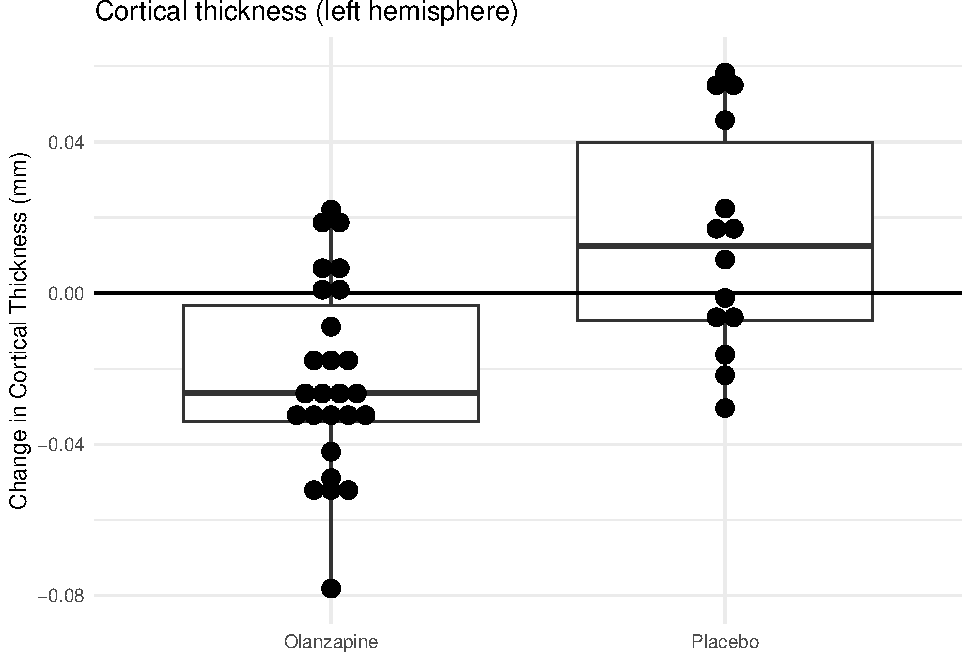
\includegraphics{06_STOPPD_CorticalThickness_byhemi_files/figure-latex/RCT_LCT_boxplot-1.pdf}

\begin{Shaded}
\begin{Highlighting}[]
\CommentTok{#run linear model without covariates}
\NormalTok{  fit_rct <-}\StringTok{ }\KeywordTok{lm}\NormalTok{(LThickness_change }\OperatorTok{~}\StringTok{ }\NormalTok{RandomArm, }\DataTypeTok{data=}\NormalTok{ RCT_CT)}
  \KeywordTok{print}\NormalTok{(fit_rct)}
\end{Highlighting}
\end{Shaded}

\begin{verbatim}
## 
## Call:
## lm(formula = LThickness_change ~ RandomArm, data = RCT_CT)
## 
## Coefficients:
##      (Intercept)  RandomArmPlacebo  
##         -0.02253           0.03659
\end{verbatim}

\begin{Shaded}
\begin{Highlighting}[]
  \KeywordTok{summary}\NormalTok{(fit_rct)}
\end{Highlighting}
\end{Shaded}

\begin{verbatim}
## 
## Call:
## lm(formula = LThickness_change ~ RandomArm, data = RCT_CT)
## 
## Residuals:
##       Min        1Q    Median        3Q       Max 
## -0.055651 -0.018822 -0.003541  0.022344  0.044589 
## 
## Coefficients:
##                   Estimate Std. Error t value Pr(>|t|)    
## (Intercept)      -0.022529   0.005294  -4.255 0.000131 ***
## RandomArmPlacebo  0.036591   0.008949   4.089 0.000217 ***
## ---
## Signif. codes:  0 '***' 0.001 '**' 0.01 '*' 0.05 '.' 0.1 ' ' 1
## 
## Residual standard error: 0.027 on 38 degrees of freedom
## Multiple R-squared:  0.3055, Adjusted R-squared:  0.2873 
## F-statistic: 16.72 on 1 and 38 DF,  p-value: 0.0002168
\end{verbatim}

\begin{Shaded}
\begin{Highlighting}[]
\CommentTok{#run linear model with covariates of sex and age}
\NormalTok{  fit_rct <-}\StringTok{ }\KeywordTok{lm}\NormalTok{(LThickness_change }\OperatorTok{~}\StringTok{ }\NormalTok{RandomArm }\OperatorTok{+}\StringTok{ }\NormalTok{sex }\OperatorTok{+}\StringTok{ }\NormalTok{age, }\DataTypeTok{data=}\NormalTok{ RCT_CT)}
  \KeywordTok{print}\NormalTok{(fit_rct)}
\end{Highlighting}
\end{Shaded}

\begin{verbatim}
## 
## Call:
## lm(formula = LThickness_change ~ RandomArm + sex + age, data = RCT_CT)
## 
## Coefficients:
##      (Intercept)  RandomArmPlacebo              sexM               age  
##       -0.0053535         0.0389342         0.0087658        -0.0004063
\end{verbatim}

\begin{Shaded}
\begin{Highlighting}[]
  \KeywordTok{summary}\NormalTok{(fit_rct)}
\end{Highlighting}
\end{Shaded}

\begin{verbatim}
## 
## Call:
## lm(formula = LThickness_change ~ RandomArm + sex + age, data = RCT_CT)
## 
## Residuals:
##       Min        1Q    Median        3Q       Max 
## -0.054543 -0.019130 -0.001897  0.019599  0.050858 
## 
## Coefficients:
##                    Estimate Std. Error t value Pr(>|t|)    
## (Intercept)      -0.0053535  0.0168885  -0.317 0.753081    
## RandomArmPlacebo  0.0389342  0.0090734   4.291 0.000128 ***
## sexM              0.0087658  0.0087344   1.004 0.322272    
## age              -0.0004063  0.0003132  -1.297 0.202857    
## ---
## Signif. codes:  0 '***' 0.001 '**' 0.01 '*' 0.05 '.' 0.1 ' ' 1
## 
## Residual standard error: 0.02691 on 36 degrees of freedom
## Multiple R-squared:  0.3465, Adjusted R-squared:  0.292 
## F-statistic: 6.363 on 3 and 36 DF,  p-value: 0.001424
\end{verbatim}

\begin{Shaded}
\begin{Highlighting}[]
\CommentTok{#run linear model with covariates of sex and age}
\NormalTok{  fit_rct <-}\StringTok{ }\KeywordTok{lm}\NormalTok{(LThickness_change }\OperatorTok{~}\StringTok{ }\NormalTok{RandomArm }\OperatorTok{+}\StringTok{ }\NormalTok{sex }\OperatorTok{+}\StringTok{ }\NormalTok{age }\OperatorTok{+}\StringTok{ }\NormalTok{site, }\DataTypeTok{data=}\NormalTok{ RCT_CT)}
  \KeywordTok{print}\NormalTok{(fit_rct)}
\end{Highlighting}
\end{Shaded}

\begin{verbatim}
## 
## Call:
## lm(formula = LThickness_change ~ RandomArm + sex + age + site, 
##     data = RCT_CT)
## 
## Coefficients:
##      (Intercept)  RandomArmPlacebo              sexM               age  
##        0.0003982         0.0404923         0.0127657        -0.0003164  
##          siteMAS           siteNKI           sitePMC  
##       -0.0193116        -0.0212567        -0.0287115
\end{verbatim}

\begin{Shaded}
\begin{Highlighting}[]
  \KeywordTok{summary}\NormalTok{(fit_rct)}
\end{Highlighting}
\end{Shaded}

\begin{verbatim}
## 
## Call:
## lm(formula = LThickness_change ~ RandomArm + sex + age + site, 
##     data = RCT_CT)
## 
## Residuals:
##       Min        1Q    Median        3Q       Max 
## -0.045029 -0.013484 -0.001428  0.017054  0.052285 
## 
## Coefficients:
##                    Estimate Std. Error t value Pr(>|t|)    
## (Intercept)       0.0003982  0.0177658   0.022   0.9823    
## RandomArmPlacebo  0.0404923  0.0086868   4.661 4.99e-05 ***
## sexM              0.0127657  0.0083335   1.532   0.1351    
## age              -0.0003164  0.0003244  -0.975   0.3365    
## siteMAS          -0.0193116  0.0110783  -1.743   0.0906 .  
## siteNKI          -0.0212567  0.0105872  -2.008   0.0529 .  
## sitePMC          -0.0287115  0.0130066  -2.207   0.0343 *  
## ---
## Signif. codes:  0 '***' 0.001 '**' 0.01 '*' 0.05 '.' 0.1 ' ' 1
## 
## Residual standard error: 0.02527 on 33 degrees of freedom
## Multiple R-squared:  0.4717, Adjusted R-squared:  0.3757 
## F-statistic: 4.911 on 6 and 33 DF,  p-value: 0.001094
\end{verbatim}

\subsubsection{looking at the same thing for Right
CT}\label{looking-at-the-same-thing-for-right-ct}

\begin{Shaded}
\begin{Highlighting}[]
\CommentTok{#boxplot of difference in thickness (y axis) by randomization group (x axis)}
\KeywordTok{ggplot}\NormalTok{(RCT_CT, }\KeywordTok{aes}\NormalTok{(}\DataTypeTok{x=}\NormalTok{ RandomArm, }\DataTypeTok{y =}\NormalTok{ RThickness_change)) }\OperatorTok{+}\StringTok{ }
\StringTok{     }\KeywordTok{geom_boxplot}\NormalTok{(}\DataTypeTok{outlier.shape =} \OtherTok{NA}\NormalTok{) }\OperatorTok{+}\StringTok{ }
\StringTok{     }\KeywordTok{geom_dotplot}\NormalTok{(}\DataTypeTok{binaxis =} \StringTok{'y'}\NormalTok{, }\DataTypeTok{stackdir =} \StringTok{'center'}\NormalTok{) }\OperatorTok{+}
\StringTok{     }\KeywordTok{geom_hline}\NormalTok{(}\DataTypeTok{yintercept =} \DecValTok{0}\NormalTok{) }\OperatorTok{+}
\StringTok{     }\KeywordTok{ggtitle}\NormalTok{(}\StringTok{"Cortical thickness (right hemisphere)"}\NormalTok{) }\OperatorTok{+}
\StringTok{     }\KeywordTok{xlab}\NormalTok{(}\OtherTok{NULL}\NormalTok{) }\OperatorTok{+}
\StringTok{     }\KeywordTok{ylab}\NormalTok{(}\StringTok{"Change in Cortical Thickness (mm)"}\NormalTok{) }\OperatorTok{+}
\StringTok{     }\KeywordTok{theme_minimal}\NormalTok{()}
\end{Highlighting}
\end{Shaded}

\begin{verbatim}
## `stat_bindot()` using `bins = 30`. Pick better value with `binwidth`.
\end{verbatim}

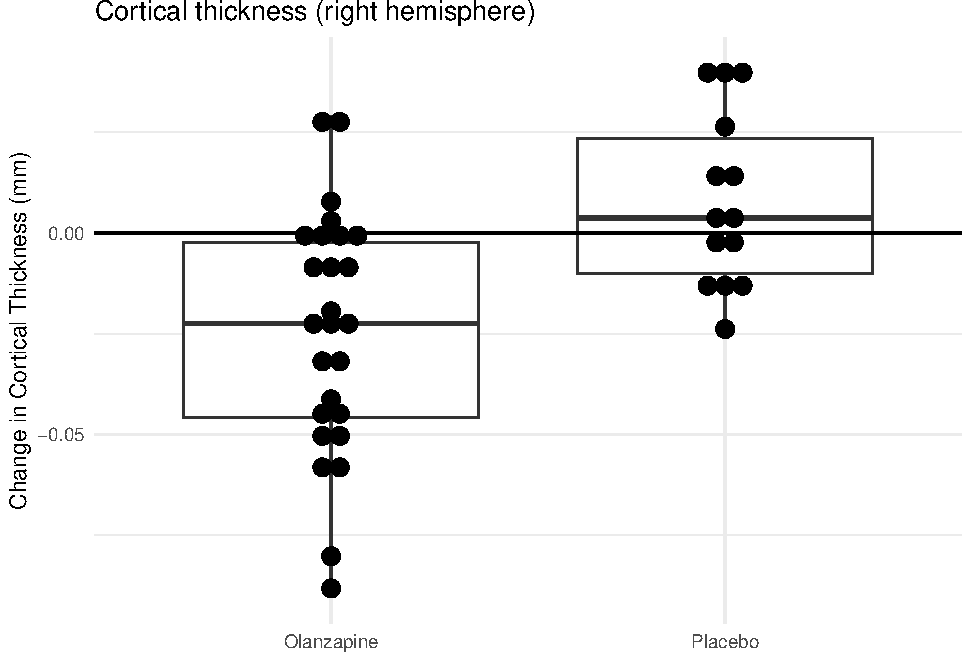
\includegraphics{06_STOPPD_CorticalThickness_byhemi_files/figure-latex/RCT_RCT_boxplot-1.pdf}

\begin{Shaded}
\begin{Highlighting}[]
\CommentTok{#boxplot of difference in thickness (y axis) by randomization group (x axis)}
\NormalTok{RCT_CT }\OperatorTok
\StringTok{  }\KeywordTok{gather}\NormalTok{(TCT, mm, LThickness_change, RThickness_change) }\OperatorTok
\StringTok{  }\KeywordTok{mutate}\NormalTok{(}\DataTypeTok{ThickChange =} \KeywordTok{factor}\NormalTok{(TCT, }\DataTypeTok{levels =} \KeywordTok{c}\NormalTok{(}\StringTok{"LThickness_change"}\NormalTok{, }\StringTok{"RThickness_change"}\NormalTok{),}
                              \DataTypeTok{labels =} \KeywordTok{c}\NormalTok{(}\StringTok{"Left Hemisphere"}\NormalTok{, }\StringTok{"Right Hemisphere"}\NormalTok{))) }\OperatorTok
\KeywordTok{ggplot}\NormalTok{(}\KeywordTok{aes}\NormalTok{(}\DataTypeTok{x=}\NormalTok{ RandomArm, }\DataTypeTok{y =}\NormalTok{ mm)) }\OperatorTok{+}\StringTok{ }
\StringTok{     }\KeywordTok{geom_boxplot}\NormalTok{(}\DataTypeTok{outlier.shape =} \OtherTok{NA}\NormalTok{) }\OperatorTok{+}\StringTok{ }
\StringTok{     }\KeywordTok{geom_dotplot}\NormalTok{(}\DataTypeTok{binaxis =} \StringTok{'y'}\NormalTok{, }\DataTypeTok{stackdir =} \StringTok{'center'}\NormalTok{) }\OperatorTok{+}
\StringTok{     }\KeywordTok{geom_hline}\NormalTok{(}\DataTypeTok{yintercept =} \DecValTok{0}\NormalTok{) }\OperatorTok{+}
\StringTok{     }\KeywordTok{labs}\NormalTok{(}\DataTypeTok{title =} \StringTok{"Change in Cortical Thickness"}\NormalTok{,}\DataTypeTok{x =} \OtherTok{NULL}\NormalTok{, }\DataTypeTok{y =} \StringTok{"Change in Cortical Thickness (mm)"}\NormalTok{) }\OperatorTok{+}
\StringTok{     }\KeywordTok{facet_wrap}\NormalTok{(}\OperatorTok{~}\StringTok{ }\NormalTok{ThickChange) }\OperatorTok{+}
\StringTok{     }\KeywordTok{theme_bw}\NormalTok{()}
\end{Highlighting}
\end{Shaded}

\begin{verbatim}
## `stat_bindot()` using `bins = 30`. Pick better value with `binwidth`.
\end{verbatim}

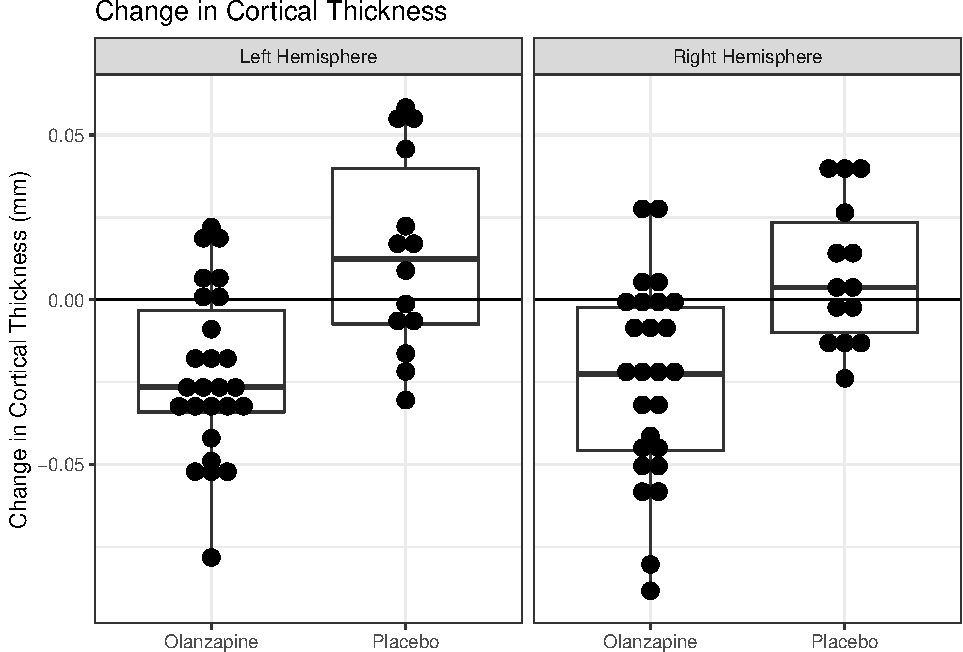
\includegraphics{06_STOPPD_CorticalThickness_byhemi_files/figure-latex/RCT_CT_facet_boxplot-1.pdf}

\begin{Shaded}
\begin{Highlighting}[]
\CommentTok{#run linear model without covariates}
\NormalTok{  fit_rct <-}\StringTok{ }\KeywordTok{lm}\NormalTok{(RThickness_change }\OperatorTok{~}\StringTok{ }\NormalTok{RandomArm, }\DataTypeTok{data=}\NormalTok{ RCT_CT)}
  \KeywordTok{print}\NormalTok{(fit_rct)}
\end{Highlighting}
\end{Shaded}

\begin{verbatim}
## 
## Call:
## lm(formula = RThickness_change ~ RandomArm, data = RCT_CT)
## 
## Coefficients:
##      (Intercept)  RandomArmPlacebo  
##         -0.02434           0.03260
\end{verbatim}

\begin{Shaded}
\begin{Highlighting}[]
  \KeywordTok{summary}\NormalTok{(fit_rct)}
\end{Highlighting}
\end{Shaded}

\begin{verbatim}
## 
## Call:
## lm(formula = RThickness_change ~ RandomArm, data = RCT_CT)
## 
## Residuals:
##      Min       1Q   Median       3Q      Max 
## -0.06395 -0.02029  0.00013  0.02178  0.05351 
## 
## Coefficients:
##                   Estimate Std. Error t value Pr(>|t|)    
## (Intercept)      -0.024340   0.005360  -4.542  5.5e-05 ***
## RandomArmPlacebo  0.032596   0.009059   3.598 0.000912 ***
## ---
## Signif. codes:  0 '***' 0.001 '**' 0.01 '*' 0.05 '.' 0.1 ' ' 1
## 
## Residual standard error: 0.02733 on 38 degrees of freedom
## Multiple R-squared:  0.2541, Adjusted R-squared:  0.2345 
## F-statistic: 12.95 on 1 and 38 DF,  p-value: 0.0009116
\end{verbatim}

\begin{Shaded}
\begin{Highlighting}[]
\CommentTok{#run linear model with covariates of sex and age}
\NormalTok{  fit_rct <-}\StringTok{ }\KeywordTok{lm}\NormalTok{(RThickness_change }\OperatorTok{~}\StringTok{ }\NormalTok{RandomArm }\OperatorTok{+}\StringTok{ }\NormalTok{sex }\OperatorTok{+}\StringTok{ }\NormalTok{age, }\DataTypeTok{data=}\NormalTok{ RCT_CT)}
  \KeywordTok{print}\NormalTok{(fit_rct)}
\end{Highlighting}
\end{Shaded}

\begin{verbatim}
## 
## Call:
## lm(formula = RThickness_change ~ RandomArm + sex + age, data = RCT_CT)
## 
## Coefficients:
##      (Intercept)  RandomArmPlacebo              sexM               age  
##       -0.0097657         0.0336641        -0.0044117        -0.0002401
\end{verbatim}

\begin{Shaded}
\begin{Highlighting}[]
  \KeywordTok{summary}\NormalTok{(fit_rct)}
\end{Highlighting}
\end{Shaded}

\begin{verbatim}
## 
## Call:
## lm(formula = RThickness_change ~ RandomArm + sex + age, data = RCT_CT)
## 
## Residuals:
##      Min       1Q   Median       3Q      Max 
## -0.06700 -0.01799 -0.00128  0.01847  0.04950 
## 
## Coefficients:
##                    Estimate Std. Error t value Pr(>|t|)    
## (Intercept)      -0.0097657  0.0173882  -0.562 0.577851    
## RandomArmPlacebo  0.0336641  0.0093419   3.604 0.000941 ***
## sexM             -0.0044117  0.0089928  -0.491 0.626698    
## age              -0.0002401  0.0003225  -0.744 0.461500    
## ---
## Signif. codes:  0 '***' 0.001 '**' 0.01 '*' 0.05 '.' 0.1 ' ' 1
## 
## Residual standard error: 0.0277 on 36 degrees of freedom
## Multiple R-squared:  0.2739, Adjusted R-squared:  0.2134 
## F-statistic: 4.527 on 3 and 36 DF,  p-value: 0.008575
\end{verbatim}

\begin{Shaded}
\begin{Highlighting}[]
\CommentTok{#run linear model with covariates of sex and age}
\NormalTok{  fit_rct <-}\StringTok{ }\KeywordTok{lm}\NormalTok{(RThickness_change }\OperatorTok{~}\StringTok{ }\NormalTok{RandomArm }\OperatorTok{+}\StringTok{ }\NormalTok{sex }\OperatorTok{+}\StringTok{ }\NormalTok{age }\OperatorTok{+}\StringTok{ }\NormalTok{site, }\DataTypeTok{data=}\NormalTok{ RCT_CT)}
  \KeywordTok{print}\NormalTok{(fit_rct)}
\end{Highlighting}
\end{Shaded}

\begin{verbatim}
## 
## Call:
## lm(formula = RThickness_change ~ RandomArm + sex + age + site, 
##     data = RCT_CT)
## 
## Coefficients:
##      (Intercept)  RandomArmPlacebo              sexM               age  
##       -1.111e-02         3.389e-02        -1.632e-03        -9.043e-05  
##          siteMAS           siteNKI           sitePMC  
##       -1.010e-02        -1.044e-02        -2.463e-02
\end{verbatim}

\begin{Shaded}
\begin{Highlighting}[]
  \KeywordTok{summary}\NormalTok{(fit_rct)}
\end{Highlighting}
\end{Shaded}

\begin{verbatim}
## 
## Call:
## lm(formula = RThickness_change ~ RandomArm + sex + age + site, 
##     data = RCT_CT)
## 
## Residuals:
##       Min        1Q    Median        3Q       Max 
## -0.072836 -0.015554  0.000948  0.019346  0.044262 
## 
## Coefficients:
##                    Estimate Std. Error t value Pr(>|t|)   
## (Intercept)      -1.111e-02  1.939e-02  -0.573  0.57042   
## RandomArmPlacebo  3.389e-02  9.480e-03   3.575  0.00111 **
## sexM             -1.632e-03  9.095e-03  -0.179  0.85869   
## age              -9.043e-05  3.540e-04  -0.255  0.79998   
## siteMAS          -1.010e-02  1.209e-02  -0.835  0.40968   
## siteNKI          -1.044e-02  1.155e-02  -0.903  0.37287   
## sitePMC          -2.463e-02  1.419e-02  -1.735  0.09208 . 
## ---
## Signif. codes:  0 '***' 0.001 '**' 0.01 '*' 0.05 '.' 0.1 ' ' 1
## 
## Residual standard error: 0.02758 on 33 degrees of freedom
## Multiple R-squared:  0.3405, Adjusted R-squared:  0.2206 
## F-statistic:  2.84 on 6 and 33 DF,  p-value: 0.02429
\end{verbatim}

\subsection{RCT \& Relapse (with time as
factor)}\label{rct-relapse-with-time-as-factor}

\begin{Shaded}
\begin{Highlighting}[]
\CommentTok{#restructure data for RCT & Relapse participants (N=72)}
\NormalTok{  RCTRelapse_LCT <-}\StringTok{ }\NormalTok{df }\OperatorTok
\StringTok{    }\KeywordTok{gather}\NormalTok{(thick_oldcolname, thickness, LThickness_}\DecValTok{01}\NormalTok{, LThickness_}\DecValTok{02}\NormalTok{) }\OperatorTok
\StringTok{    }\KeywordTok{mutate}\NormalTok{(}\DataTypeTok{model_days =} \KeywordTok{if_else}\NormalTok{(thick_oldcolname }\OperatorTok{==}\StringTok{ "LThickness_01"}\NormalTok{, }\DecValTok{1}\NormalTok{, dateDiff))}

\NormalTok{RCTRelapse_LCT }\OperatorTok\StringTok{ }\KeywordTok{filter}\NormalTok{(model_days }\OperatorTok{==}\StringTok{ }\DecValTok{1}\NormalTok{) }\OperatorTok\StringTok{ }\KeywordTok{count}\NormalTok{(randomization) }\OperatorTok\StringTok{ }\NormalTok{knitr}\OperatorTok{::}\KeywordTok{kable}\NormalTok{() }
\end{Highlighting}
\end{Shaded}

\begin{tabular}{l|r}
\hline
randomization & n\\
\hline
O & 38\\
\hline
P & 34\\
\hline
\end{tabular}

\begin{Shaded}
\begin{Highlighting}[]
\CommentTok{#plot all data, including outlier (participant 210030)}
\NormalTok{  RCTRelapse_LCT }\OperatorTok
\StringTok{   }\KeywordTok{ggplot}\NormalTok{(}\KeywordTok{aes}\NormalTok{(}\DataTypeTok{x=}\NormalTok{model_days, }\DataTypeTok{y=}\NormalTok{thickness, }\DataTypeTok{colour=}\NormalTok{RandomArm)) }\OperatorTok{+}\StringTok{ }
\StringTok{   }\KeywordTok{geom_point}\NormalTok{() }\OperatorTok{+}\StringTok{ }
\StringTok{   }\KeywordTok{geom_line}\NormalTok{(}\KeywordTok{aes}\NormalTok{(}\DataTypeTok{group=}\NormalTok{STUDYID), }\DataTypeTok{alpha =} \FloatTok{0.5}\NormalTok{) }\OperatorTok{+}\StringTok{ }
\StringTok{   }\KeywordTok{geom_smooth}\NormalTok{(}\DataTypeTok{method=}\StringTok{"lm"}\NormalTok{, }\DataTypeTok{formula=}\NormalTok{y}\OperatorTok{~}\KeywordTok{poly}\NormalTok{(x,}\DecValTok{1}\NormalTok{)) }\OperatorTok{+}
\StringTok{   }\KeywordTok{ggtitle}\NormalTok{(}\StringTok{"Cortical thickness in left hemisphere over time"}\NormalTok{) }\OperatorTok{+}
\StringTok{   }\KeywordTok{labs}\NormalTok{(}\DataTypeTok{x =} \StringTok{"Days between MRIs"}\NormalTok{, }\DataTypeTok{y =} \StringTok{"Cortical Thickness (mm)"}\NormalTok{, }\DataTypeTok{colour =} \OtherTok{NULL}\NormalTok{) }\OperatorTok{+}
\StringTok{   }\KeywordTok{theme_minimal}\NormalTok{()}
\end{Highlighting}
\end{Shaded}

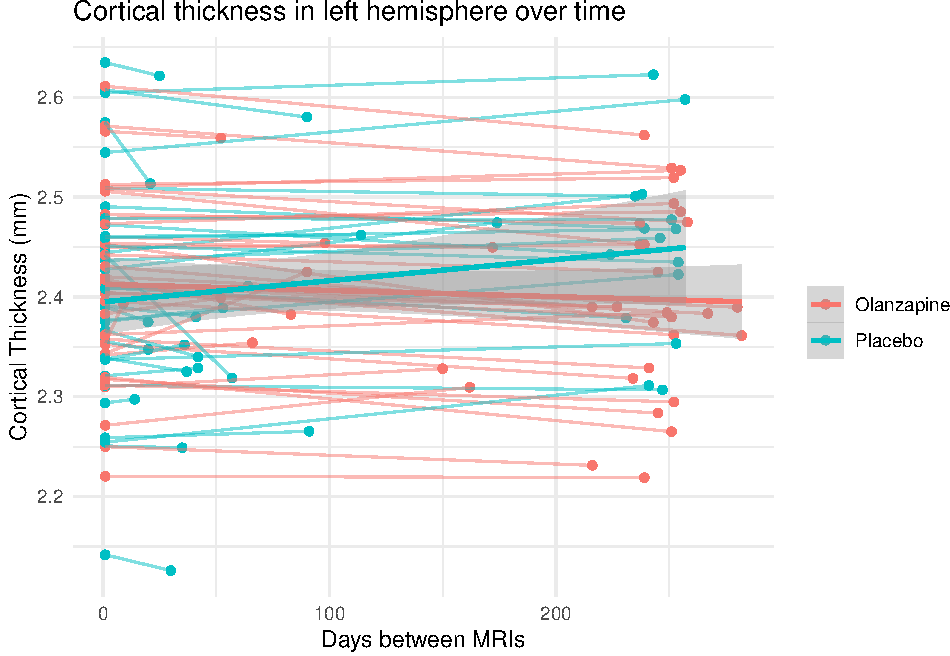
\includegraphics{06_STOPPD_CorticalThickness_byhemi_files/figure-latex/RCTRelapse_LCT_plot-1.pdf}

\begin{Shaded}
\begin{Highlighting}[]
\CommentTok{#run mixed linear model, with covariates}
\NormalTok{  fit_all <-}\StringTok{ }\KeywordTok{lmer}\NormalTok{(thickness }\OperatorTok{~}\StringTok{ }\NormalTok{RandomArm}\OperatorTok{*}\NormalTok{model_days }\OperatorTok{+}\StringTok{ }\NormalTok{sex }\OperatorTok{+}\StringTok{ }\NormalTok{age }\OperatorTok{+}\StringTok{ }\NormalTok{(}\DecValTok{1}\OperatorTok{|}\NormalTok{STUDYID), }\DataTypeTok{data=}\NormalTok{ RCTRelapse_LCT)}
  \KeywordTok{summary}\NormalTok{(fit_all)}
\end{Highlighting}
\end{Shaded}

\begin{verbatim}
## Linear mixed model fit by REML. t-tests use Satterthwaite's method [
## lmerModLmerTest]
## Formula: thickness ~ RandomArm * model_days + sex + age + (1 | STUDYID)
##    Data: RCTRelapse_LCT
## 
## REML criterion at convergence: -396
## 
## Scaled residuals: 
##      Min       1Q   Median       3Q      Max 
## -2.89073 -0.39603 -0.02082  0.40944  2.76834 
## 
## Random effects:
##  Groups   Name        Variance  Std.Dev.
##  STUDYID  (Intercept) 0.0054535 0.07385 
##  Residual             0.0004953 0.02225 
## Number of obs: 144, groups:  STUDYID, 72
## 
## Fixed effects:
##                               Estimate Std. Error         df t value
## (Intercept)                  2.639e+00  3.484e-02  6.864e+01  75.756
## RandomArmPlacebo            -2.035e-03  1.816e-02  7.233e+01  -0.112
## model_days                  -8.012e-05  2.340e-05  7.056e+01  -3.424
## sexM                        -6.099e-03  1.792e-02  6.784e+01  -0.340
## age                         -4.053e-03  5.853e-04  6.785e+01  -6.924
## RandomArmPlacebo:model_days  1.297e-04  3.942e-05  7.148e+01   3.291
##                             Pr(>|t|)    
## (Intercept)                  < 2e-16 ***
## RandomArmPlacebo             0.91106    
## model_days                   0.00103 ** 
## sexM                         0.73470    
## age                         1.96e-09 ***
## RandomArmPlacebo:model_days  0.00155 ** 
## ---
## Signif. codes:  0 '***' 0.001 '**' 0.01 '*' 0.05 '.' 0.1 ' ' 1
## 
## Correlation of Fixed Effects:
##             (Intr) RndmAP mdl_dy sexM   age   
## RndmArmPlcb -0.206                            
## model_days  -0.077  0.133                     
## sexM        -0.171  0.036  0.001              
## age         -0.901 -0.053  0.008 -0.079       
## RndmArmPl:_  0.043 -0.176 -0.594  0.004 -0.003
\end{verbatim}

\begin{Shaded}
\begin{Highlighting}[]
\CommentTok{#run mixed linear model, with covariates}
\NormalTok{  fit_all <-}\StringTok{ }\KeywordTok{lmer}\NormalTok{(thickness }\OperatorTok{~}\StringTok{ }\NormalTok{RandomArm}\OperatorTok{*}\NormalTok{model_days }\OperatorTok{+}\StringTok{ }\NormalTok{sex }\OperatorTok{+}\StringTok{ }\NormalTok{age }\OperatorTok{+}\StringTok{ }\NormalTok{site }\OperatorTok{+}\StringTok{ }\NormalTok{(}\DecValTok{1}\OperatorTok{|}\NormalTok{STUDYID), }\DataTypeTok{data=}\NormalTok{ RCTRelapse_LCT)}
  \KeywordTok{summary}\NormalTok{(fit_all)}
\end{Highlighting}
\end{Shaded}

\begin{verbatim}
## Linear mixed model fit by REML. t-tests use Satterthwaite's method [
## lmerModLmerTest]
## Formula: thickness ~ RandomArm * model_days + sex + age + site + (1 |  
##     STUDYID)
##    Data: RCTRelapse_LCT
## 
## REML criterion at convergence: -380.4
## 
## Scaled residuals: 
##      Min       1Q   Median       3Q      Max 
## -2.93368 -0.37860 -0.00129  0.40530  2.72488 
## 
## Random effects:
##  Groups   Name        Variance  Std.Dev.
##  STUDYID  (Intercept) 0.0055987 0.07482 
##  Residual             0.0004952 0.02225 
## Number of obs: 144, groups:  STUDYID, 72
## 
## Fixed effects:
##                               Estimate Std. Error         df t value
## (Intercept)                  2.640e+00  3.703e-02  6.556e+01  71.309
## RandomArmPlacebo            -1.963e-03  1.863e-02  6.894e+01  -0.105
## model_days                  -8.021e-05  2.341e-05  7.051e+01  -3.427
## sexM                        -8.192e-03  1.840e-02  6.485e+01  -0.445
## age                         -4.101e-03  5.970e-04  6.486e+01  -6.869
## siteMAS                     -6.325e-03  2.335e-02  6.486e+01  -0.271
## siteNKI                      1.359e-04  2.587e-02  6.486e+01   0.005
## sitePMC                      2.516e-02  2.662e-02  6.485e+01   0.945
## RandomArmPlacebo:model_days  1.296e-04  3.942e-05  7.143e+01   3.286
##                             Pr(>|t|)    
## (Intercept)                  < 2e-16 ***
## RandomArmPlacebo             0.91640    
## model_days                   0.00102 ** 
## sexM                         0.65759    
## age                         2.98e-09 ***
## siteMAS                      0.78731    
## siteNKI                      0.99582    
## sitePMC                      0.34814    
## RandomArmPlacebo:model_days  0.00158 ** 
## ---
## Signif. codes:  0 '***' 0.001 '**' 0.01 '*' 0.05 '.' 0.1 ' ' 1
## 
## Correlation of Fixed Effects:
##             (Intr) RndmAP mdl_dy sexM   age    sitMAS sitNKI sitPMC
## RndmArmPlcb -0.145                                                 
## model_days  -0.074  0.129                                          
## sexM        -0.130  0.054  0.002                                   
## age         -0.880 -0.064  0.009 -0.076                            
## siteMAS     -0.291 -0.145  0.009 -0.066  0.108                     
## siteNKI     -0.174 -0.119 -0.010 -0.119  0.010  0.357              
## sitePMC     -0.153 -0.088  0.000 -0.144 -0.009  0.343  0.319       
## RndmArmPl:_  0.040 -0.172 -0.594  0.003 -0.003  0.000  0.009  0.002
\end{verbatim}

\subsubsection{Running the right hemisphere
RCTRelapse}\label{running-the-right-hemisphere-rctrelapse}

\begin{Shaded}
\begin{Highlighting}[]
\CommentTok{#restructure data for RCT & Relapse participants (N=72)}
\NormalTok{  RCTRelapse_RCT <-}\StringTok{ }\NormalTok{df }\OperatorTok
\StringTok{    }\KeywordTok{gather}\NormalTok{(thick_oldcolname, thickness, RThickness_}\DecValTok{01}\NormalTok{, RThickness_}\DecValTok{02}\NormalTok{) }\OperatorTok
\StringTok{    }\KeywordTok{mutate}\NormalTok{(}\DataTypeTok{model_days =} \KeywordTok{if_else}\NormalTok{(thick_oldcolname }\OperatorTok{==}\StringTok{ "RThickness_01"}\NormalTok{, }\DecValTok{1}\NormalTok{, dateDiff))}

\CommentTok{#plot all data, including outlier (participant 210030)}
\NormalTok{  RCTRelapse_RCT }\OperatorTok
\StringTok{   }\KeywordTok{ggplot}\NormalTok{(}\KeywordTok{aes}\NormalTok{(}\DataTypeTok{x=}\NormalTok{model_days, }\DataTypeTok{y=}\NormalTok{thickness, }\DataTypeTok{colour=}\NormalTok{RandomArm)) }\OperatorTok{+}\StringTok{ }
\StringTok{   }\KeywordTok{geom_point}\NormalTok{() }\OperatorTok{+}\StringTok{ }
\StringTok{   }\KeywordTok{geom_line}\NormalTok{(}\KeywordTok{aes}\NormalTok{(}\DataTypeTok{group=}\NormalTok{STUDYID), }\DataTypeTok{alpha =} \FloatTok{0.5}\NormalTok{) }\OperatorTok{+}\StringTok{ }
\StringTok{   }\KeywordTok{geom_smooth}\NormalTok{(}\DataTypeTok{method=}\StringTok{"lm"}\NormalTok{, }\DataTypeTok{formula=}\NormalTok{y}\OperatorTok{~}\KeywordTok{poly}\NormalTok{(x,}\DecValTok{1}\NormalTok{)) }\OperatorTok{+}
\StringTok{   }\KeywordTok{ggtitle}\NormalTok{(}\StringTok{"Cortical thickness in right hemisphere over time"}\NormalTok{) }\OperatorTok{+}
\StringTok{   }\KeywordTok{labs}\NormalTok{(}\DataTypeTok{x =} \StringTok{"Days between MRIs"}\NormalTok{, }\DataTypeTok{y =} \StringTok{"Cortical Thickness (mm)"}\NormalTok{, }\DataTypeTok{colour =} \OtherTok{NULL}\NormalTok{) }\OperatorTok{+}
\StringTok{   }\KeywordTok{theme_minimal}\NormalTok{()}
\end{Highlighting}
\end{Shaded}

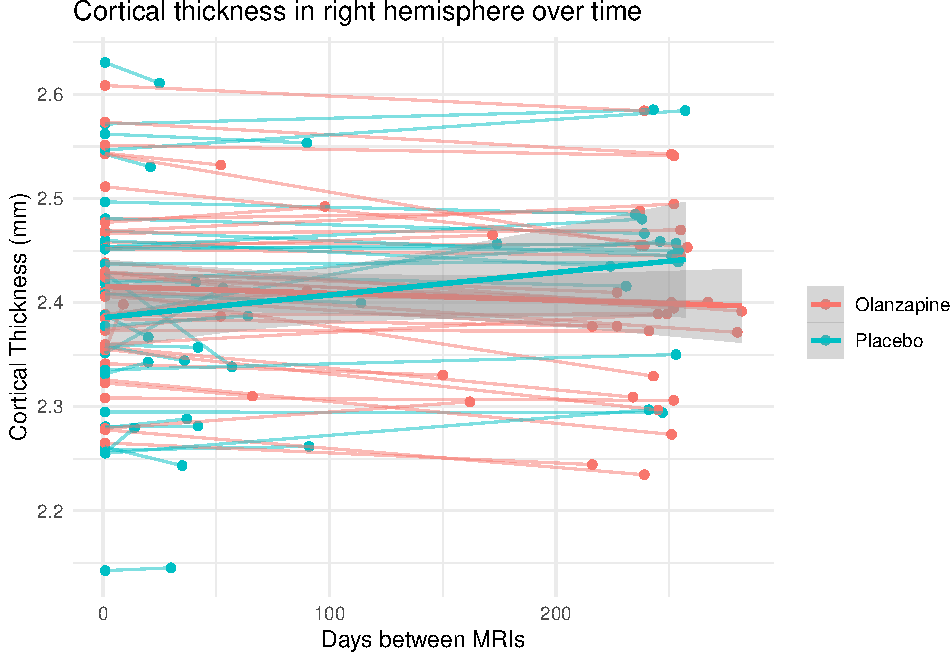
\includegraphics{06_STOPPD_CorticalThickness_byhemi_files/figure-latex/RCTRelapse_RCT_plot-1.pdf}

\begin{Shaded}
\begin{Highlighting}[]
\CommentTok{#run mixed linear model, with covariates}
\NormalTok{  fit_all <-}\StringTok{ }\KeywordTok{lmer}\NormalTok{(thickness }\OperatorTok{~}\StringTok{ }\NormalTok{RandomArm}\OperatorTok{*}\NormalTok{model_days }\OperatorTok{+}\StringTok{ }\NormalTok{sex }\OperatorTok{+}\StringTok{ }\NormalTok{age }\OperatorTok{+}\StringTok{ }\NormalTok{(}\DecValTok{1}\OperatorTok{|}\NormalTok{STUDYID), }\DataTypeTok{data=}\NormalTok{ RCTRelapse_RCT)}
  \KeywordTok{summary}\NormalTok{(fit_all)}
\end{Highlighting}
\end{Shaded}

\begin{verbatim}
## Linear mixed model fit by REML. t-tests use Satterthwaite's method [
## lmerModLmerTest]
## Formula: thickness ~ RandomArm * model_days + sex + age + (1 | STUDYID)
##    Data: RCTRelapse_RCT
## 
## REML criterion at convergence: -409
## 
## Scaled residuals: 
##      Min       1Q   Median       3Q      Max 
## -2.34720 -0.42608 -0.01215  0.43733  2.27881 
## 
## Random effects:
##  Groups   Name        Variance  Std.Dev.
##  STUDYID  (Intercept) 0.0057442 0.07579 
##  Residual             0.0003947 0.01987 
## Number of obs: 144, groups:  STUDYID, 72
## 
## Fixed effects:
##                               Estimate Std. Error         df t value
## (Intercept)                  2.618e+00  3.554e-02  6.847e+01  73.658
## RandomArmPlacebo            -1.455e-02  1.847e-02  7.131e+01  -0.788
## model_days                  -8.813e-05  2.090e-05  7.041e+01  -4.216
## sexM                        -7.789e-03  1.830e-02  6.786e+01  -0.426
## age                         -3.588e-03  5.975e-04  6.786e+01  -6.004
## RandomArmPlacebo:model_days  1.281e-04  3.524e-05  7.112e+01   3.635
##                             Pr(>|t|)    
## (Intercept)                  < 2e-16 ***
## RandomArmPlacebo            0.433361    
## model_days                  7.28e-05 ***
## sexM                        0.671706    
## age                         8.40e-08 ***
## RandomArmPlacebo:model_days 0.000522 ***
## ---
## Signif. codes:  0 '***' 0.001 '**' 0.01 '*' 0.05 '.' 0.1 ' ' 1
## 
## Correlation of Fixed Effects:
##             (Intr) RndmAP mdl_dy sexM   age   
## RndmArmPlcb -0.205                            
## model_days  -0.067  0.117                     
## sexM        -0.172  0.036  0.001              
## age         -0.902 -0.053  0.007 -0.079       
## RndmArmPl:_  0.037 -0.155 -0.593  0.003 -0.002
\end{verbatim}

\begin{Shaded}
\begin{Highlighting}[]
\CommentTok{#run mixed linear model, with covariates}
\NormalTok{  fit_all <-}\StringTok{ }\KeywordTok{lmer}\NormalTok{(thickness }\OperatorTok{~}\StringTok{ }\NormalTok{RandomArm}\OperatorTok{*}\NormalTok{model_days }\OperatorTok{+}\StringTok{ }\NormalTok{sex }\OperatorTok{+}\StringTok{ }\NormalTok{age }\OperatorTok{+}\StringTok{ }\NormalTok{site }\OperatorTok{+}\StringTok{ }\NormalTok{(}\DecValTok{1}\OperatorTok{|}\NormalTok{STUDYID), }\DataTypeTok{data=}\NormalTok{ RCTRelapse_RCT)}
  \KeywordTok{summary}\NormalTok{(fit_all)}
\end{Highlighting}
\end{Shaded}

\begin{verbatim}
## Linear mixed model fit by REML. t-tests use Satterthwaite's method [
## lmerModLmerTest]
## Formula: thickness ~ RandomArm * model_days + sex + age + site + (1 |  
##     STUDYID)
##    Data: RCTRelapse_RCT
## 
## REML criterion at convergence: -393.2
## 
## Scaled residuals: 
##      Min       1Q   Median       3Q      Max 
## -2.37660 -0.44552 -0.00537  0.43115  2.24882 
## 
## Random effects:
##  Groups   Name        Variance  Std.Dev.
##  STUDYID  (Intercept) 0.0059298 0.07701 
##  Residual             0.0003947 0.01987 
## Number of obs: 144, groups:  STUDYID, 72
## 
## Fixed effects:
##                               Estimate Std. Error         df t value
## (Intercept)                  2.619e+00  3.788e-02  6.541e+01  69.150
## RandomArmPlacebo            -1.446e-02  1.900e-02  6.800e+01  -0.761
## model_days                  -8.825e-05  2.091e-05  7.037e+01  -4.221
## sexM                        -9.731e-03  1.883e-02  6.487e+01  -0.517
## age                         -3.638e-03  6.112e-04  6.487e+01  -5.952
## siteMAS                     -7.805e-03  2.390e-02  6.488e+01  -0.327
## siteNKI                      4.352e-03  2.649e-02  6.488e+01   0.164
## sitePMC                      2.024e-02  2.725e-02  6.487e+01   0.743
## RandomArmPlacebo:model_days  1.280e-04  3.524e-05  7.108e+01   3.631
##                             Pr(>|t|)    
## (Intercept)                  < 2e-16 ***
## RandomArmPlacebo            0.449288    
## model_days                  7.14e-05 ***
## sexM                        0.607158    
## age                         1.18e-07 ***
## siteMAS                     0.745036    
## siteNKI                     0.870002    
## sitePMC                     0.460300    
## RandomArmPlacebo:model_days 0.000529 ***
## ---
## Signif. codes:  0 '***' 0.001 '**' 0.01 '*' 0.05 '.' 0.1 ' ' 1
## 
## Correlation of Fixed Effects:
##             (Intr) RndmAP mdl_dy sexM   age    sitMAS sitNKI sitPMC
## RndmArmPlcb -0.144                                                 
## model_days  -0.064  0.113                                          
## sexM        -0.130  0.055  0.002                                   
## age         -0.881 -0.065  0.008 -0.076                            
## siteMAS     -0.291 -0.146  0.007 -0.066  0.108                     
## siteNKI     -0.175 -0.119 -0.008 -0.119  0.010  0.357              
## sitePMC     -0.153 -0.089  0.000 -0.144 -0.009  0.343  0.319       
## RndmArmPl:_  0.035 -0.151 -0.593  0.003 -0.003  0.000  0.008  0.002
\end{verbatim}

\section{Surface Area Analysis}\label{surface-area-analysis}

This script analyses hemisphere wide surface area

\begin{Shaded}
\begin{Highlighting}[]
\CommentTok{#load libraries}
\KeywordTok{library}\NormalTok{(tidyverse)}
\KeywordTok{library}\NormalTok{(lme4)}
\KeywordTok{library}\NormalTok{(lmerTest)}
\KeywordTok{library}\NormalTok{(growthmodels)}


\CommentTok{#bring in data }
\NormalTok{df <-}\StringTok{ }\KeywordTok{read_csv}\NormalTok{(}\StringTok{'../generated_csvs/STOPPD_participantsCT_20181111.csv'}\NormalTok{) }\CommentTok{#generated by 05_STOPPD_error in prepartion of Jason Lerch meeting}
\end{Highlighting}
\end{Shaded}

\begin{Shaded}
\begin{Highlighting}[]
\CommentTok{#make sure that STUDYID is an interger not a number}
\NormalTok{  df}\OperatorTok{$}\NormalTok{STUDYID <-}\StringTok{ }\KeywordTok{as.character}\NormalTok{(df}\OperatorTok{$}\NormalTok{STUDYID)}

\CommentTok{#make sure that dateDiff is a number, not an interger}
\NormalTok{  df}\OperatorTok{$}\NormalTok{dateDiff <-}\StringTok{ }\KeywordTok{as.numeric}\NormalTok{(df}\OperatorTok{$}\NormalTok{dateDiff)}

\CommentTok{# label the randomization variable  }
\NormalTok{df}\OperatorTok{$}\NormalTok{RandomArm <-}\StringTok{ }\KeywordTok{factor}\NormalTok{(df}\OperatorTok{$}\NormalTok{randomization, }
                       \DataTypeTok{levels =} \KeywordTok{c}\NormalTok{(}\StringTok{"O"}\NormalTok{, }\StringTok{"P"}\NormalTok{),}
                       \DataTypeTok{labels =} \KeywordTok{c}\NormalTok{(}\StringTok{"Olanzapine"}\NormalTok{, }\StringTok{"Placebo"}\NormalTok{))}

\CommentTok{#restructure data for RCT completers' only (N=40)}
\NormalTok{  RCT_SA <-}\StringTok{ }\NormalTok{df }\OperatorTok
\StringTok{    }\KeywordTok{filter}\NormalTok{(category }\OperatorTok{==}\StringTok{ "RCT"}\NormalTok{) }

\CommentTok{#write out clean dataframe}
 \CommentTok{# write.csv(RCT_CT, '../generated_data/df_leftCT.csv', row.names=FALSE)}
\end{Highlighting}
\end{Shaded}

\subsection{RCT only}\label{rct-only-1}

\begin{Shaded}
\begin{Highlighting}[]
\NormalTok{RCT_SA }\OperatorTok\StringTok{ }\KeywordTok{count}\NormalTok{(randomization) }\OperatorTok\StringTok{ }\NormalTok{knitr}\OperatorTok{::}\KeywordTok{kable}\NormalTok{() }
\end{Highlighting}
\end{Shaded}

\begin{tabular}{l|r}
\hline
randomization & n\\
\hline
O & 26\\
\hline
P & 14\\
\hline
\end{tabular}

\begin{Shaded}
\begin{Highlighting}[]
\CommentTok{#boxplot of difference in thickness (y axis) by randomization group (x axis)}
\KeywordTok{ggplot}\NormalTok{(RCT_SA, }\KeywordTok{aes}\NormalTok{(}\DataTypeTok{x=}\NormalTok{ RandomArm, }\DataTypeTok{y =}\NormalTok{ LSurfArea_change)) }\OperatorTok{+}\StringTok{ }
\StringTok{     }\KeywordTok{geom_boxplot}\NormalTok{(}\DataTypeTok{outlier.shape =} \OtherTok{NA}\NormalTok{) }\OperatorTok{+}\StringTok{ }
\StringTok{     }\KeywordTok{geom_dotplot}\NormalTok{(}\DataTypeTok{binaxis =} \StringTok{'y'}\NormalTok{, }\DataTypeTok{stackdir =} \StringTok{'center'}\NormalTok{) }\OperatorTok{+}
\StringTok{     }\KeywordTok{geom_hline}\NormalTok{(}\DataTypeTok{yintercept =} \DecValTok{0}\NormalTok{) }\OperatorTok{+}
\StringTok{     }\KeywordTok{ggtitle}\NormalTok{(}\StringTok{"Surface Area (left hemisphere)"}\NormalTok{) }\OperatorTok{+}
\StringTok{     }\KeywordTok{xlab}\NormalTok{(}\OtherTok{NULL}\NormalTok{) }\OperatorTok{+}
\StringTok{     }\KeywordTok{ylab}\NormalTok{(}\StringTok{"Change in Surface Area"}\NormalTok{) }\OperatorTok{+}
\StringTok{     }\KeywordTok{theme_minimal}\NormalTok{()}
\end{Highlighting}
\end{Shaded}

\begin{verbatim}
## `stat_bindot()` using `bins = 30`. Pick better value with `binwidth`.
\end{verbatim}

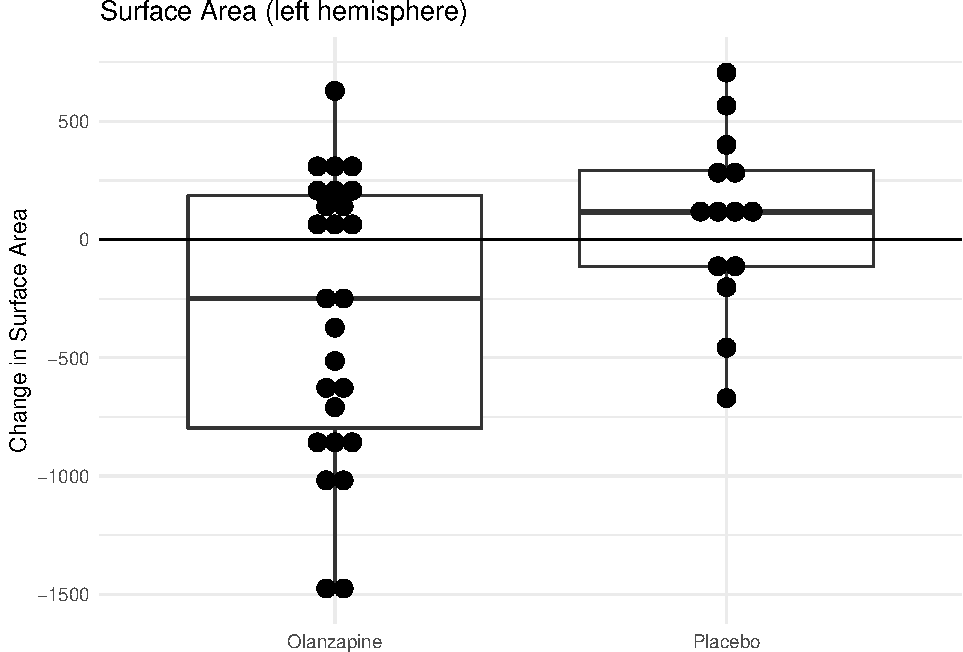
\includegraphics{07_STOPPD_CorticalSurfaceArea_byhemi_files/figure-latex/RCT_LSA_boxplot-1.pdf}

\begin{Shaded}
\begin{Highlighting}[]
\CommentTok{#run linear model without covariates}
\NormalTok{  fit_rct <-}\StringTok{ }\KeywordTok{lm}\NormalTok{(LSurfArea_change }\OperatorTok{~}\StringTok{ }\NormalTok{RandomArm, }\DataTypeTok{data=}\NormalTok{ RCT_SA)}
  \KeywordTok{print}\NormalTok{(fit_rct)}
\end{Highlighting}
\end{Shaded}

\begin{verbatim}
## 
## Call:
## lm(formula = LSurfArea_change ~ RandomArm, data = RCT_SA)
## 
## Coefficients:
##      (Intercept)  RandomArmPlacebo  
##           -316.6             399.2
\end{verbatim}

\begin{Shaded}
\begin{Highlighting}[]
  \KeywordTok{summary}\NormalTok{(fit_rct)}
\end{Highlighting}
\end{Shaded}

\begin{verbatim}
## 
## Call:
## lm(formula = LSurfArea_change ~ RandomArm, data = RCT_SA)
## 
## Residuals:
##     Min      1Q  Median      3Q     Max 
## -1182.2  -333.1    43.8   441.8   945.5 
## 
## Coefficients:
##                  Estimate Std. Error t value Pr(>|t|)   
## (Intercept)        -316.6      103.1   -3.07  0.00394 **
## RandomArmPlacebo    399.2      174.3    2.29  0.02763 * 
## ---
## Signif. codes:  0 '***' 0.001 '**' 0.01 '*' 0.05 '.' 0.1 ' ' 1
## 
## Residual standard error: 525.8 on 38 degrees of freedom
## Multiple R-squared:  0.1213, Adjusted R-squared:  0.09819 
## F-statistic: 5.246 on 1 and 38 DF,  p-value: 0.02763
\end{verbatim}

\begin{Shaded}
\begin{Highlighting}[]
\CommentTok{#run linear model with covariates of sex and age}
\NormalTok{  fit_rct <-}\StringTok{ }\KeywordTok{lm}\NormalTok{(LSurfArea_change }\OperatorTok{~}\StringTok{ }\NormalTok{RandomArm }\OperatorTok{+}\StringTok{ }\NormalTok{sex }\OperatorTok{+}\StringTok{ }\NormalTok{age, }\DataTypeTok{data=}\NormalTok{ RCT_SA)}
  \KeywordTok{print}\NormalTok{(fit_rct)}
\end{Highlighting}
\end{Shaded}

\begin{verbatim}
## 
## Call:
## lm(formula = LSurfArea_change ~ RandomArm + sex + age, data = RCT_SA)
## 
## Coefficients:
##      (Intercept)  RandomArmPlacebo              sexM               age  
##           525.53            477.83            -37.09            -15.79
\end{verbatim}

\begin{Shaded}
\begin{Highlighting}[]
  \KeywordTok{summary}\NormalTok{(fit_rct)}
\end{Highlighting}
\end{Shaded}

\begin{verbatim}
## 
## Call:
## lm(formula = LSurfArea_change ~ RandomArm + sex + age, data = RCT_SA)
## 
## Residuals:
##      Min       1Q   Median       3Q      Max 
## -1013.00  -252.25    52.49   330.08   994.27 
## 
## Coefficients:
##                  Estimate Std. Error t value Pr(>|t|)   
## (Intercept)        525.53     305.14   1.722  0.09360 . 
## RandomArmPlacebo   477.83     163.94   2.915  0.00609 **
## sexM               -37.09     157.81  -0.235  0.81551   
## age                -15.79       5.66  -2.791  0.00836 **
## ---
## Signif. codes:  0 '***' 0.001 '**' 0.01 '*' 0.05 '.' 0.1 ' ' 1
## 
## Residual standard error: 486.1 on 36 degrees of freedom
## Multiple R-squared:  0.2884, Adjusted R-squared:  0.229 
## F-statistic: 4.862 on 3 and 36 DF,  p-value: 0.006104
\end{verbatim}

\begin{Shaded}
\begin{Highlighting}[]
\CommentTok{#run linear model with covariates of sex and age}
\NormalTok{  fit_rct <-}\StringTok{ }\KeywordTok{lm}\NormalTok{(LSurfArea_change }\OperatorTok{~}\StringTok{ }\NormalTok{RandomArm }\OperatorTok{+}\StringTok{ }\NormalTok{sex }\OperatorTok{+}\StringTok{ }\NormalTok{age }\OperatorTok{+}\StringTok{ }\NormalTok{site, }\DataTypeTok{data=}\NormalTok{ RCT_SA)}
  \KeywordTok{print}\NormalTok{(fit_rct)}
\end{Highlighting}
\end{Shaded}

\begin{verbatim}
## 
## Call:
## lm(formula = LSurfArea_change ~ RandomArm + sex + age + site, 
##     data = RCT_SA)
## 
## Coefficients:
##      (Intercept)  RandomArmPlacebo              sexM               age  
##          727.113           508.771           -74.066           -20.838  
##          siteMAS           siteNKI           sitePMC  
##           -7.221            12.760           500.924
\end{verbatim}

\begin{Shaded}
\begin{Highlighting}[]
  \KeywordTok{summary}\NormalTok{(fit_rct)}
\end{Highlighting}
\end{Shaded}

\begin{verbatim}
## 
## Call:
## lm(formula = LSurfArea_change ~ RandomArm + sex + age + site, 
##     data = RCT_SA)
## 
## Residuals:
##     Min      1Q  Median      3Q     Max 
## -1053.2  -327.3    74.4   383.7   670.0 
## 
## Coefficients:
##                  Estimate Std. Error t value Pr(>|t|)   
## (Intercept)       727.113    334.417   2.174  0.03696 * 
## RandomArmPlacebo  508.771    163.517   3.111  0.00383 **
## sexM              -74.066    156.867  -0.472  0.63992   
## age               -20.838      6.106  -3.412  0.00172 **
## siteMAS            -7.221    208.534  -0.035  0.97259   
## siteNKI            12.760    199.290   0.064  0.94934   
## sitePMC           500.924    244.831   2.046  0.04879 * 
## ---
## Signif. codes:  0 '***' 0.001 '**' 0.01 '*' 0.05 '.' 0.1 ' ' 1
## 
## Residual standard error: 475.6 on 33 degrees of freedom
## Multiple R-squared:  0.3756, Adjusted R-squared:  0.262 
## F-statistic: 3.308 on 6 and 33 DF,  p-value: 0.01163
\end{verbatim}

\subsubsection{looking at the same thing for Right
SA}\label{looking-at-the-same-thing-for-right-sa}

\begin{Shaded}
\begin{Highlighting}[]
\CommentTok{#boxplot of difference in thickness (y axis) by randomization group (x axis)}
\KeywordTok{ggplot}\NormalTok{(RCT_SA, }\KeywordTok{aes}\NormalTok{(}\DataTypeTok{x=}\NormalTok{ RandomArm, }\DataTypeTok{y =}\NormalTok{ RSurfArea_change)) }\OperatorTok{+}\StringTok{ }
\StringTok{     }\KeywordTok{geom_boxplot}\NormalTok{(}\DataTypeTok{outlier.shape =} \OtherTok{NA}\NormalTok{) }\OperatorTok{+}\StringTok{ }
\StringTok{     }\KeywordTok{geom_dotplot}\NormalTok{(}\DataTypeTok{binaxis =} \StringTok{'y'}\NormalTok{, }\DataTypeTok{stackdir =} \StringTok{'center'}\NormalTok{) }\OperatorTok{+}
\StringTok{     }\KeywordTok{geom_hline}\NormalTok{(}\DataTypeTok{yintercept =} \DecValTok{0}\NormalTok{) }\OperatorTok{+}
\StringTok{     }\KeywordTok{ggtitle}\NormalTok{(}\StringTok{"Cortical thickness (right hemisphere)"}\NormalTok{) }\OperatorTok{+}
\StringTok{     }\KeywordTok{xlab}\NormalTok{(}\OtherTok{NULL}\NormalTok{) }\OperatorTok{+}
\StringTok{     }\KeywordTok{ylab}\NormalTok{(}\StringTok{"Change in Cortical Thickness (mm)"}\NormalTok{) }\OperatorTok{+}
\StringTok{     }\KeywordTok{theme_minimal}\NormalTok{()}
\end{Highlighting}
\end{Shaded}

\begin{verbatim}
## `stat_bindot()` using `bins = 30`. Pick better value with `binwidth`.
\end{verbatim}

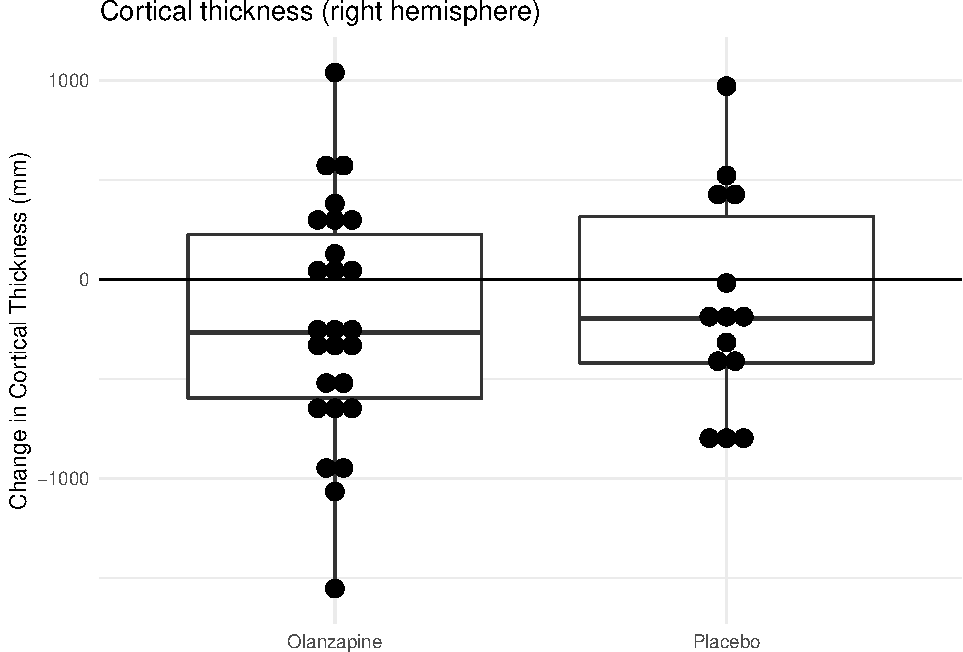
\includegraphics{07_STOPPD_CorticalSurfaceArea_byhemi_files/figure-latex/RCT_RSA_boxplot-1.pdf}

\begin{Shaded}
\begin{Highlighting}[]
\CommentTok{#boxplot of difference in thickness (y axis) by randomization group (x axis)}
\NormalTok{RCT_SA }\OperatorTok
\StringTok{  }\KeywordTok{gather}\NormalTok{(TCT, mm, LSurfArea_change, RSurfArea_change) }\OperatorTok
\StringTok{  }\KeywordTok{mutate}\NormalTok{(}\DataTypeTok{ThickChange =} \KeywordTok{factor}\NormalTok{(TCT, }\DataTypeTok{levels =} \KeywordTok{c}\NormalTok{(}\StringTok{"LSurfArea_change"}\NormalTok{, }\StringTok{"RSurfArea_change"}\NormalTok{),}
                              \DataTypeTok{labels =} \KeywordTok{c}\NormalTok{(}\StringTok{"Left Hemisphere"}\NormalTok{, }\StringTok{"Right Hemisphere"}\NormalTok{))) }\OperatorTok
\KeywordTok{ggplot}\NormalTok{(}\KeywordTok{aes}\NormalTok{(}\DataTypeTok{x=}\NormalTok{ RandomArm, }\DataTypeTok{y =}\NormalTok{ mm)) }\OperatorTok{+}\StringTok{ }
\StringTok{     }\KeywordTok{geom_boxplot}\NormalTok{(}\DataTypeTok{outlier.shape =} \OtherTok{NA}\NormalTok{) }\OperatorTok{+}\StringTok{ }
\StringTok{     }\KeywordTok{geom_dotplot}\NormalTok{(}\DataTypeTok{binaxis =} \StringTok{'y'}\NormalTok{, }\DataTypeTok{stackdir =} \StringTok{'center'}\NormalTok{) }\OperatorTok{+}
\StringTok{     }\KeywordTok{geom_hline}\NormalTok{(}\DataTypeTok{yintercept =} \DecValTok{0}\NormalTok{) }\OperatorTok{+}
\StringTok{     }\KeywordTok{labs}\NormalTok{(}\DataTypeTok{title =} \StringTok{"Change in Surface Area"}\NormalTok{,}\DataTypeTok{x =} \OtherTok{NULL}\NormalTok{, }\DataTypeTok{y =} \StringTok{"Change in Cortical Surface Area"}\NormalTok{) }\OperatorTok{+}
\StringTok{     }\KeywordTok{facet_wrap}\NormalTok{(}\OperatorTok{~}\StringTok{ }\NormalTok{ThickChange) }\OperatorTok{+}
\StringTok{     }\KeywordTok{theme_bw}\NormalTok{()}
\end{Highlighting}
\end{Shaded}

\begin{verbatim}
## `stat_bindot()` using `bins = 30`. Pick better value with `binwidth`.
\end{verbatim}

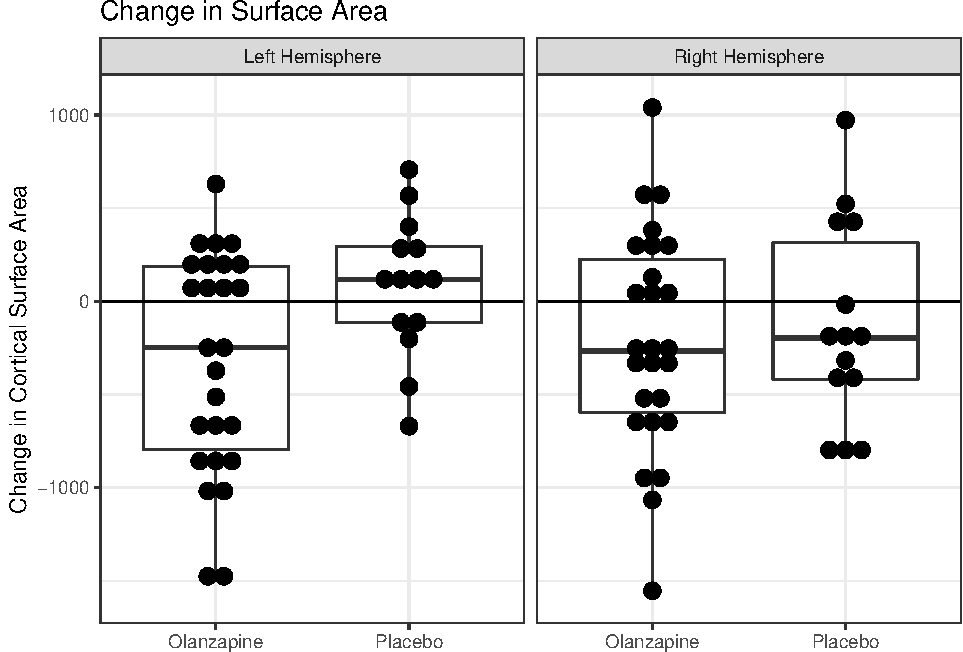
\includegraphics{07_STOPPD_CorticalSurfaceArea_byhemi_files/figure-latex/RCT_SA_facet_boxplot-1.pdf}

\begin{Shaded}
\begin{Highlighting}[]
\CommentTok{#run linear model without covariates}
\NormalTok{  fit_rct <-}\StringTok{ }\KeywordTok{lm}\NormalTok{(RSurfArea_change }\OperatorTok{~}\StringTok{ }\NormalTok{RandomArm, }\DataTypeTok{data=}\NormalTok{ RCT_SA)}
  \KeywordTok{print}\NormalTok{(fit_rct)}
\end{Highlighting}
\end{Shaded}

\begin{verbatim}
## 
## Call:
## lm(formula = RSurfArea_change ~ RandomArm, data = RCT_SA)
## 
## Coefficients:
##      (Intercept)  RandomArmPlacebo  
##          -215.28             90.53
\end{verbatim}

\begin{Shaded}
\begin{Highlighting}[]
  \KeywordTok{summary}\NormalTok{(fit_rct)}
\end{Highlighting}
\end{Shaded}

\begin{verbatim}
## 
## Call:
## lm(formula = RSurfArea_change ~ RandomArm, data = RCT_SA)
## 
## Residuals:
##      Min       1Q   Median       3Q      Max 
## -1338.22  -341.50   -63.29   476.45  1254.88 
## 
## Coefficients:
##                  Estimate Std. Error t value Pr(>|t|)  
## (Intercept)       -215.28     112.33  -1.916   0.0628 .
## RandomArmPlacebo    90.53     189.87   0.477   0.6363  
## ---
## Signif. codes:  0 '***' 0.001 '**' 0.01 '*' 0.05 '.' 0.1 ' ' 1
## 
## Residual standard error: 572.8 on 38 degrees of freedom
## Multiple R-squared:  0.005946,   Adjusted R-squared:  -0.02021 
## F-statistic: 0.2273 on 1 and 38 DF,  p-value: 0.6363
\end{verbatim}

\begin{Shaded}
\begin{Highlighting}[]
\CommentTok{#run linear model with covariates of sex and age}
\NormalTok{  fit_rct <-}\StringTok{ }\KeywordTok{lm}\NormalTok{(RSurfArea_change }\OperatorTok{~}\StringTok{ }\NormalTok{RandomArm }\OperatorTok{+}\StringTok{ }\NormalTok{sex }\OperatorTok{+}\StringTok{ }\NormalTok{age, }\DataTypeTok{data=}\NormalTok{ RCT_SA)}
  \KeywordTok{print}\NormalTok{(fit_rct)}
\end{Highlighting}
\end{Shaded}

\begin{verbatim}
## 
## Call:
## lm(formula = RSurfArea_change ~ RandomArm + sex + age, data = RCT_SA)
## 
## Coefficients:
##      (Intercept)  RandomArmPlacebo              sexM               age  
##          205.920           143.174           153.063            -9.417
\end{verbatim}

\begin{Shaded}
\begin{Highlighting}[]
  \KeywordTok{summary}\NormalTok{(fit_rct)}
\end{Highlighting}
\end{Shaded}

\begin{verbatim}
## 
## Call:
## lm(formula = RSurfArea_change ~ RandomArm + sex + age, data = RCT_SA)
## 
## Residuals:
##      Min       1Q   Median       3Q      Max 
## -1168.56  -430.29   -71.21   390.09  1433.95 
## 
## Coefficients:
##                  Estimate Std. Error t value Pr(>|t|)
## (Intercept)       205.920    358.036   0.575    0.569
## RandomArmPlacebo  143.174    192.356   0.744    0.462
## sexM              153.063    185.168   0.827    0.414
## age                -9.417      6.641  -1.418    0.165
## 
## Residual standard error: 570.4 on 36 degrees of freedom
## Multiple R-squared:  0.06603,    Adjusted R-squared:  -0.0118 
## F-statistic: 0.8484 on 3 and 36 DF,  p-value: 0.4766
\end{verbatim}

\begin{Shaded}
\begin{Highlighting}[]
\CommentTok{#run linear model with covariates of sex and age}
\NormalTok{  fit_rct <-}\StringTok{ }\KeywordTok{lm}\NormalTok{(RSurfArea_change }\OperatorTok{~}\StringTok{ }\NormalTok{RandomArm }\OperatorTok{+}\StringTok{ }\NormalTok{sex }\OperatorTok{+}\StringTok{ }\NormalTok{age }\OperatorTok{+}\StringTok{ }\NormalTok{site, }\DataTypeTok{data=}\NormalTok{ RCT_SA)}
  \KeywordTok{print}\NormalTok{(fit_rct)}
\end{Highlighting}
\end{Shaded}

\begin{verbatim}
## 
## Call:
## lm(formula = RSurfArea_change ~ RandomArm + sex + age + site, 
##     data = RCT_SA)
## 
## Coefficients:
##      (Intercept)  RandomArmPlacebo              sexM               age  
##           457.35            181.79            118.38            -15.16  
##          siteMAS           siteNKI           sitePMC  
##           -42.89            -40.79            523.20
\end{verbatim}

\begin{Shaded}
\begin{Highlighting}[]
  \KeywordTok{summary}\NormalTok{(fit_rct)}
\end{Highlighting}
\end{Shaded}

\begin{verbatim}
## 
## Call:
## lm(formula = RSurfArea_change ~ RandomArm + sex + age + site, 
##     data = RCT_SA)
## 
## Residuals:
##      Min       1Q   Median       3Q      Max 
## -1019.99  -393.21   -12.28   387.01  1153.36 
## 
## Coefficients:
##                  Estimate Std. Error t value Pr(>|t|)  
## (Intercept)       457.345    396.183   1.154   0.2566  
## RandomArmPlacebo  181.787    193.718   0.938   0.3549  
## sexM              118.375    185.840   0.637   0.5285  
## age               -15.158      7.234  -2.095   0.0439 *
## siteMAS           -42.885    247.049  -0.174   0.8632  
## siteNKI           -40.794    236.098  -0.173   0.8639  
## sitePMC           523.197    290.050   1.804   0.0804 .
## ---
## Signif. codes:  0 '***' 0.001 '**' 0.01 '*' 0.05 '.' 0.1 ' ' 1
## 
## Residual standard error: 563.5 on 33 degrees of freedom
## Multiple R-squared:  0.1646, Adjusted R-squared:  0.0127 
## F-statistic: 1.084 on 6 and 33 DF,  p-value: 0.3924
\end{verbatim}

\subsection{RCT \& Relapse (with time as
factor)}\label{rct-relapse-with-time-as-factor-1}

\begin{Shaded}
\begin{Highlighting}[]
\CommentTok{#restructure data for RCT & Relapse participants (N=72)}
\NormalTok{  RCTRelapse_LSA <-}\StringTok{ }\NormalTok{df }\OperatorTok
\StringTok{    }\KeywordTok{gather}\NormalTok{(oldcolname, SurfArea, LSurfArea_}\DecValTok{01}\NormalTok{, LSurfArea_}\DecValTok{02}\NormalTok{) }\OperatorTok
\StringTok{    }\KeywordTok{mutate}\NormalTok{(}\DataTypeTok{model_days =} \KeywordTok{if_else}\NormalTok{(oldcolname }\OperatorTok{==}\StringTok{ "LSurfArea_01"}\NormalTok{, }\DecValTok{1}\NormalTok{, dateDiff))}

\NormalTok{RCTRelapse_LSA }\OperatorTok\StringTok{ }\KeywordTok{filter}\NormalTok{(model_days }\OperatorTok{==}\StringTok{ }\DecValTok{1}\NormalTok{) }\OperatorTok\StringTok{ }\KeywordTok{count}\NormalTok{(randomization) }\OperatorTok\StringTok{ }\NormalTok{knitr}\OperatorTok{::}\KeywordTok{kable}\NormalTok{() }
\end{Highlighting}
\end{Shaded}

\begin{tabular}{l|r}
\hline
randomization & n\\
\hline
O & 38\\
\hline
P & 34\\
\hline
\end{tabular}

\begin{Shaded}
\begin{Highlighting}[]
\CommentTok{#plot all data, including outlier (participant 210030)}
\NormalTok{  RCTRelapse_LSA }\OperatorTok
\StringTok{   }\KeywordTok{ggplot}\NormalTok{(}\KeywordTok{aes}\NormalTok{(}\DataTypeTok{x=}\NormalTok{model_days, }\DataTypeTok{y=}\NormalTok{SurfArea, }\DataTypeTok{colour=}\NormalTok{RandomArm)) }\OperatorTok{+}\StringTok{ }
\StringTok{   }\KeywordTok{geom_point}\NormalTok{() }\OperatorTok{+}\StringTok{ }
\StringTok{   }\KeywordTok{geom_line}\NormalTok{(}\KeywordTok{aes}\NormalTok{(}\DataTypeTok{group=}\NormalTok{STUDYID), }\DataTypeTok{alpha =} \FloatTok{0.5}\NormalTok{) }\OperatorTok{+}\StringTok{ }
\StringTok{   }\KeywordTok{geom_smooth}\NormalTok{(}\DataTypeTok{method=}\StringTok{"lm"}\NormalTok{, }\DataTypeTok{formula=}\NormalTok{y}\OperatorTok{~}\KeywordTok{poly}\NormalTok{(x,}\DecValTok{1}\NormalTok{)) }\OperatorTok{+}
\StringTok{   }\KeywordTok{ggtitle}\NormalTok{(}\StringTok{"Surface Area in left hemisphere over time"}\NormalTok{) }\OperatorTok{+}
\StringTok{   }\KeywordTok{labs}\NormalTok{(}\DataTypeTok{x =} \StringTok{"Days between MRIs"}\NormalTok{, }\DataTypeTok{y =} \StringTok{"Surface Area"}\NormalTok{, }\DataTypeTok{colour =} \OtherTok{NULL}\NormalTok{) }\OperatorTok{+}
\StringTok{   }\KeywordTok{theme_minimal}\NormalTok{()}
\end{Highlighting}
\end{Shaded}

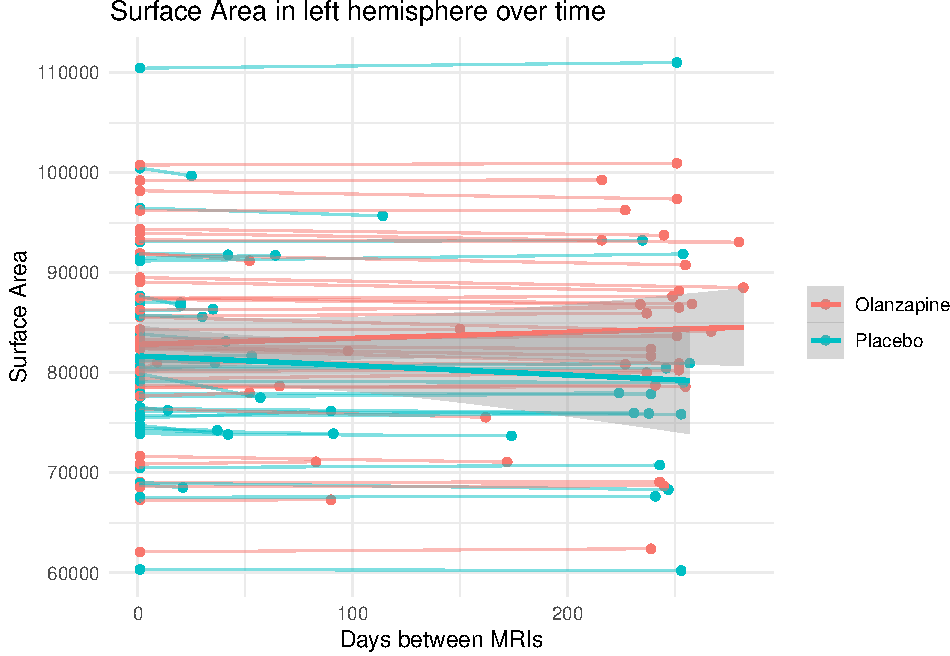
\includegraphics{07_STOPPD_CorticalSurfaceArea_byhemi_files/figure-latex/RCTRelapse_LSA_plot-1.pdf}

\begin{Shaded}
\begin{Highlighting}[]
\CommentTok{#run mixed linear model, with covariates}
\NormalTok{  fit_all <-}\StringTok{ }\KeywordTok{lmer}\NormalTok{(SurfArea }\OperatorTok{~}\StringTok{ }\NormalTok{RandomArm}\OperatorTok{*}\NormalTok{model_days }\OperatorTok{+}\StringTok{ }\NormalTok{sex }\OperatorTok{+}\StringTok{ }\NormalTok{age }\OperatorTok{+}\StringTok{ }\NormalTok{(}\DecValTok{1}\OperatorTok{|}\NormalTok{STUDYID), }\DataTypeTok{data=}\NormalTok{ RCTRelapse_LSA)}
  \KeywordTok{summary}\NormalTok{(fit_all)}
\end{Highlighting}
\end{Shaded}

\begin{verbatim}
## Linear mixed model fit by REML. t-tests use Satterthwaite's method [
## lmerModLmerTest]
## Formula: SurfArea ~ RandomArm * model_days + sex + age + (1 | STUDYID)
##    Data: RCTRelapse_LSA
## 
## REML criterion at convergence: 2546.9
## 
## Scaled residuals: 
##      Min       1Q   Median       3Q      Max 
## -2.93057 -0.46073 -0.01316  0.45586  2.94909 
## 
## Random effects:
##  Groups   Name        Variance Std.Dev.
##  STUDYID  (Intercept) 60349627 7768.5  
##  Residual               163892  404.8  
## Number of obs: 144, groups:  STUDYID, 72
## 
## Fixed effects:
##                               Estimate Std. Error         df t value
## (Intercept)                 83706.3319  3576.7100    68.0230  23.403
## RandomArmPlacebo            -2037.5203  1839.8200    68.1405  -1.107
## model_days                     -1.2902     0.4267    70.0200  -3.024
## sexM                        11595.6870  1845.3747    67.9977   6.284
## age                          -102.3534    60.2578    67.9978  -1.699
## RandomArmPlacebo:model_days     1.2418     0.7210    70.0491   1.722
##                             Pr(>|t|)    
## (Intercept)                  < 2e-16 ***
## RandomArmPlacebo             0.27199    
## model_days                   0.00349 ** 
## sexM                         2.7e-08 ***
## age                          0.09397 .  
## RandomArmPlacebo:model_days  0.08943 .  
## ---
## Signif. codes:  0 '***' 0.001 '**' 0.01 '*' 0.05 '.' 0.1 ' ' 1
## 
## Correlation of Fixed Effects:
##             (Intr) RndmAP mdl_dy sexM   age   
## RndmArmPlcb -0.201                            
## model_days  -0.014  0.024                     
## sexM        -0.172  0.037  0.000              
## age         -0.903 -0.055  0.001 -0.079       
## RndmArmPl:_  0.008 -0.032 -0.592  0.001  0.000
\end{verbatim}

\begin{Shaded}
\begin{Highlighting}[]
\CommentTok{#run mixed linear model, with covariates}
\NormalTok{  fit_all <-}\StringTok{ }\KeywordTok{lmer}\NormalTok{(SurfArea }\OperatorTok{~}\StringTok{ }\NormalTok{RandomArm}\OperatorTok{*}\NormalTok{model_days }\OperatorTok{+}\StringTok{ }\NormalTok{sex }\OperatorTok{+}\StringTok{ }\NormalTok{age }\OperatorTok{+}\StringTok{ }\NormalTok{site }\OperatorTok{+}\StringTok{ }\NormalTok{(}\DecValTok{1}\OperatorTok{|}\NormalTok{STUDYID), }\DataTypeTok{data=}\NormalTok{ RCTRelapse_LSA)}
  \KeywordTok{summary}\NormalTok{(fit_all)}
\end{Highlighting}
\end{Shaded}

\begin{verbatim}
## Linear mixed model fit by REML. t-tests use Satterthwaite's method [
## lmerModLmerTest]
## Formula: 
## SurfArea ~ RandomArm * model_days + sex + age + site + (1 | STUDYID)
##    Data: RCTRelapse_LSA
## 
## REML criterion at convergence: 2482.9
## 
## Scaled residuals: 
##      Min       1Q   Median       3Q      Max 
## -2.95470 -0.46259 -0.00638  0.45970  2.92462 
## 
## Random effects:
##  Groups   Name        Variance Std.Dev.
##  STUDYID  (Intercept) 52724012 7261.1  
##  Residual               163892  404.8  
## Number of obs: 144, groups:  STUDYID, 72
## 
## Fixed effects:
##                               Estimate Std. Error         df t value
## (Intercept)                 84101.9412  3509.6531    65.0236  23.963
## RandomArmPlacebo            -2019.4088  1744.0368    65.1500  -1.158
## model_days                     -1.2904     0.4267    70.0215  -3.024
## sexM                        10935.7319  1748.4462    64.9973   6.255
## age                          -118.5383    56.7389    64.9976  -2.089
## siteMAS                     -2376.9627  2218.6137    64.9977  -1.071
## siteNKI                      1074.8893  2458.6459    64.9977   0.437
## sitePMC                      7182.3728  2529.8337    64.9972   2.839
## RandomArmPlacebo:model_days     1.2397     0.7210    70.0557   1.719
##                             Pr(>|t|)    
## (Intercept)                  < 2e-16 ***
## RandomArmPlacebo             0.25113    
## model_days                   0.00348 ** 
## sexM                        3.52e-08 ***
## age                          0.04061 *  
## siteMAS                      0.28796    
## siteNKI                      0.66342    
## sitePMC                      0.00603 ** 
## RandomArmPlacebo:model_days  0.08997 .  
## ---
## Signif. codes:  0 '***' 0.001 '**' 0.01 '*' 0.05 '.' 0.1 ' ' 1
## 
## Correlation of Fixed Effects:
##             (Intr) RndmAP mdl_dy sexM   age    sitMAS sitNKI sitPMC
## RndmArmPlcb -0.139                                                 
## model_days  -0.014  0.025                                          
## sexM        -0.130  0.055  0.000                                   
## age         -0.882 -0.066  0.002 -0.076                            
## siteMAS     -0.292 -0.147  0.002 -0.066  0.108                     
## siteNKI     -0.175 -0.119 -0.002 -0.119  0.010  0.357              
## sitePMC     -0.153 -0.089  0.000 -0.144 -0.009  0.343  0.319       
## RndmArmPl:_  0.008 -0.034 -0.592  0.001 -0.001  0.000  0.002  0.000
\end{verbatim}

\subsubsection{Running the right hemisphere
RCTRelapse}\label{running-the-right-hemisphere-rctrelapse-1}

\begin{Shaded}
\begin{Highlighting}[]
\CommentTok{#restructure data for RCT & Relapse participants (N=72)}
\NormalTok{  RCTRelapse_RSA <-}\StringTok{ }\NormalTok{df }\OperatorTok
\StringTok{    }\KeywordTok{gather}\NormalTok{(oldcolname, SurfArea, RSurfArea_}\DecValTok{01}\NormalTok{, RSurfArea_}\DecValTok{02}\NormalTok{) }\OperatorTok
\StringTok{    }\KeywordTok{mutate}\NormalTok{(}\DataTypeTok{model_days =} \KeywordTok{if_else}\NormalTok{(oldcolname }\OperatorTok{==}\StringTok{ "RSurfArea_01"}\NormalTok{, }\DecValTok{1}\NormalTok{, dateDiff))}

\CommentTok{#plot all data, including outlier (participant 210030)}
\NormalTok{  RCTRelapse_RSA }\OperatorTok
\StringTok{   }\KeywordTok{ggplot}\NormalTok{(}\KeywordTok{aes}\NormalTok{(}\DataTypeTok{x=}\NormalTok{model_days, }\DataTypeTok{y=}\NormalTok{SurfArea, }\DataTypeTok{colour=}\NormalTok{RandomArm)) }\OperatorTok{+}\StringTok{ }
\StringTok{   }\KeywordTok{geom_point}\NormalTok{() }\OperatorTok{+}\StringTok{ }
\StringTok{   }\KeywordTok{geom_line}\NormalTok{(}\KeywordTok{aes}\NormalTok{(}\DataTypeTok{group=}\NormalTok{STUDYID), }\DataTypeTok{alpha =} \FloatTok{0.5}\NormalTok{) }\OperatorTok{+}\StringTok{ }
\StringTok{   }\KeywordTok{geom_smooth}\NormalTok{(}\DataTypeTok{method=}\StringTok{"lm"}\NormalTok{, }\DataTypeTok{formula=}\NormalTok{y}\OperatorTok{~}\KeywordTok{poly}\NormalTok{(x,}\DecValTok{1}\NormalTok{)) }\OperatorTok{+}
\StringTok{   }\KeywordTok{ggtitle}\NormalTok{(}\StringTok{"Surface Area in right hemisphere over time"}\NormalTok{) }\OperatorTok{+}
\StringTok{   }\KeywordTok{labs}\NormalTok{(}\DataTypeTok{x =} \StringTok{"Days between MRIs"}\NormalTok{, }\DataTypeTok{y =} \StringTok{"Surface Area"}\NormalTok{, }\DataTypeTok{colour =} \OtherTok{NULL}\NormalTok{) }\OperatorTok{+}
\StringTok{   }\KeywordTok{theme_minimal}\NormalTok{()}
\end{Highlighting}
\end{Shaded}

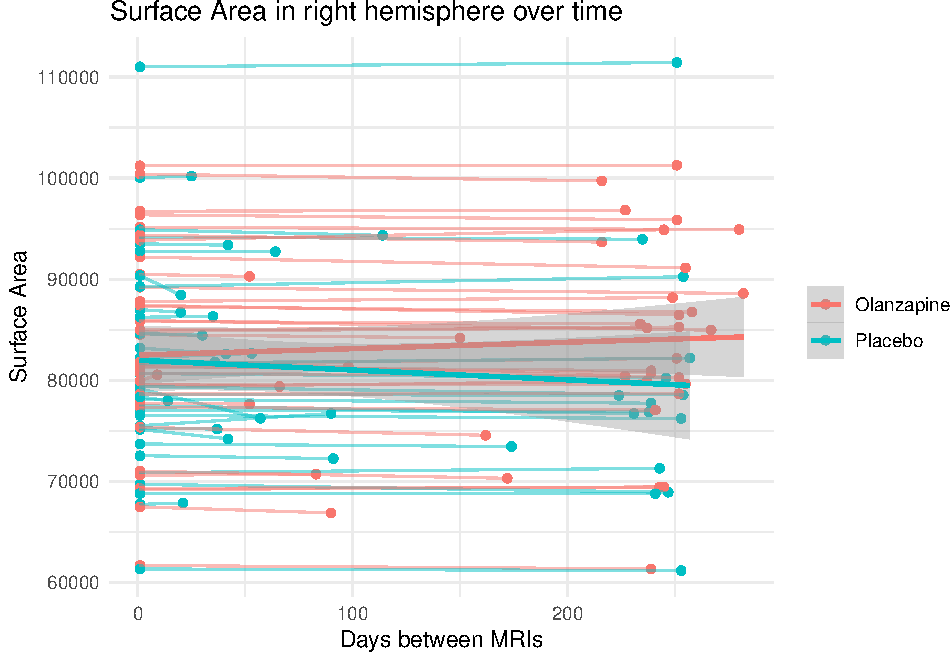
\includegraphics{07_STOPPD_CorticalSurfaceArea_byhemi_files/figure-latex/RCTRelapse_RSA_plot-1.pdf}

\begin{Shaded}
\begin{Highlighting}[]
\CommentTok{#run mixed linear model, with covariates}
\NormalTok{  fit_all <-}\StringTok{ }\KeywordTok{lmer}\NormalTok{(SurfArea }\OperatorTok{~}\StringTok{ }\NormalTok{RandomArm}\OperatorTok{*}\NormalTok{model_days }\OperatorTok{+}\StringTok{ }\NormalTok{sex }\OperatorTok{+}\StringTok{ }\NormalTok{age }\OperatorTok{+}\StringTok{ }\NormalTok{(}\DecValTok{1}\OperatorTok{|}\NormalTok{STUDYID), }\DataTypeTok{data=}\NormalTok{ RCTRelapse_RSA)}
  \KeywordTok{summary}\NormalTok{(fit_all)}
\end{Highlighting}
\end{Shaded}

\begin{verbatim}
## Linear mixed model fit by REML. t-tests use Satterthwaite's method [
## lmerModLmerTest]
## Formula: SurfArea ~ RandomArm * model_days + sex + age + (1 | STUDYID)
##    Data: RCTRelapse_RSA
## 
## REML criterion at convergence: 2567.1
## 
## Scaled residuals: 
##     Min      1Q  Median      3Q     Max 
## -3.1080 -0.3529 -0.0027  0.3822  3.1187 
## 
## Random effects:
##  Groups   Name        Variance Std.Dev.
##  STUDYID  (Intercept) 61430078 7837.7  
##  Residual               214731  463.4  
## Number of obs: 144, groups:  STUDYID, 72
## 
## Fixed effects:
##                               Estimate Std. Error         df t value
## (Intercept)                 83306.0885  3609.3846    68.0297  23.080
## RandomArmPlacebo            -1357.7075  1856.8569    68.1809  -0.731
## model_days                     -1.0748     0.4884    70.0260  -2.201
## sexM                        11573.0016  1862.1832    67.9972   6.215
## age                          -101.0096    60.8067    67.9974  -1.661
## RandomArmPlacebo:model_days     0.3065     0.8253    70.0634   0.371
##                             Pr(>|t|)    
## (Intercept)                  < 2e-16 ***
## RandomArmPlacebo              0.4672    
## model_days                    0.0311 *  
## sexM                        3.57e-08 ***
## age                           0.1013    
## RandomArmPlacebo:model_days   0.7114    
## ---
## Signif. codes:  0 '***' 0.001 '**' 0.01 '*' 0.05 '.' 0.1 ' ' 1
## 
## Correlation of Fixed Effects:
##             (Intr) RndmAP mdl_dy sexM   age   
## RndmArmPlcb -0.201                            
## model_days  -0.016  0.027                     
## sexM        -0.172  0.037  0.000              
## age         -0.903 -0.055  0.002 -0.079       
## RndmArmPl:_  0.009 -0.036 -0.592  0.001 -0.001
\end{verbatim}

\begin{Shaded}
\begin{Highlighting}[]
\CommentTok{#run mixed linear model, with covariates}
\NormalTok{  fit_all <-}\StringTok{ }\KeywordTok{lmer}\NormalTok{(SurfArea }\OperatorTok{~}\StringTok{ }\NormalTok{RandomArm}\OperatorTok{*}\NormalTok{model_days }\OperatorTok{+}\StringTok{ }\NormalTok{sex }\OperatorTok{+}\StringTok{ }\NormalTok{age }\OperatorTok{+}\StringTok{ }\NormalTok{site }\OperatorTok{+}\StringTok{ }\NormalTok{(}\DecValTok{1}\OperatorTok{|}\NormalTok{STUDYID), }\DataTypeTok{data=}\NormalTok{ RCTRelapse_RSA)}
  \KeywordTok{summary}\NormalTok{(fit_all)}
\end{Highlighting}
\end{Shaded}

\begin{verbatim}
## Linear mixed model fit by REML. t-tests use Satterthwaite's method [
## lmerModLmerTest]
## Formula: 
## SurfArea ~ RandomArm * model_days + sex + age + site + (1 | STUDYID)
##    Data: RCTRelapse_RSA
## 
## REML criterion at convergence: 2503.7
## 
## Scaled residuals: 
##      Min       1Q   Median       3Q      Max 
## -3.13482 -0.35071  0.00312  0.37950  3.09151 
## 
## Random effects:
##  Groups   Name        Variance Std.Dev.
##  STUDYID  (Intercept) 54283287 7367.7  
##  Residual               214731  463.4  
## Number of obs: 144, groups:  STUDYID, 72
## 
## Fixed effects:
##                               Estimate Std. Error         df t value
## (Intercept)                 83705.9315  3562.0240    65.0303  23.500
## RandomArmPlacebo            -1340.1774  1770.2952    65.1912  -0.757
## model_days                     -1.0753     0.4884    70.0277  -2.202
## sexM                        10923.1943  1774.4877    64.9969   6.156
## age                          -117.0597    57.5840    64.9973  -2.033
## siteMAS                     -2383.7886  2251.6589    64.9974  -1.059
## siteNKI                      1177.5286  2495.2662    64.9974   0.472
## sitePMC                      6985.0155  2567.5131    64.9968   2.721
## RandomArmPlacebo:model_days     0.3044     0.8253    70.0711   0.369
##                             Pr(>|t|)    
## (Intercept)                  < 2e-16 ***
## RandomArmPlacebo             0.45176    
## model_days                   0.03098 *  
## sexM                        5.22e-08 ***
## age                          0.04616 *  
## siteMAS                      0.29366    
## siteNKI                      0.63858    
## sitePMC                      0.00835 ** 
## RandomArmPlacebo:model_days  0.71338    
## ---
## Signif. codes:  0 '***' 0.001 '**' 0.01 '*' 0.05 '.' 0.1 ' ' 1
## 
## Correlation of Fixed Effects:
##             (Intr) RndmAP mdl_dy sexM   age    sitMAS sitNKI sitPMC
## RndmArmPlcb -0.139                                                 
## model_days  -0.016  0.028                                          
## sexM        -0.130  0.055  0.000                                   
## age         -0.882 -0.066  0.002 -0.076                            
## siteMAS     -0.292 -0.147  0.002 -0.066  0.108                     
## siteNKI     -0.175 -0.119 -0.002 -0.119  0.010  0.357              
## sitePMC     -0.153 -0.089  0.000 -0.144 -0.009  0.343  0.319       
## RndmArmPl:_  0.009 -0.038 -0.592  0.001 -0.001  0.000  0.002  0.000
\end{verbatim}

\subsection{Dealing with the
confusion..}\label{dealing-with-the-confusion..}

So I (maybe for one) Was Confused by the way that the two findings above
seems to go in opposite directions.

I.e. More the RCT analysis shows a decrease in surface area with
Olanzapine, while the longitudinal fit is trending upward.

I thought it might be useful to rebuild the first plot, but with the
whole sample, with point color representing the time between scans

Note that the dark blue dots would be the one's included in the RCT
analysis

\begin{Shaded}
\begin{Highlighting}[]
\CommentTok{#boxplot of difference in thickness (y axis) by randomization group (x axis)}
\NormalTok{df }\OperatorTok
\StringTok{  }\KeywordTok{gather}\NormalTok{(TCT, mm, LSurfArea_change, RSurfArea_change) }\OperatorTok
\StringTok{  }\KeywordTok{mutate}\NormalTok{(}\DataTypeTok{ThickChange =} \KeywordTok{factor}\NormalTok{(TCT, }\DataTypeTok{levels =} \KeywordTok{c}\NormalTok{(}\StringTok{"LSurfArea_change"}\NormalTok{, }\StringTok{"RSurfArea_change"}\NormalTok{),}
                              \DataTypeTok{labels =} \KeywordTok{c}\NormalTok{(}\StringTok{"Left Hemisphere"}\NormalTok{, }\StringTok{"Right Hemisphere"}\NormalTok{))) }\OperatorTok
\KeywordTok{ggplot}\NormalTok{(}\KeywordTok{aes}\NormalTok{(}\DataTypeTok{x=}\NormalTok{ RandomArm, }\DataTypeTok{y =}\NormalTok{ mm)) }\OperatorTok{+}\StringTok{ }
\StringTok{     }\KeywordTok{geom_boxplot}\NormalTok{(}\DataTypeTok{outlier.shape =} \OtherTok{NA}\NormalTok{) }\OperatorTok{+}\StringTok{ }
\StringTok{     }\KeywordTok{geom_jitter}\NormalTok{(}\KeywordTok{aes}\NormalTok{(}\DataTypeTok{color =}\NormalTok{ dateDiff)) }\OperatorTok{+}
\StringTok{     }\KeywordTok{geom_hline}\NormalTok{(}\DataTypeTok{yintercept =} \DecValTok{0}\NormalTok{) }\OperatorTok{+}
\StringTok{     }\KeywordTok{labs}\NormalTok{(}\DataTypeTok{title =} \StringTok{"Change in Surface Area"}\NormalTok{,}\DataTypeTok{x =} \OtherTok{NULL}\NormalTok{, }\DataTypeTok{y =} \StringTok{"Change in Cortical Surface Area"}\NormalTok{) }\OperatorTok{+}
\StringTok{     }\KeywordTok{facet_wrap}\NormalTok{(}\OperatorTok{~}\StringTok{ }\NormalTok{ThickChange) }\OperatorTok{+}
\StringTok{     }\KeywordTok{scale_color_viridis_c}\NormalTok{(}\DataTypeTok{direction =} \OperatorTok{-}\DecValTok{1}\NormalTok{) }\OperatorTok{+}
\StringTok{     }\KeywordTok{theme_bw}\NormalTok{()}
\end{Highlighting}
\end{Shaded}

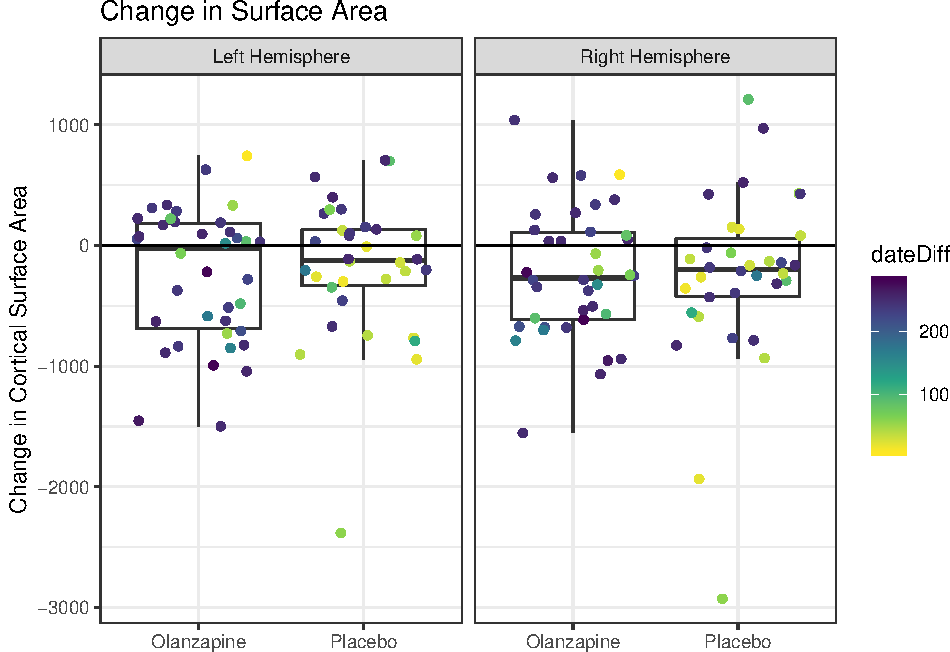
\includegraphics{07_STOPPD_CorticalSurfaceArea_byhemi_files/figure-latex/RCTRelapse_SA_facet_boxplot-1.pdf}

\section{Whole Skeleton Fractional
Anisotropy}\label{whole-skeleton-fractional-anisotropy}

\begin{Shaded}
\begin{Highlighting}[]
\CommentTok{#load libraries}
\KeywordTok{library}\NormalTok{(tidyverse)}
\KeywordTok{library}\NormalTok{(lme4)}
\KeywordTok{library}\NormalTok{(lmerTest)}
\KeywordTok{library}\NormalTok{(growthmodels)}
\end{Highlighting}
\end{Shaded}

\begin{Shaded}
\begin{Highlighting}[]
\CommentTok{#bring in subject info (generated by 03_STOPPD_masterDF.Rmd)}
\CommentTok{# then take only the subjects who completed (n= 72 - note two were excluded for IF)}
\NormalTok{df <-}\StringTok{ }\KeywordTok{read_csv}\NormalTok{(}\StringTok{'../generated_csvs/STOPPD_masterDF_2018-11-05.csv'}\NormalTok{) }\OperatorTok
\StringTok{  }\KeywordTok{mutate}\NormalTok{(}\DataTypeTok{STUDYID =} \KeywordTok{as.character}\NormalTok{(STUDYID)) }\OperatorTok
\StringTok{  }\KeywordTok{filter}\NormalTok{(second_complete }\OperatorTok{==}\StringTok{ "Yes"}\NormalTok{, MR_exclusion }\OperatorTok{==}\StringTok{ "No"}\NormalTok{) }

\CommentTok{#rename timepoint variable for clarity}
\KeywordTok{colnames}\NormalTok{(df)[}\KeywordTok{colnames}\NormalTok{(df)}\OperatorTok{==}\StringTok{"second_timepoint"}\NormalTok{] <-}\StringTok{ "category"} 

\CommentTok{#make a datediff column for time between scans}
\NormalTok{df}\OperatorTok{$}\NormalTok{dateDiff <-}\StringTok{ }\KeywordTok{as.numeric}\NormalTok{(}\KeywordTok{round}\NormalTok{(}\KeywordTok{difftime}\NormalTok{(df}\OperatorTok{$}\NormalTok{second_date, df}\OperatorTok{$}\NormalTok{first_date, }\DataTypeTok{units =} \StringTok{"days"}\NormalTok{), }\DecValTok{0}\NormalTok{))}
\end{Highlighting}
\end{Shaded}

\subsection{Known exclusion reasons}\label{known-exclusion-reasons}

\paragraph{known DWI issues}\label{known-dwi-issues}

\textbf{subject 410012 timepoint 02} -\textgreater{} scan was
blacklisted ``aborted'' for system failure..no DWI for this participant

\textbf{subject 220009\_timepoint 01} -\textgreater{} scan was also
incomplete (this participant was only able complete the T1w)

So we will filter the data table to exclude these 2 participants (final
n=71)

\begin{Shaded}
\begin{Highlighting}[]
\NormalTok{df <-}\StringTok{ }\KeywordTok{filter}\NormalTok{(df, }\OperatorTok{!}\NormalTok{(STUDYID }\OperatorTok\StringTok{ }\KeywordTok{c}\NormalTok{(}\StringTok{"410012"}\NormalTok{, }\StringTok{"220009"}\NormalTok{)))}
\end{Highlighting}
\end{Shaded}

\subsection{mangling the Mean Diffusivity cata
data}\label{mangling-the-mean-diffusivity-cata-data}

Erin reran the enigma DTI pipeline for only PMC using a different skull
stripping parameter (-fa 0.7 to BET). We will use these numbers instead
of the others in the archive here..

\begin{Shaded}
\begin{Highlighting}[]
\CommentTok{#bring in FA data (from the filesystem)}
\NormalTok{FA_most <-}\StringTok{ }\KeywordTok{read_csv}\NormalTok{(}\StringTok{'../data/enigma-DTI_archive_201811/enigmaDTI-FA-results.csv'}\NormalTok{)}
\NormalTok{FA_PMC <-}\StringTok{ }\KeywordTok{read_csv}\NormalTok{(}\StringTok{'../data/enigma-DTI_PMCredo_201809/enigmaDTI-FA-results.csv'}\NormalTok{)}

\CommentTok{# separate id into it's parts and then drop old PMC data}
\NormalTok{FA_most <-}\StringTok{ }\NormalTok{FA_most }\OperatorTok
\StringTok{  }\KeywordTok{separate}\NormalTok{(id, }\DataTypeTok{into =} \KeywordTok{c}\NormalTok{(}\StringTok{"study"}\NormalTok{, }\StringTok{"site"}\NormalTok{, }\StringTok{"STUDYID"}\NormalTok{, }\StringTok{"timepoint"}\NormalTok{)) }\OperatorTok
\StringTok{  }\KeywordTok{filter}\NormalTok{(site }\OperatorTok{!=}\StringTok{ "PMC"}\NormalTok{)}

\CommentTok{# separate the PMC subject id into it's parts and then bind to the data from the other sites }
\NormalTok{FA <-}\StringTok{ }\NormalTok{FA_PMC }\OperatorTok
\StringTok{  }\KeywordTok{separate}\NormalTok{(id, }\DataTypeTok{into =} \KeywordTok{c}\NormalTok{(}\StringTok{"study"}\NormalTok{, }\StringTok{"site"}\NormalTok{, }\StringTok{"STUDYID"}\NormalTok{, }\StringTok{"timepoint"}\NormalTok{)) }\OperatorTok
\StringTok{  }\KeywordTok{bind_rows}\NormalTok{(FA_most)}

\CommentTok{# drop acute ("00") and other ("03") timepoints from the analysis}
\NormalTok{FA <-}\StringTok{ }\NormalTok{FA }\OperatorTok\StringTok{ }
\StringTok{  }\KeywordTok{filter}\NormalTok{(}\OperatorTok{!}\NormalTok{(timepoint }\OperatorTok\StringTok{ }\KeywordTok{c}\NormalTok{(}\StringTok{"00"}\NormalTok{, }\StringTok{"03"}\NormalTok{))) }\OperatorTok
\StringTok{  }\KeywordTok{gather}\NormalTok{(tract, FA, }\KeywordTok{ends_with}\NormalTok{(}\StringTok{"FA"}\NormalTok{)) }\OperatorTok
\StringTok{  }\KeywordTok{unite}\NormalTok{(tract_timepoint, tract, timepoint) }\OperatorTok
\StringTok{  }\KeywordTok{spread}\NormalTok{(tract_timepoint, FA)}
\end{Highlighting}
\end{Shaded}

\subsection{check for missing FA data}\label{check-for-missing-fa-data}

\begin{Shaded}
\begin{Highlighting}[]
\CommentTok{# filter the master spreadsheet for the list of completers (no output means we are ok)}
\NormalTok{df }\OperatorTok
\StringTok{  }\KeywordTok{anti_join}\NormalTok{(FA, }\DataTypeTok{by =} \StringTok{"STUDYID"}\NormalTok{) }\OperatorTok
\StringTok{  }\KeywordTok{summarise}\NormalTok{(}\StringTok{`}\DataTypeTok{Number of missing FA values}\StringTok{`}\NormalTok{ =}\StringTok{ }\KeywordTok{n}\NormalTok{()) }\OperatorTok
\StringTok{  }\NormalTok{knitr}\OperatorTok{::}\KeywordTok{kable}\NormalTok{()}
\end{Highlighting}
\end{Shaded}

\begin{tabular}{r}
\hline
Number of missing FA values\\
\hline
0\\
\hline
\end{tabular}

\subsection{merge (i.e.~join) the FA data with the clinical
scores}\label{merge-i.e.join-the-fa-data-with-the-clinical-scores}

\begin{Shaded}
\begin{Highlighting}[]
\NormalTok{all_FA <-}\StringTok{ }\NormalTok{df }\OperatorTok
\StringTok{  }\KeywordTok{select}\NormalTok{(STUDYID, sex, age, randomization, category, dateDiff) }\OperatorTok
\StringTok{  }\KeywordTok{left_join}\NormalTok{(FA, }\DataTypeTok{by =} \StringTok{"STUDYID"}\NormalTok{)}

\NormalTok{all_FA }\OperatorTok
\StringTok{  }\KeywordTok{filter}\NormalTok{(}\KeywordTok{is.na}\NormalTok{(AverageFA_FA_}\DecValTok{01}\NormalTok{)) }\OperatorTok
\StringTok{  }\KeywordTok{summarise}\NormalTok{(}\StringTok{`}\DataTypeTok{Number of missing timepoint 1 FA values}\StringTok{`}\NormalTok{ =}\StringTok{ }\KeywordTok{n}\NormalTok{()) }\OperatorTok
\StringTok{  }\NormalTok{knitr}\OperatorTok{::}\KeywordTok{kable}\NormalTok{()}
\end{Highlighting}
\end{Shaded}

\begin{tabular}{r}
\hline
Number of missing timepoint 1 FA values\\
\hline
0\\
\hline
\end{tabular}

\begin{Shaded}
\begin{Highlighting}[]
\NormalTok{all_FA }\OperatorTok
\StringTok{  }\KeywordTok{filter}\NormalTok{(}\KeywordTok{is.na}\NormalTok{(AverageFA_FA_}\DecValTok{02}\NormalTok{)) }\OperatorTok
\StringTok{  }\KeywordTok{summarise}\NormalTok{(}\StringTok{`}\DataTypeTok{Number of missing timepoint 2 FA values}\StringTok{`}\NormalTok{ =}\StringTok{ }\KeywordTok{n}\NormalTok{()) }\OperatorTok
\StringTok{  }\NormalTok{knitr}\OperatorTok{::}\KeywordTok{kable}\NormalTok{()}
\end{Highlighting}
\end{Shaded}

\begin{tabular}{r}
\hline
Number of missing timepoint 2 FA values\\
\hline
0\\
\hline
\end{tabular}

\begin{Shaded}
\begin{Highlighting}[]
\CommentTok{#write out clean FA speadsheet (required for subsequent FA analyses)}
\KeywordTok{write.csv}\NormalTok{(all_FA, }\StringTok{'../generated_csvs/STOPPD_FAclean.csv'}\NormalTok{, }\DataTypeTok{row.names =} \OtherTok{FALSE}\NormalTok{)}
\end{Highlighting}
\end{Shaded}

\subsection{RCT only}\label{rct-only-2}

\begin{Shaded}
\begin{Highlighting}[]
\CommentTok{#boxplot of difference in FA in whole skeleton (y axis) by randomization group (x axis)}
\KeywordTok{ggplot}\NormalTok{(RCT_FA, }\KeywordTok{aes}\NormalTok{(}\DataTypeTok{x=}\NormalTok{ randomization, }\DataTypeTok{y =}\NormalTok{ diffAverageSkel_FA)) }\OperatorTok{+}\StringTok{ }
\StringTok{   }\KeywordTok{geom_boxplot}\NormalTok{(}\DataTypeTok{outlier.shape =} \OtherTok{NA}\NormalTok{) }\OperatorTok{+}\StringTok{ }
\StringTok{   }\KeywordTok{geom_dotplot}\NormalTok{(}\DataTypeTok{binaxis =} \StringTok{'y'}\NormalTok{, }\DataTypeTok{stackdir =} \StringTok{'center'}\NormalTok{) }\OperatorTok{+}
\StringTok{   }\KeywordTok{geom_hline}\NormalTok{(}\DataTypeTok{yintercept =} \DecValTok{0}\NormalTok{) }\OperatorTok{+}
\StringTok{   }\KeywordTok{ggtitle}\NormalTok{(}\StringTok{"Whole skeleton fractional anisotropy"}\NormalTok{) }\OperatorTok{+}
\StringTok{   }\KeywordTok{xlab}\NormalTok{(}\StringTok{"randomization condition"}\NormalTok{) }\OperatorTok{+}\StringTok{  }
\StringTok{   }\KeywordTok{ylab}\NormalTok{(}\StringTok{"difference between timepoints"}\NormalTok{) }\OperatorTok{+}
\StringTok{   }\KeywordTok{theme_minimal}\NormalTok{()}
\end{Highlighting}
\end{Shaded}

\begin{verbatim}
## `stat_bindot()` using `bins = 30`. Pick better value with `binwidth`.
\end{verbatim}

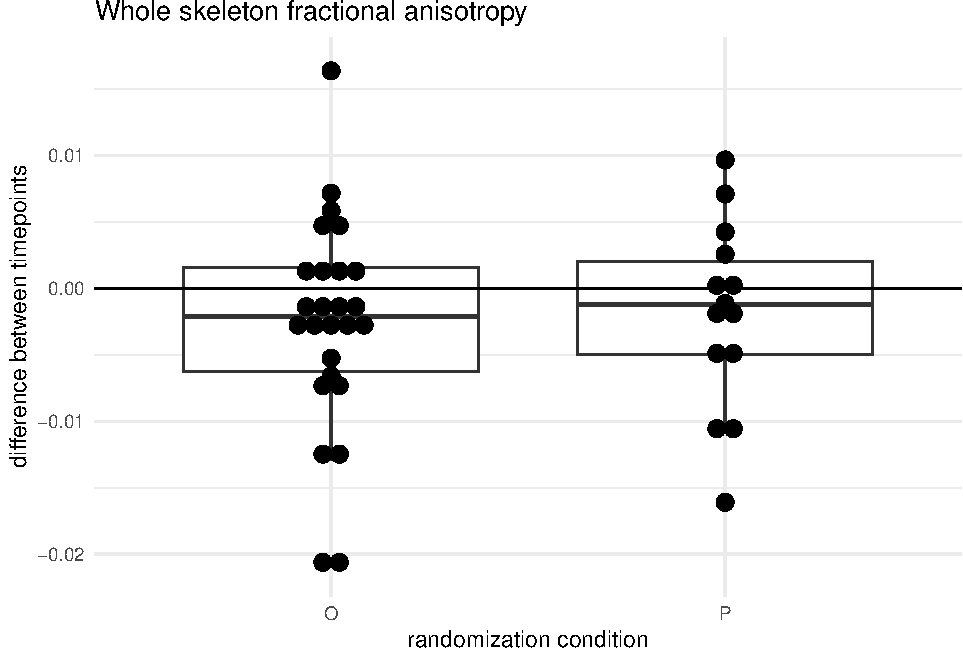
\includegraphics{08_STOPPD_FA-meanFAskel_files/figure-latex/RCT_FA_meanSkel_plot-1.pdf}

\begin{Shaded}
\begin{Highlighting}[]
\NormalTok{fit_rct <-}\StringTok{ }\KeywordTok{lm}\NormalTok{(diffAverageSkel_FA }\OperatorTok{~}\StringTok{ }\NormalTok{randomization, }\DataTypeTok{data=}\NormalTok{ RCT_FA)}
\KeywordTok{print}\NormalTok{(fit_rct)}
\end{Highlighting}
\end{Shaded}

\begin{verbatim}
## 
## Call:
## lm(formula = diffAverageSkel_FA ~ randomization, data = RCT_FA)
## 
## Coefficients:
##    (Intercept)  randomizationP  
##     -0.0026337       0.0006364
\end{verbatim}

\begin{Shaded}
\begin{Highlighting}[]
\KeywordTok{summary}\NormalTok{(fit_rct)}
\end{Highlighting}
\end{Shaded}

\begin{verbatim}
## 
## Call:
## lm(formula = diffAverageSkel_FA ~ randomization, data = RCT_FA)
## 
## Residuals:
##        Min         1Q     Median         3Q        Max 
## -0.0182273 -0.0032754  0.0007225  0.0043244  0.0190097 
## 
## Coefficients:
##                  Estimate Std. Error t value Pr(>|t|)  
## (Intercept)    -0.0026337  0.0015172  -1.736   0.0907 .
## randomizationP  0.0006364  0.0025645   0.248   0.8054  
## ---
## Signif. codes:  0 '***' 0.001 '**' 0.01 '*' 0.05 '.' 0.1 ' ' 1
## 
## Residual standard error: 0.007736 on 38 degrees of freedom
## Multiple R-squared:  0.001618,   Adjusted R-squared:  -0.02466 
## F-statistic: 0.06158 on 1 and 38 DF,  p-value: 0.8054
\end{verbatim}

\begin{Shaded}
\begin{Highlighting}[]
\CommentTok{#run linear model with covariates of sex and age}
\NormalTok{fit_rct <-}\StringTok{ }\KeywordTok{lm}\NormalTok{(diffAverageSkel_FA }\OperatorTok{~}\StringTok{ }\NormalTok{randomization }\OperatorTok{+}\StringTok{ }\NormalTok{sex }\OperatorTok{+}\StringTok{ }\NormalTok{age, }\DataTypeTok{data=}\NormalTok{ RCT_FA)}
\KeywordTok{print}\NormalTok{(fit_rct)}
\end{Highlighting}
\end{Shaded}

\begin{verbatim}
## 
## Call:
## lm(formula = diffAverageSkel_FA ~ randomization + sex + age, 
##     data = RCT_FA)
## 
## Coefficients:
##    (Intercept)  randomizationP            sexM             age  
##      0.0066641       0.0017724       0.0030420      -0.0002049
\end{verbatim}

\begin{Shaded}
\begin{Highlighting}[]
\KeywordTok{summary}\NormalTok{(fit_rct)}
\end{Highlighting}
\end{Shaded}

\begin{verbatim}
## 
## Call:
## lm(formula = diffAverageSkel_FA ~ randomization + sex + age, 
##     data = RCT_FA)
## 
## Residuals:
##        Min         1Q     Median         3Q        Max 
## -0.0176902 -0.0037512  0.0003699  0.0044837  0.0169146 
## 
## Coefficients:
##                   Estimate  Std. Error t value Pr(>|t|)  
## (Intercept)     0.00666412  0.00459470   1.450   0.1556  
## randomizationP  0.00177238  0.00246851   0.718   0.4774  
## sexM            0.00304198  0.00237628   1.280   0.2087  
## age            -0.00020489  0.00008522  -2.404   0.0215 *
## ---
## Signif. codes:  0 '***' 0.001 '**' 0.01 '*' 0.05 '.' 0.1 ' ' 1
## 
## Residual standard error: 0.00732 on 36 degrees of freedom
## Multiple R-squared:  0.1531, Adjusted R-squared:  0.08256 
## F-statistic:  2.17 on 3 and 36 DF,  p-value: 0.1085
\end{verbatim}

\begin{Shaded}
\begin{Highlighting}[]
\CommentTok{#run linear model with covariates of sex, age and site}
\NormalTok{fit_rct <-}\StringTok{ }\KeywordTok{lm}\NormalTok{(diffAverageSkel_FA }\OperatorTok{~}\StringTok{ }\NormalTok{randomization }\OperatorTok{+}\StringTok{ }\NormalTok{sex }\OperatorTok{+}\StringTok{ }\NormalTok{age }\OperatorTok{+}\StringTok{ }\NormalTok{site, }\DataTypeTok{data=}\NormalTok{ RCT_FA)}
\KeywordTok{print}\NormalTok{(fit_rct)}
\end{Highlighting}
\end{Shaded}

\begin{verbatim}
## 
## Call:
## lm(formula = diffAverageSkel_FA ~ randomization + sex + age + 
##     site, data = RCT_FA)
## 
## Coefficients:
##    (Intercept)  randomizationP            sexM             age  
##      0.0055312       0.0011892       0.0024924      -0.0002075  
##        siteMAS         siteNKI         sitePMC  
##      0.0048105       0.0015693       0.0027403
\end{verbatim}

\begin{Shaded}
\begin{Highlighting}[]
\KeywordTok{summary}\NormalTok{(fit_rct)}
\end{Highlighting}
\end{Shaded}

\begin{verbatim}
## 
## Call:
## lm(formula = diffAverageSkel_FA ~ randomization + sex + age + 
##     site, data = RCT_FA)
## 
## Residuals:
##        Min         1Q     Median         3Q        Max 
## -0.0164312 -0.0039600  0.0001338  0.0050820  0.0187285 
## 
## Coefficients:
##                   Estimate  Std. Error t value Pr(>|t|)  
## (Intercept)     0.00553120  0.00519594   1.065   0.2948  
## randomizationP  0.00118917  0.00254062   0.468   0.6428  
## sexM            0.00249237  0.00243729   1.023   0.3139  
## age            -0.00020752  0.00009488  -2.187   0.0359 *
## siteMAS         0.00481051  0.00324006   1.485   0.1471  
## siteNKI         0.00156932  0.00309643   0.507   0.6157  
## sitePMC         0.00274025  0.00380401   0.720   0.4764  
## ---
## Signif. codes:  0 '***' 0.001 '**' 0.01 '*' 0.05 '.' 0.1 ' ' 1
## 
## Residual standard error: 0.00739 on 33 degrees of freedom
## Multiple R-squared:  0.2089, Adjusted R-squared:  0.06501 
## F-statistic: 1.452 on 6 and 33 DF,  p-value: 0.2251
\end{verbatim}

\subsection{RCT \& Relapse (with time as
factor)}\label{rct-relapse-with-time-as-factor-2}

\begin{Shaded}
\begin{Highlighting}[]
\NormalTok{RCTRelapse_wholeskelFA <-}\StringTok{ }\NormalTok{RCTRelapse_FA }\OperatorTok
\StringTok{  }\KeywordTok{filter}\NormalTok{(Tract }\OperatorTok{==}\StringTok{ "AverageFA"}\NormalTok{)}
\CommentTok{#plot}
\NormalTok{RCTRelapse_wholeskelFA }\OperatorTok
\StringTok{  }\KeywordTok{ggplot}\NormalTok{(}\KeywordTok{aes}\NormalTok{(}\DataTypeTok{x=}\NormalTok{model_days, }\DataTypeTok{y=}\NormalTok{FA, }\DataTypeTok{colour=}\NormalTok{randomization)) }\OperatorTok{+}\StringTok{ }
\StringTok{  }\KeywordTok{geom_point}\NormalTok{() }\OperatorTok{+}\StringTok{ }
\StringTok{  }\KeywordTok{geom_line}\NormalTok{(}\KeywordTok{aes}\NormalTok{(}\DataTypeTok{group=}\NormalTok{STUDYID), }\DataTypeTok{alpha =} \FloatTok{0.5}\NormalTok{) }\OperatorTok{+}\StringTok{ }
\StringTok{  }\KeywordTok{geom_smooth}\NormalTok{(}\DataTypeTok{method=}\StringTok{"lm"}\NormalTok{, }\DataTypeTok{formula=}\NormalTok{y}\OperatorTok{~}\KeywordTok{poly}\NormalTok{(x,}\DecValTok{1}\NormalTok{)) }\OperatorTok{+}
\StringTok{  }\KeywordTok{ggtitle}\NormalTok{(}\StringTok{"Whole skeleton fractional anisotropy over time"}\NormalTok{) }\OperatorTok{+}\StringTok{    }
\StringTok{  }\KeywordTok{xlab}\NormalTok{(}\StringTok{"days between MRIs"}\NormalTok{) }\OperatorTok{+}\StringTok{  }
\StringTok{  }\KeywordTok{ylab}\NormalTok{(}\StringTok{"Mean Diffusivity"}\NormalTok{) }\OperatorTok{+}
\StringTok{  }\KeywordTok{theme_minimal}\NormalTok{()}
\end{Highlighting}
\end{Shaded}

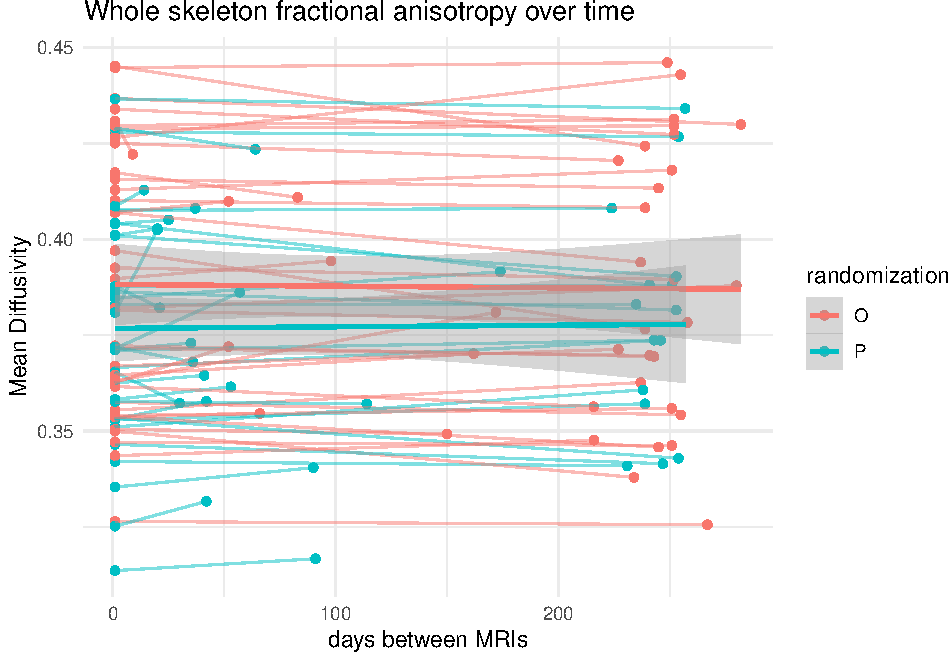
\includegraphics{08_STOPPD_FA-meanFAskel_files/figure-latex/RCTRelapse_FA_plot-1.pdf}

\begin{Shaded}
\begin{Highlighting}[]
\CommentTok{#run mixed linear model, with covariates}
\NormalTok{fit_all <-}\StringTok{ }\KeywordTok{lmer}\NormalTok{(FA }\OperatorTok{~}\StringTok{ }\NormalTok{randomization}\OperatorTok{*}\NormalTok{model_days }\OperatorTok{+}\StringTok{ }\NormalTok{sex }\OperatorTok{+}\StringTok{ }\NormalTok{age }\OperatorTok{+}\StringTok{ }\NormalTok{(}\DecValTok{1}\OperatorTok{|}\NormalTok{STUDYID), }\DataTypeTok{data=}\NormalTok{ RCTRelapse_wholeskelFA)}
\KeywordTok{summary}\NormalTok{(fit_all)}
\end{Highlighting}
\end{Shaded}

\begin{verbatim}
## Linear mixed model fit by REML. t-tests use Satterthwaite's method [
## lmerModLmerTest]
## Formula: FA ~ randomization * model_days + sex + age + (1 | STUDYID)
##    Data: RCTRelapse_wholeskelFA
## 
## REML criterion at convergence: -705.9
## 
## Scaled residuals: 
##      Min       1Q   Median       3Q      Max 
## -1.94972 -0.36140 -0.01493  0.37639  2.03848 
## 
## Random effects:
##  Groups   Name        Variance   Std.Dev.
##  STUDYID  (Intercept) 0.00091790 0.030297
##  Residual             0.00002934 0.005417
## Number of obs: 142, groups:  STUDYID, 71
## 
## Fixed effects:
##                               Estimate   Std. Error           df t value
## (Intercept)                0.420038504  0.014072666 67.294984696  29.848
## randomizationP            -0.010187596  0.007320306 68.631328224  -1.392
## model_days                -0.000006710  0.000005717 69.240746206  -1.174
## sexM                      -0.000889927  0.007300269 67.001340480  -0.122
## age                       -0.000570356  0.000237119 67.001860376  -2.405
## randomizationP:model_days  0.000002899  0.000009637 69.582543938   0.301
##                                      Pr(>|t|)    
## (Intercept)               <0.0000000000000002 ***
## randomizationP                         0.1685    
## model_days                             0.2446    
## sexM                                   0.9033    
## age                                    0.0189 *  
## randomizationP:model_days              0.7644    
## ---
## Signif. codes:  0 '***' 0.001 '**' 0.01 '*' 0.05 '.' 0.1 ' ' 1
## 
## Correlation of Fixed Effects:
##             (Intr) rndmzP mdl_dy sexM   age   
## randomiztnP -0.205                            
## model_days  -0.047  0.082                     
## sexM        -0.174  0.050  0.002              
## age         -0.899 -0.061  0.004 -0.085       
## rndmztnP:m_  0.026 -0.108 -0.593  0.002 -0.001
\end{verbatim}

\subsection{just wanna through in one site
model..}\label{just-wanna-through-in-one-site-model..}

\begin{Shaded}
\begin{Highlighting}[]
\CommentTok{#run mixed linear model, with covariates}
\NormalTok{fit_all <-}\StringTok{ }\KeywordTok{lmer}\NormalTok{(FA }\OperatorTok{~}\StringTok{ }\NormalTok{randomization}\OperatorTok{*}\NormalTok{model_days }\OperatorTok{+}\StringTok{ }\NormalTok{sex }\OperatorTok{+}\StringTok{ }\NormalTok{age }\OperatorTok{+}\StringTok{ }\NormalTok{site }\OperatorTok{+}\StringTok{ }\NormalTok{(}\DecValTok{1}\OperatorTok{|}\NormalTok{STUDYID), }\DataTypeTok{data=}\NormalTok{ RCTRelapse_wholeskelFA)}
\KeywordTok{summary}\NormalTok{(fit_all)}
\end{Highlighting}
\end{Shaded}

\begin{verbatim}
## Linear mixed model fit by REML. t-tests use Satterthwaite's method [
## lmerModLmerTest]
## Formula: 
## FA ~ randomization * model_days + sex + age + site + (1 | STUDYID)
##    Data: RCTRelapse_wholeskelFA
## 
## REML criterion at convergence: -763.4
## 
## Scaled residuals: 
##      Min       1Q   Median       3Q      Max 
## -2.22673 -0.36093  0.00773  0.40476  1.97403 
## 
## Random effects:
##  Groups   Name        Variance   Std.Dev.
##  STUDYID  (Intercept) 0.00026606 0.016311
##  Residual             0.00002933 0.005416
## Number of obs: 142, groups:  STUDYID, 71
## 
## Fixed effects:
##                               Estimate   Std. Error           df t value
## (Intercept)                0.446664113  0.008121600 64.854939100  54.997
## randomizationP            -0.001694241  0.004143105 68.953740506  -0.409
## model_days                -0.000006481  0.000005707 69.765390246  -1.136
## sexM                       0.007528548  0.004063003 64.002130344   1.853
## age                       -0.000644155  0.000131327 64.007125598  -4.905
## siteMAS                   -0.045128486  0.005245359 64.005598123  -8.604
## siteNKI                   -0.054431216  0.005671919 64.015089285  -9.597
## sitePMC                   -0.057667867  0.005835298 63.997753494  -9.883
## randomizationP:model_days  0.000002411  0.000009591 70.909497124   0.251
##                                       Pr(>|t|)    
## (Intercept)               < 0.0000000000000002 ***
## randomizationP                          0.6839    
## model_days                              0.2599    
## sexM                                    0.0685 .  
## age                         0.0000067266336686 ***
## siteMAS                     0.0000000000027939 ***
## siteNKI                     0.0000000000000519 ***
## sitePMC                     0.0000000000000168 ***
## randomizationP:model_days               0.8023    
## ---
## Signif. codes:  0 '***' 0.001 '**' 0.01 '*' 0.05 '.' 0.1 ' ' 1
## 
## Correlation of Fixed Effects:
##             (Intr) rndmzP mdl_dy sexM   age    sitMAS sitNKI sitPMC
## randomiztnP -0.141                                                 
## model_days  -0.082  0.144                                          
## sexM        -0.126  0.072  0.004                                   
## age         -0.878 -0.076  0.009 -0.086                            
## siteMAS     -0.290 -0.172  0.005 -0.092  0.124                     
## siteNKI     -0.175 -0.122 -0.011 -0.122  0.013  0.355              
## sitePMC     -0.153 -0.091 -0.001 -0.146 -0.007  0.341  0.320       
## rndmztnP:m_  0.044 -0.190 -0.595  0.002 -0.002  0.002  0.010  0.003
\end{verbatim}

\begin{Shaded}
\begin{Highlighting}[]
\CommentTok{#cleanup}
\KeywordTok{rm}\NormalTok{(}\StringTok{'df'}\NormalTok{, }\StringTok{'fit_all'}\NormalTok{, }\StringTok{'fit_rct'}\NormalTok{, }\StringTok{'FA'}\NormalTok{, }\StringTok{'plot'}\NormalTok{, }\StringTok{'RCT_FA'}\NormalTok{, }\StringTok{'RCTRelapse_FA'}\NormalTok{)}
\end{Highlighting}
\end{Shaded}

\begin{verbatim}
## Warning in rm("df", "fit_all", "fit_rct", "FA", "plot", "RCT_FA",
## "RCTRelapse_FA"): object 'plot' not found
\end{verbatim}

\section{Whole Skeleton Mean
Diffusivity}\label{whole-skeleton-mean-diffusivity}

\begin{Shaded}
\begin{Highlighting}[]
\CommentTok{#load libraries}
\KeywordTok{library}\NormalTok{(tidyverse)}
\KeywordTok{library}\NormalTok{(lme4)}
\KeywordTok{library}\NormalTok{(lmerTest)}
\KeywordTok{library}\NormalTok{(growthmodels)}
\end{Highlighting}
\end{Shaded}

\begin{Shaded}
\begin{Highlighting}[]
\CommentTok{#bring in subject info (generated by 03_STOPPD_masterDF.Rmd)}
\CommentTok{# then take only the subjects who completed (n= 72 - note two were excluded for IF)}
\NormalTok{df <-}\StringTok{ }\KeywordTok{read_csv}\NormalTok{(}\StringTok{'../generated_csvs/STOPPD_masterDF_2018-11-05.csv'}\NormalTok{) }\OperatorTok
\StringTok{  }\KeywordTok{mutate}\NormalTok{(}\DataTypeTok{STUDYID =} \KeywordTok{as.character}\NormalTok{(STUDYID)) }\OperatorTok
\StringTok{  }\KeywordTok{filter}\NormalTok{(second_complete }\OperatorTok{==}\StringTok{ "Yes"}\NormalTok{, MR_exclusion }\OperatorTok{==}\StringTok{ "No"}\NormalTok{) }

\CommentTok{#rename timepoint variable for clarity}
\KeywordTok{colnames}\NormalTok{(df)[}\KeywordTok{colnames}\NormalTok{(df)}\OperatorTok{==}\StringTok{"second_timepoint"}\NormalTok{] <-}\StringTok{ "category"} 

\CommentTok{#make a datediff column for time between scans}
\NormalTok{df}\OperatorTok{$}\NormalTok{dateDiff <-}\StringTok{ }\KeywordTok{as.numeric}\NormalTok{(}\KeywordTok{round}\NormalTok{(}\KeywordTok{difftime}\NormalTok{(df}\OperatorTok{$}\NormalTok{second_date, df}\OperatorTok{$}\NormalTok{first_date, }\DataTypeTok{units =} \StringTok{"days"}\NormalTok{), }\DecValTok{0}\NormalTok{))}
\end{Highlighting}
\end{Shaded}

\subsection{Known exclusion reasons}\label{known-exclusion-reasons-1}

\paragraph{known DWI issues}\label{known-dwi-issues-1}

\textbf{subject 410012 timepoint 02} -\textgreater{} scan was
blacklisted ``aborted'' for system failure..no DWI for this participant

\textbf{subject 220009\_timepoint 01} -\textgreater{} scan was also
incomplete (this participant was only able complete the T1w)

So we will filter the data table to exclude these 2 participants (final
n=71)

\begin{Shaded}
\begin{Highlighting}[]
\NormalTok{df <-}\StringTok{ }\KeywordTok{filter}\NormalTok{(df, }\OperatorTok{!}\NormalTok{(STUDYID }\OperatorTok\StringTok{ }\KeywordTok{c}\NormalTok{(}\StringTok{"410012"}\NormalTok{, }\StringTok{"220009"}\NormalTok{)))}
\end{Highlighting}
\end{Shaded}

\subsection{mangling the Mean Diffusivity cata
data}\label{mangling-the-mean-diffusivity-cata-data-1}

Erin reran the enigma DTI pipeline for only PMC using a different skull
stripping parameter (-fa 0.7 to BET). We will use these numbers instead
of the others in the archive here..

\begin{Shaded}
\begin{Highlighting}[]
\CommentTok{#bring in MD data (from the filesystem)}
\NormalTok{MD_most <-}\StringTok{ }\KeywordTok{read_csv}\NormalTok{(}\StringTok{'../data/enigma-DTI_archive_201811/enigmaDTI-MD-results.csv'}\NormalTok{)}
\NormalTok{MD_PMC <-}\StringTok{ }\KeywordTok{read_csv}\NormalTok{(}\StringTok{'../data/enigma-DTI_PMCredo_201809/enigmaDTI-MD-results.csv'}\NormalTok{)}

\CommentTok{# separate id into it's parts and then drop old PMC data}
\NormalTok{MD_most <-}\StringTok{ }\NormalTok{MD_most }\OperatorTok
\StringTok{  }\KeywordTok{separate}\NormalTok{(id, }\DataTypeTok{into =} \KeywordTok{c}\NormalTok{(}\StringTok{"study"}\NormalTok{, }\StringTok{"site"}\NormalTok{, }\StringTok{"STUDYID"}\NormalTok{, }\StringTok{"timepoint"}\NormalTok{)) }\OperatorTok
\StringTok{  }\KeywordTok{filter}\NormalTok{(site }\OperatorTok{!=}\StringTok{ "PMC"}\NormalTok{)}

\CommentTok{# separate the PMC subject id into it's parts and then bind to the data from the other sites }
\NormalTok{MD <-}\StringTok{ }\NormalTok{MD_PMC }\OperatorTok
\StringTok{  }\KeywordTok{separate}\NormalTok{(id, }\DataTypeTok{into =} \KeywordTok{c}\NormalTok{(}\StringTok{"study"}\NormalTok{, }\StringTok{"site"}\NormalTok{, }\StringTok{"STUDYID"}\NormalTok{, }\StringTok{"timepoint"}\NormalTok{)) }\OperatorTok
\StringTok{  }\KeywordTok{bind_rows}\NormalTok{(MD_most)}

\CommentTok{# drop acute ("00") and other ("03") timepoints from the analysis}
\NormalTok{MD <-}\StringTok{ }\NormalTok{MD }\OperatorTok\StringTok{ }
\StringTok{  }\KeywordTok{filter}\NormalTok{(}\OperatorTok{!}\NormalTok{(timepoint }\OperatorTok\StringTok{ }\KeywordTok{c}\NormalTok{(}\StringTok{"00"}\NormalTok{, }\StringTok{"03"}\NormalTok{))) }\OperatorTok
\StringTok{  }\KeywordTok{gather}\NormalTok{(tract, MD, }\KeywordTok{ends_with}\NormalTok{(}\StringTok{"MD"}\NormalTok{)) }\OperatorTok
\StringTok{  }\KeywordTok{unite}\NormalTok{(tract_timepoint, tract, timepoint) }\OperatorTok
\StringTok{  }\KeywordTok{spread}\NormalTok{(tract_timepoint, MD)}
\end{Highlighting}
\end{Shaded}

\subsection{check for missing MD data}\label{check-for-missing-md-data}

\begin{Shaded}
\begin{Highlighting}[]
\CommentTok{# filter the master spreadsheet for the list of completers (no output means we are ok)}
\NormalTok{df }\OperatorTok
\StringTok{  }\KeywordTok{anti_join}\NormalTok{(MD, }\DataTypeTok{by =} \StringTok{"STUDYID"}\NormalTok{) }\OperatorTok
\StringTok{  }\KeywordTok{summarise}\NormalTok{(}\StringTok{`}\DataTypeTok{Number of missing MD values}\StringTok{`}\NormalTok{ =}\StringTok{ }\KeywordTok{n}\NormalTok{()) }\OperatorTok
\StringTok{  }\NormalTok{knitr}\OperatorTok{::}\KeywordTok{kable}\NormalTok{()}
\end{Highlighting}
\end{Shaded}

\begin{tabular}{r}
\hline
Number of missing MD values\\
\hline
0\\
\hline
\end{tabular}

\subsection{merge (i.e.~join) the MD data with the clinical
scores}\label{merge-i.e.join-the-md-data-with-the-clinical-scores}

\begin{Shaded}
\begin{Highlighting}[]
\NormalTok{all_MD <-}\StringTok{ }\NormalTok{df }\OperatorTok
\StringTok{  }\KeywordTok{select}\NormalTok{(STUDYID, sex, age, randomization, category, dateDiff) }\OperatorTok
\StringTok{  }\KeywordTok{left_join}\NormalTok{(MD, }\DataTypeTok{by =} \StringTok{"STUDYID"}\NormalTok{)}

\NormalTok{all_MD }\OperatorTok
\StringTok{  }\KeywordTok{filter}\NormalTok{(}\KeywordTok{is.na}\NormalTok{(AverageFA_MD_}\DecValTok{01}\NormalTok{)) }\OperatorTok
\StringTok{  }\KeywordTok{summarise}\NormalTok{(}\StringTok{`}\DataTypeTok{Number of missing timepoint 1 MD values}\StringTok{`}\NormalTok{ =}\StringTok{ }\KeywordTok{n}\NormalTok{()) }\OperatorTok
\StringTok{  }\NormalTok{knitr}\OperatorTok{::}\KeywordTok{kable}\NormalTok{()}
\end{Highlighting}
\end{Shaded}

\begin{tabular}{r}
\hline
Number of missing timepoint 1 MD values\\
\hline
0\\
\hline
\end{tabular}

\begin{Shaded}
\begin{Highlighting}[]
\NormalTok{all_MD }\OperatorTok
\StringTok{  }\KeywordTok{filter}\NormalTok{(}\KeywordTok{is.na}\NormalTok{(AverageFA_MD_}\DecValTok{02}\NormalTok{)) }\OperatorTok
\StringTok{  }\KeywordTok{summarise}\NormalTok{(}\StringTok{`}\DataTypeTok{Number of missing timepoint 2 MD values}\StringTok{`}\NormalTok{ =}\StringTok{ }\KeywordTok{n}\NormalTok{()) }\OperatorTok
\StringTok{  }\NormalTok{knitr}\OperatorTok{::}\KeywordTok{kable}\NormalTok{()}
\end{Highlighting}
\end{Shaded}

\begin{tabular}{r}
\hline
Number of missing timepoint 2 MD values\\
\hline
0\\
\hline
\end{tabular}

\begin{Shaded}
\begin{Highlighting}[]
\CommentTok{#write out clean MD speadsheet (required for subsequent MD analyses)}
\KeywordTok{write.csv}\NormalTok{(all_MD, }\StringTok{'../generated_csvs/STOPPD_MDclean.csv'}\NormalTok{, }\DataTypeTok{row.names =} \OtherTok{FALSE}\NormalTok{)}
\end{Highlighting}
\end{Shaded}

\subsection{RCT only}\label{rct-only-3}

\begin{Shaded}
\begin{Highlighting}[]
\CommentTok{#boxplot of difference in MD in whole skeleton (y axis) by randomization group (x axis)}
\KeywordTok{ggplot}\NormalTok{(RCT_MD, }\KeywordTok{aes}\NormalTok{(}\DataTypeTok{x=}\NormalTok{ randomization, }\DataTypeTok{y =}\NormalTok{ diffAverageSkel_MD)) }\OperatorTok{+}\StringTok{ }
\StringTok{   }\KeywordTok{geom_boxplot}\NormalTok{(}\DataTypeTok{outlier.shape =} \OtherTok{NA}\NormalTok{) }\OperatorTok{+}\StringTok{ }
\StringTok{   }\KeywordTok{geom_dotplot}\NormalTok{(}\DataTypeTok{binaxis =} \StringTok{'y'}\NormalTok{, }\DataTypeTok{stackdir =} \StringTok{'center'}\NormalTok{) }\OperatorTok{+}
\StringTok{   }\KeywordTok{geom_hline}\NormalTok{(}\DataTypeTok{yintercept =} \DecValTok{0}\NormalTok{) }\OperatorTok{+}
\StringTok{   }\KeywordTok{ggtitle}\NormalTok{(}\StringTok{"Whole skeleton mean diffusivity"}\NormalTok{) }\OperatorTok{+}
\StringTok{   }\KeywordTok{xlab}\NormalTok{(}\StringTok{"randomization condition"}\NormalTok{) }\OperatorTok{+}\StringTok{  }
\StringTok{   }\KeywordTok{ylab}\NormalTok{(}\StringTok{"difference between timepoints"}\NormalTok{) }\OperatorTok{+}
\StringTok{   }\KeywordTok{theme_minimal}\NormalTok{()}
\end{Highlighting}
\end{Shaded}

\begin{verbatim}
## `stat_bindot()` using `bins = 30`. Pick better value with `binwidth`.
\end{verbatim}

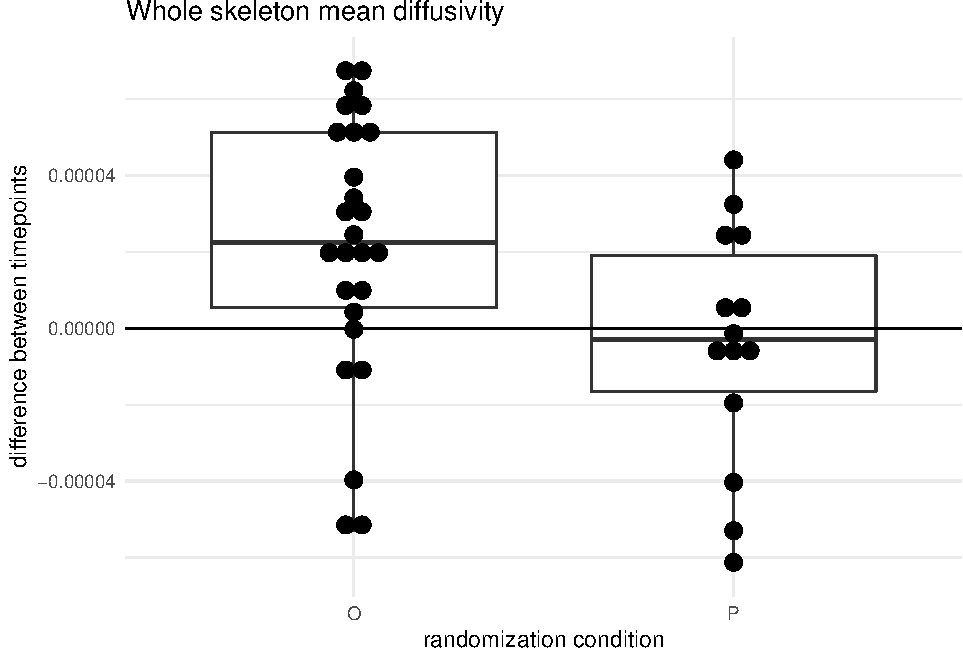
\includegraphics{09_STOPPD_MD-meanFAskel_files/figure-latex/RCT_MD_meanSkel_plot-1.pdf}

\begin{Shaded}
\begin{Highlighting}[]
\NormalTok{fit_rct <-}\StringTok{ }\KeywordTok{lm}\NormalTok{(diffAverageSkel_MD }\OperatorTok{~}\StringTok{ }\NormalTok{randomization, }\DataTypeTok{data=}\NormalTok{ RCT_MD)}
\KeywordTok{print}\NormalTok{(fit_rct)}
\end{Highlighting}
\end{Shaded}

\begin{verbatim}
## 
## Call:
## lm(formula = diffAverageSkel_MD ~ randomization, data = RCT_MD)
## 
## Coefficients:
##    (Intercept)  randomizationP  
##     0.00002180     -0.00002586
\end{verbatim}

\begin{Shaded}
\begin{Highlighting}[]
\KeywordTok{summary}\NormalTok{(fit_rct)}
\end{Highlighting}
\end{Shaded}

\begin{verbatim}
## 
## Call:
## lm(formula = diffAverageSkel_MD ~ randomization, data = RCT_MD)
## 
## Residuals:
##          Min           1Q       Median           3Q          Max 
## -0.000074955 -0.000016010  0.000001087  0.000028189  0.000048102 
## 
## Coefficients:
##                    Estimate   Std. Error t value Pr(>|t|)   
## (Intercept)     0.000021795  0.000006535   3.335  0.00191 **
## randomizationP -0.000025858  0.000011047  -2.341  0.02459 * 
## ---
## Signif. codes:  0 '***' 0.001 '**' 0.01 '*' 0.05 '.' 0.1 ' ' 1
## 
## Residual standard error: 0.00003332 on 38 degrees of freedom
## Multiple R-squared:  0.126,  Adjusted R-squared:  0.103 
## F-statistic: 5.479 on 1 and 38 DF,  p-value: 0.02459
\end{verbatim}

\begin{Shaded}
\begin{Highlighting}[]
\CommentTok{#run linear model with covariates of sex and age}
\NormalTok{fit_rct <-}\StringTok{ }\KeywordTok{lm}\NormalTok{(diffAverageSkel_MD }\OperatorTok{~}\StringTok{ }\NormalTok{randomization }\OperatorTok{+}\StringTok{ }\NormalTok{sex }\OperatorTok{+}\StringTok{ }\NormalTok{age, }\DataTypeTok{data=}\NormalTok{ RCT_MD)}
\KeywordTok{print}\NormalTok{(fit_rct)}
\end{Highlighting}
\end{Shaded}

\begin{verbatim}
## 
## Call:
## lm(formula = diffAverageSkel_MD ~ randomization + sex + age, 
##     data = RCT_MD)
## 
## Coefficients:
##    (Intercept)  randomizationP            sexM             age  
##  0.00001593673  -0.00002622481   0.00000257258   0.00000008944
\end{verbatim}

\begin{Shaded}
\begin{Highlighting}[]
\KeywordTok{summary}\NormalTok{(fit_rct)}
\end{Highlighting}
\end{Shaded}

\begin{verbatim}
## 
## Call:
## lm(formula = diffAverageSkel_MD ~ randomization + sex + age, 
##     data = RCT_MD)
## 
## Residuals:
##          Min           1Q       Median           3Q          Max 
## -0.000078824 -0.000015346  0.000001442  0.000027004  0.000051108 
## 
## Coefficients:
##                      Estimate     Std. Error t value Pr(>|t|)  
## (Intercept)     0.00001593673  0.00002145081   0.743   0.4623  
## randomizationP -0.00002622481  0.00001152451  -2.276   0.0289 *
## sexM            0.00000257258  0.00001109389   0.232   0.8179  
## age             0.00000008944  0.00000039787   0.225   0.8234  
## ---
## Signif. codes:  0 '***' 0.001 '**' 0.01 '*' 0.05 '.' 0.1 ' ' 1
## 
## Residual standard error: 0.00003417 on 36 degrees of freedom
## Multiple R-squared:  0.1292, Adjusted R-squared:  0.05661 
## F-statistic:  1.78 on 3 and 36 DF,  p-value: 0.1684
\end{verbatim}

\begin{Shaded}
\begin{Highlighting}[]
\CommentTok{#run linear model with covariates of sex, age and site}
\NormalTok{fit_rct <-}\StringTok{ }\KeywordTok{lm}\NormalTok{(diffAverageSkel_MD }\OperatorTok{~}\StringTok{ }\NormalTok{randomization }\OperatorTok{+}\StringTok{ }\NormalTok{sex }\OperatorTok{+}\StringTok{ }\NormalTok{age }\OperatorTok{+}\StringTok{ }\NormalTok{site, }\DataTypeTok{data=}\NormalTok{ RCT_MD)}
\KeywordTok{print}\NormalTok{(fit_rct)}
\end{Highlighting}
\end{Shaded}

\begin{verbatim}
## 
## Call:
## lm(formula = diffAverageSkel_MD ~ randomization + sex + age + 
##     site, data = RCT_MD)
## 
## Coefficients:
##    (Intercept)  randomizationP            sexM             age  
##   0.0000015270   -0.0000284379    0.0000026363    0.0000003261  
##        siteMAS         siteNKI         sitePMC  
##   0.0000081404    0.0000119016   -0.0000128742
\end{verbatim}

\begin{Shaded}
\begin{Highlighting}[]
\KeywordTok{summary}\NormalTok{(fit_rct)}
\end{Highlighting}
\end{Shaded}

\begin{verbatim}
## 
## Call:
## lm(formula = diffAverageSkel_MD ~ randomization + sex + age + 
##     site, data = RCT_MD)
## 
## Residuals:
##          Min           1Q       Median           3Q          Max 
## -0.000072064 -0.000010679  0.000000839  0.000020198  0.000049068 
## 
## Coefficients:
##                     Estimate    Std. Error t value Pr(>|t|)  
## (Intercept)     0.0000015270  0.0000244528   0.062   0.9506  
## randomizationP -0.0000284379  0.0000119565  -2.378   0.0233 *
## sexM            0.0000026363  0.0000114702   0.230   0.8196  
## age             0.0000003261  0.0000004465   0.730   0.4703  
## siteMAS         0.0000081404  0.0000152481   0.534   0.5970  
## siteNKI         0.0000119016  0.0000145722   0.817   0.4199  
## sitePMC        -0.0000128742  0.0000179022  -0.719   0.4771  
## ---
## Signif. codes:  0 '***' 0.001 '**' 0.01 '*' 0.05 '.' 0.1 ' ' 1
## 
## Residual standard error: 0.00003478 on 33 degrees of freedom
## Multiple R-squared:  0.1733, Adjusted R-squared:  0.02303 
## F-statistic: 1.153 on 6 and 33 DF,  p-value: 0.3545
\end{verbatim}

\subsection{RCT \& Relapse (with time as
factor)}\label{rct-relapse-with-time-as-factor-3}

\begin{Shaded}
\begin{Highlighting}[]
\NormalTok{RCTRelapse_wholeskelMD <-}\StringTok{ }\NormalTok{RCTRelapse_MD }\OperatorTok
\StringTok{  }\KeywordTok{filter}\NormalTok{(Tract }\OperatorTok{==}\StringTok{ "AverageFA"}\NormalTok{)}
\CommentTok{#plot}
\NormalTok{RCTRelapse_wholeskelMD }\OperatorTok
\StringTok{  }\KeywordTok{ggplot}\NormalTok{(}\KeywordTok{aes}\NormalTok{(}\DataTypeTok{x=}\NormalTok{model_days, }\DataTypeTok{y=}\NormalTok{MD, }\DataTypeTok{colour=}\NormalTok{randomization)) }\OperatorTok{+}\StringTok{ }
\StringTok{  }\KeywordTok{geom_point}\NormalTok{() }\OperatorTok{+}\StringTok{ }
\StringTok{  }\KeywordTok{geom_line}\NormalTok{(}\KeywordTok{aes}\NormalTok{(}\DataTypeTok{group=}\NormalTok{STUDYID), }\DataTypeTok{alpha =} \FloatTok{0.5}\NormalTok{) }\OperatorTok{+}\StringTok{ }
\StringTok{  }\KeywordTok{geom_smooth}\NormalTok{(}\DataTypeTok{method=}\StringTok{"lm"}\NormalTok{, }\DataTypeTok{formula=}\NormalTok{y}\OperatorTok{~}\KeywordTok{poly}\NormalTok{(x,}\DecValTok{1}\NormalTok{)) }\OperatorTok{+}
\StringTok{  }\KeywordTok{ggtitle}\NormalTok{(}\StringTok{"Whole skeleton mean diffusivity over time"}\NormalTok{) }\OperatorTok{+}\StringTok{    }
\StringTok{  }\KeywordTok{xlab}\NormalTok{(}\StringTok{"days between MRIs"}\NormalTok{) }\OperatorTok{+}\StringTok{  }
\StringTok{  }\KeywordTok{ylab}\NormalTok{(}\StringTok{"Mean Diffusivity"}\NormalTok{) }\OperatorTok{+}
\StringTok{  }\KeywordTok{theme_minimal}\NormalTok{()}
\end{Highlighting}
\end{Shaded}

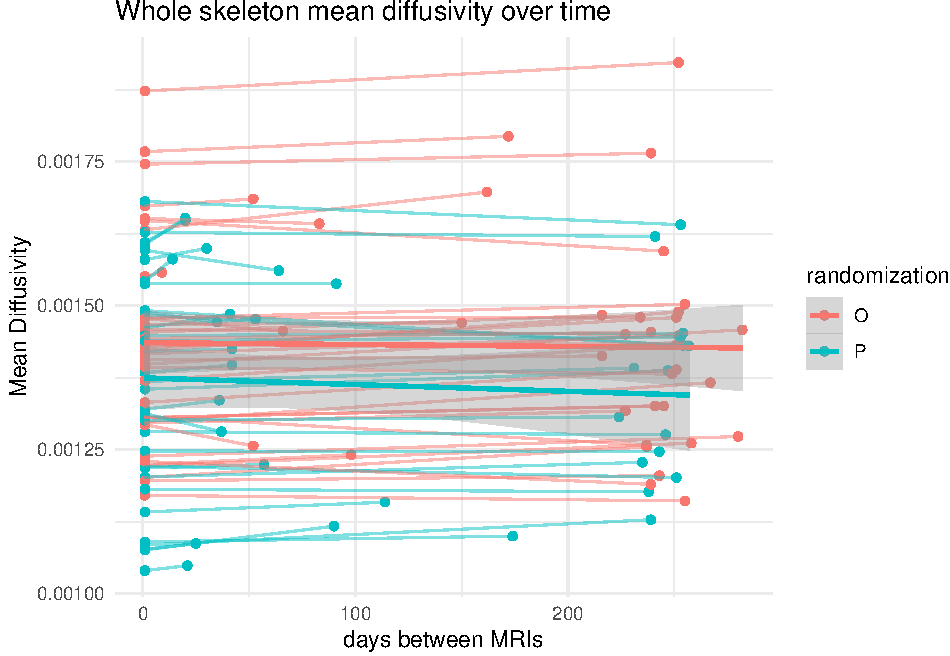
\includegraphics{09_STOPPD_MD-meanFAskel_files/figure-latex/RCTRelapse_MD_plot-1.pdf}

\begin{Shaded}
\begin{Highlighting}[]
\CommentTok{#run mixed linear model, with covariates}
\NormalTok{fit_all <-}\StringTok{ }\KeywordTok{lmer}\NormalTok{(MD }\OperatorTok{~}\StringTok{ }\NormalTok{randomization}\OperatorTok{*}\NormalTok{model_days }\OperatorTok{+}\StringTok{ }\NormalTok{sex }\OperatorTok{+}\StringTok{ }\NormalTok{age }\OperatorTok{+}\StringTok{ }\NormalTok{(}\DecValTok{1}\OperatorTok{|}\NormalTok{STUDYID), }\DataTypeTok{data=}\NormalTok{ RCTRelapse_wholeskelMD)}
\KeywordTok{summary}\NormalTok{(fit_all)}
\end{Highlighting}
\end{Shaded}

\begin{verbatim}
## Linear mixed model fit by REML. t-tests use Satterthwaite's method [
## lmerModLmerTest]
## Formula: MD ~ randomization * model_days + sex + age + (1 | STUDYID)
##    Data: RCTRelapse_wholeskelMD
## 
## REML criterion at convergence: -2207.3
## 
## Scaled residuals: 
##      Min       1Q   Median       3Q      Max 
## -1.80780 -0.44415 -0.02353  0.38354  1.76631 
## 
## Random effects:
##  Groups   Name        Variance        Std.Dev.  
##  STUDYID  (Intercept) 0.0000000160882 0.00012684
##  Residual             0.0000000004334 0.00002082
## Number of obs: 142, groups:  STUDYID, 71
## 
## Fixed effects:
##                                 Estimate     Std. Error             df
## (Intercept)                0.00096997852  0.00005883295 67.24042295176
## randomizationP            -0.00006889045  0.00003058032 68.37097299833
## model_days                 0.00000008709  0.00000002198 69.19446523698
## sexM                       0.00003079208  0.00003052508 66.99217346591
## age                        0.00000802914  0.00000099148 66.99260766274
## randomizationP:model_days -0.00000009395  0.00000003705 69.48340161813
##                           t value             Pr(>|t|)    
## (Intercept)                16.487 < 0.0000000000000002 ***
## randomizationP             -2.253             0.027486 *  
## model_days                  3.963             0.000178 ***
## sexM                        1.009             0.316726    
## age                         8.098       0.000000000016 ***
## randomizationP:model_days  -2.536             0.013471 *  
## ---
## Signif. codes:  0 '***' 0.001 '**' 0.01 '*' 0.05 '.' 0.1 ' ' 1
## 
## Correlation of Fixed Effects:
##             (Intr) rndmzP mdl_dy sexM   age   
## randomiztnP -0.205                            
## model_days  -0.043  0.075                     
## sexM        -0.174  0.050  0.002              
## age         -0.899 -0.061  0.004 -0.085       
## rndmztnP:m_  0.024 -0.099 -0.593  0.002 -0.001
\end{verbatim}

\subsection{just wanna through in one site
model..}\label{just-wanna-through-in-one-site-model..-1}

\begin{Shaded}
\begin{Highlighting}[]
\CommentTok{#run mixed linear model, with covariates}
\NormalTok{fit_all <-}\StringTok{ }\KeywordTok{lmer}\NormalTok{(MD }\OperatorTok{~}\StringTok{ }\NormalTok{randomization}\OperatorTok{*}\NormalTok{model_days }\OperatorTok{+}\StringTok{ }\NormalTok{sex }\OperatorTok{+}\StringTok{ }\NormalTok{age }\OperatorTok{+}\StringTok{ }\NormalTok{site }\OperatorTok{+}\StringTok{ }\NormalTok{(}\DecValTok{1}\OperatorTok{|}\NormalTok{STUDYID), }\DataTypeTok{data=}\NormalTok{ RCTRelapse_wholeskelMD)}
\KeywordTok{summary}\NormalTok{(fit_all)}
\end{Highlighting}
\end{Shaded}

\begin{verbatim}
## Linear mixed model fit by REML. t-tests use Satterthwaite's method [
## lmerModLmerTest]
## Formula: 
## MD ~ randomization * model_days + sex + age + site + (1 | STUDYID)
##    Data: RCTRelapse_wholeskelMD
## 
## REML criterion at convergence: -2201.2
## 
## Scaled residuals: 
##      Min       1Q   Median       3Q      Max 
## -1.76367 -0.44166 -0.00876  0.39208  1.91515 
## 
## Random effects:
##  Groups   Name        Variance        Std.Dev.  
##  STUDYID  (Intercept) 0.0000000077233 0.00008788
##  Residual             0.0000000004336 0.00002082
## Number of obs: 142, groups:  STUDYID, 71
## 
## Fixed effects:
##                                 Estimate     Std. Error             df
## (Intercept)                0.00107616983  0.00004312397 64.39556122315
## randomizationP            -0.00003551473  0.00002183608 66.56430055822
## model_days                 0.00000008624  0.00000002197 69.34666962025
## sexM                       0.00005950979  0.00002160794 63.94765683051
## age                        0.00000761020  0.00000069842 63.95027065884
## siteMAS                   -0.00019539464  0.00002789578 63.94948973534
## siteNKI                   -0.00018424524  0.00003016377 63.95445709082
## sitePMC                   -0.00018719886  0.00003103365 63.94534349730
## randomizationP:model_days -0.00000009587  0.00000003699 69.94739066144
##                           t value             Pr(>|t|)    
## (Intercept)                24.955 < 0.0000000000000002 ***
## randomizationP             -1.626             0.108585    
## model_days                  3.926             0.000201 ***
## sexM                        2.754             0.007655 ** 
## age                        10.896 0.000000000000000325 ***
## siteMAS                    -7.004 0.000000001833884447 ***
## siteNKI                    -6.108 0.000000066268061845 ***
## sitePMC                    -6.032 0.000000089508213317 ***
## randomizationP:model_days  -2.592             0.011617 *  
## ---
## Signif. codes:  0 '***' 0.001 '**' 0.01 '*' 0.05 '.' 0.1 ' ' 1
## 
## Correlation of Fixed Effects:
##             (Intr) rndmzP mdl_dy sexM   age    sitMAS sitNKI sitPMC
## randomiztnP -0.137                                                 
## model_days  -0.059  0.105                                          
## sexM        -0.126  0.072  0.003                                   
## age         -0.879 -0.077  0.006 -0.086                            
## siteMAS     -0.290 -0.174  0.004 -0.092  0.124                     
## siteNKI     -0.175 -0.122 -0.008 -0.122  0.013  0.355              
## sitePMC     -0.153 -0.092  0.000 -0.146 -0.007  0.341  0.320       
## rndmztnP:m_  0.032 -0.139 -0.594  0.001 -0.002  0.001  0.007  0.002
\end{verbatim}

\begin{Shaded}
\begin{Highlighting}[]
\NormalTok{#cleanup}
\NormalTok{rm('df', 'fit_all', 'fit_rct', 'MD', 'plot', 'RCT_FA', 'RCTRelapse_FA')}
\end{Highlighting}
\end{Shaded}

\section{Freesurfer Derived Subcortical
Volumes}\label{freesurfer-derived-subcortical-volumes}

\begin{Shaded}
\begin{Highlighting}[]
\KeywordTok{library}\NormalTok{(tidyverse)}
\end{Highlighting}
\end{Shaded}

\begin{verbatim}
## -- Attaching packages --------------------------------------------------------------------------------------------- tidyverse 1.2.1 --
\end{verbatim}

\begin{verbatim}
## √ ggplot2 3.1.0     √ purrr   0.2.4
## √ tibble  1.4.1     √ dplyr   0.7.7
## √ tidyr   0.7.2     √ stringr 1.2.0
## √ readr   1.1.1     √ forcats 0.2.0
\end{verbatim}

\begin{verbatim}
## -- Conflicts ------------------------------------------------------------------------------------------------ tidyverse_conflicts() --
## x dplyr::filter() masks stats::filter()
## x dplyr::lag()    masks stats::lag()
\end{verbatim}

\begin{Shaded}
\begin{Highlighting}[]
\KeywordTok{library}\NormalTok{(lme4)}
\end{Highlighting}
\end{Shaded}

\begin{verbatim}
## Loading required package: Matrix
\end{verbatim}

\begin{verbatim}
## 
## Attaching package: 'Matrix'
\end{verbatim}

\begin{verbatim}
## The following object is masked from 'package:tidyr':
## 
##     expand
\end{verbatim}

\begin{verbatim}
## Loading required package: methods
\end{verbatim}

\begin{Shaded}
\begin{Highlighting}[]
\KeywordTok{library}\NormalTok{(lmerTest)}
\end{Highlighting}
\end{Shaded}

\begin{verbatim}
## 
## Attaching package: 'lmerTest'
\end{verbatim}

\begin{verbatim}
## The following object is masked from 'package:lme4':
## 
##     lmer
\end{verbatim}

\begin{verbatim}
## The following object is masked from 'package:stats':
## 
##     step
\end{verbatim}

\begin{Shaded}
\begin{Highlighting}[]
\NormalTok{df <-}\StringTok{ }\KeywordTok{read_csv}\NormalTok{(}\StringTok{"../generated_csvs/STOPPD_masterDF_2018-11-05.csv"}\NormalTok{,}\DataTypeTok{na =} \StringTok{"empty"}\NormalTok{) }\CommentTok{#spreadsheet created by 03_STOPPD_masterDF.rmd}
\end{Highlighting}
\end{Shaded}

\begin{verbatim}
## Parsed with column specification:
## cols(
##   .default = col_character(),
##   STUDYID = col_integer()
## )
\end{verbatim}

\begin{verbatim}
## See spec(...) for full column specifications.
\end{verbatim}

\begin{Shaded}
\begin{Highlighting}[]
\NormalTok{FS <-}\StringTok{ }\KeywordTok{read_csv}\NormalTok{(}\StringTok{'../data/fs-enigma-long_201811/LandRvolumes.csv'}\NormalTok{) }\CommentTok{#bring in subcortical data, from pipelines}
\end{Highlighting}
\end{Shaded}

\begin{verbatim}
## Parsed with column specification:
## cols(
##   SubjID = col_character(),
##   LLatVent = col_double(),
##   RLatVent = col_double(),
##   Lthal = col_double(),
##   Rthal = col_double(),
##   Lcaud = col_double(),
##   Rcaud = col_double(),
##   Lput = col_double(),
##   Rput = col_double(),
##   Lpal = col_double(),
##   Rpal = col_double(),
##   Lhippo = col_double(),
##   Rhippo = col_double(),
##   Lamyg = col_double(),
##   Ramyg = col_double(),
##   Laccumb = col_double(),
##   Raccumb = col_double(),
##   ICV = col_double()
## )
\end{verbatim}

\begin{Shaded}
\begin{Highlighting}[]
\CommentTok{# remove participants that did not complete first and second scan (n=74)}
\CommentTok{# then add offlabel and dateDiff (in days columns)}
\CommentTok{# + a scan is by definition offlabel if it is the third scan}
\CommentTok{# then select the cols for analysis}
\NormalTok{df <-}\StringTok{ }\NormalTok{df }\OperatorTok
\StringTok{  }\KeywordTok{filter}\NormalTok{(first_complete }\OperatorTok{==}\StringTok{ "Yes"}\NormalTok{, }
\NormalTok{         second_complete }\OperatorTok{==}\StringTok{ "Yes"}\NormalTok{,}
\NormalTok{         MR_exclusion }\OperatorTok{==}\StringTok{ "No"}\NormalTok{) }\OperatorTok
\StringTok{  }\KeywordTok{mutate}\NormalTok{(}\DataTypeTok{offLabel  =} \KeywordTok{if_else}\NormalTok{(third_complete }\OperatorTok{==}\StringTok{ "Yes"}\NormalTok{, }\StringTok{"Yes"}\NormalTok{, }\StringTok{''}\NormalTok{),}
         \DataTypeTok{dateDiff =} \KeywordTok{round}\NormalTok{(}\KeywordTok{difftime}\NormalTok{(second_date, first_date, }\DataTypeTok{units =} \StringTok{"days"}\NormalTok{), }\DecValTok{0}\NormalTok{),}
         \DataTypeTok{STUDYID =} \KeywordTok{parse_character}\NormalTok{(STUDYID),}
         \DataTypeTok{age =} \KeywordTok{parse_number}\NormalTok{(age)) }\OperatorTok
\StringTok{  }\KeywordTok{rename}\NormalTok{(}\DataTypeTok{category =} \StringTok{"second_timepoint"}\NormalTok{) }\OperatorTok
\StringTok{  }\KeywordTok{select}\NormalTok{(STUDYID, randomization, sex, age, category, offLabel, dateDiff)}
\end{Highlighting}
\end{Shaded}

\subsection{cleaning the CT data}\label{cleaning-the-ct-data-1}

\begin{Shaded}
\begin{Highlighting}[]
\CommentTok{# separating the subject id and anything afterwards to identify the longtudinal pipeline participants}
\CommentTok{# separating the subject id into site, "STUDYID" and timepoint columns}
\CommentTok{# filtering (two steps) to only include the longitudinal pipeline data}
\NormalTok{FS_long <-}\StringTok{ }\NormalTok{FS }\OperatorTok
\StringTok{  }\KeywordTok{separate}\NormalTok{(SubjID, }\DataTypeTok{into =} \KeywordTok{c}\NormalTok{(}\StringTok{"subid"}\NormalTok{, }\StringTok{"longitudinal_pipe"}\NormalTok{), }\DataTypeTok{sep =} \StringTok{'}\CharTok{\textbackslash{}\textbackslash{}}\StringTok{.'}\NormalTok{, }\DataTypeTok{extra =} \StringTok{"drop"}\NormalTok{, }\DataTypeTok{fill =} \StringTok{"right"}\NormalTok{) }\OperatorTok
\StringTok{  }\KeywordTok{separate}\NormalTok{(subid, }\DataTypeTok{into =} \KeywordTok{c}\NormalTok{(}\StringTok{"study"}\NormalTok{, }\StringTok{"site"}\NormalTok{, }\StringTok{"STUDYID"}\NormalTok{, }\StringTok{"timepoint"}\NormalTok{), }\DataTypeTok{fill =} \StringTok{"right"}\NormalTok{) }\OperatorTok
\StringTok{  }\KeywordTok{filter}\NormalTok{(longitudinal_pipe }\OperatorTok{==}\StringTok{ "long"}\NormalTok{) }\OperatorTok
\StringTok{  }\KeywordTok{filter}\NormalTok{(timepoint }\OperatorTok{!=}\StringTok{ "00"}\NormalTok{, timepoint }\OperatorTok{!=}\StringTok{ "03"}\NormalTok{, timepoint }\OperatorTok{!=}\StringTok{ ""}\NormalTok{)}

\CommentTok{# adding columns that combine L and R}
\NormalTok{FS_long_plus <-}\StringTok{ }\NormalTok{FS_long }\OperatorTok
\StringTok{  }\KeywordTok{mutate}\NormalTok{(}\DataTypeTok{Thalamus =}\NormalTok{ Lthal }\OperatorTok{+}\StringTok{ }\NormalTok{Rthal,}
         \DataTypeTok{Hippocampus =}\NormalTok{ Lhippo }\OperatorTok{+}\StringTok{ }\NormalTok{Rhippo,}
         \DataTypeTok{Striatum =}\NormalTok{ Lcaud }\OperatorTok{+}\StringTok{ }\NormalTok{Rcaud }\OperatorTok{+}\StringTok{ }\NormalTok{Lput }\OperatorTok{+}\StringTok{ }\NormalTok{Rput)}


\CommentTok{# move CT from long to wide format}
\NormalTok{FS_wide <-}\StringTok{ }\NormalTok{FS_long_plus }\OperatorTok
\StringTok{  }\KeywordTok{gather}\NormalTok{(region, volume, }\OperatorTok{-}\NormalTok{study, }\OperatorTok{-}\NormalTok{site, }\OperatorTok{-}\NormalTok{timepoint, }\OperatorTok{-}\NormalTok{STUDYID, }\OperatorTok{-}\NormalTok{longitudinal_pipe) }\OperatorTok
\StringTok{  }\KeywordTok{spread}\NormalTok{(timepoint, volume) }\OperatorTok
\StringTok{  }\KeywordTok{mutate}\NormalTok{(}\DataTypeTok{change =} \StringTok{`}\DataTypeTok{02}\StringTok{`} \OperatorTok{-}\StringTok{ `}\DataTypeTok{01}\StringTok{`}\NormalTok{) }\OperatorTok
\StringTok{  }\KeywordTok{gather}\NormalTok{(timepoint, volume, }\StringTok{`}\DataTypeTok{01}\StringTok{`}\NormalTok{, }\StringTok{`}\DataTypeTok{02}\StringTok{`}\NormalTok{, change) }\OperatorTok
\StringTok{  }\KeywordTok{unite}\NormalTok{(newcolnames, region, timepoint) }\OperatorTok
\StringTok{  }\KeywordTok{spread}\NormalTok{(newcolnames, volume)}
\end{Highlighting}
\end{Shaded}

\begin{Shaded}
\begin{Highlighting}[]
\CommentTok{# merge CT values with df}
\NormalTok{ana_df <-}\StringTok{ }\KeywordTok{inner_join}\NormalTok{(df, FS_wide, }\DataTypeTok{by=}\StringTok{'STUDYID'}\NormalTok{) }\OperatorTok
\StringTok{    }\KeywordTok{mutate}\NormalTok{(}\DataTypeTok{STUDYID =} \KeywordTok{as.character}\NormalTok{(STUDYID),}
         \DataTypeTok{dateDiff =} \KeywordTok{as.numeric}\NormalTok{(dateDiff),}
         \DataTypeTok{RandomArm =} \KeywordTok{factor}\NormalTok{(randomization, }
                       \DataTypeTok{levels =} \KeywordTok{c}\NormalTok{(}\StringTok{"O"}\NormalTok{, }\StringTok{"P"}\NormalTok{),}
                       \DataTypeTok{labels =} \KeywordTok{c}\NormalTok{(}\StringTok{"Olanzapine"}\NormalTok{, }\StringTok{"Placebo"}\NormalTok{))) }

\CommentTok{# write.csv}
\KeywordTok{write_csv}\NormalTok{(ana_df, }\StringTok{'../generated_csvs/STOPPD_participants_LandRVolumes_20181116.csv'}\NormalTok{)}
\end{Highlighting}
\end{Shaded}

\subsection{report any mising values from clinical trial
sample}\label{report-any-mising-values-from-clinical-trial-sample-1}

\begin{Shaded}
\begin{Highlighting}[]
\KeywordTok{anti_join}\NormalTok{(df, FS_wide, }\DataTypeTok{by=}\StringTok{'STUDYID'}\NormalTok{) }\OperatorTok
\StringTok{  }\KeywordTok{summarise}\NormalTok{(}\StringTok{`}\DataTypeTok{Number of participants missing}\StringTok{`}\NormalTok{ =}\StringTok{ }\KeywordTok{n}\NormalTok{()) }\OperatorTok
\StringTok{  }\NormalTok{knitr}\OperatorTok{::}\KeywordTok{kable}\NormalTok{()}
\end{Highlighting}
\end{Shaded}

\begin{tabular}{r}
\hline
Number of participants missing\\
\hline
0\\
\hline
\end{tabular}

\begin{Shaded}
\begin{Highlighting}[]
\NormalTok{ana_df }\OperatorTok
\StringTok{  }\KeywordTok{filter}\NormalTok{(}\KeywordTok{is.na}\NormalTok{(ICV_}\DecValTok{01}\NormalTok{)) }\OperatorTok
\StringTok{  }\KeywordTok{summarise}\NormalTok{(}\StringTok{`}\DataTypeTok{Number of participants missing timepoint 01}\StringTok{`}\NormalTok{ =}\StringTok{ }\KeywordTok{n}\NormalTok{()) }\OperatorTok
\StringTok{  }\NormalTok{knitr}\OperatorTok{::}\KeywordTok{kable}\NormalTok{()}
\end{Highlighting}
\end{Shaded}

\begin{tabular}{r}
\hline
Number of participants missing timepoint 01\\
\hline
0\\
\hline
\end{tabular}

\begin{Shaded}
\begin{Highlighting}[]
\NormalTok{ana_df }\OperatorTok
\StringTok{  }\KeywordTok{filter}\NormalTok{(}\KeywordTok{is.na}\NormalTok{(ICV_}\DecValTok{02}\NormalTok{)) }\OperatorTok
\StringTok{  }\KeywordTok{summarise}\NormalTok{(}\StringTok{`}\DataTypeTok{Number of participants missing timepoint 02}\StringTok{`}\NormalTok{ =}\StringTok{ }\KeywordTok{n}\NormalTok{()) }\OperatorTok
\StringTok{  }\NormalTok{knitr}\OperatorTok{::}\KeywordTok{kable}\NormalTok{()}
\end{Highlighting}
\end{Shaded}

\begin{tabular}{r}
\hline
Number of participants missing timepoint 02\\
\hline
0\\
\hline
\end{tabular}

\subsection{creating an control error term calculating data
frame}\label{creating-an-control-error-term-calculating-data-frame}

\begin{Shaded}
\begin{Highlighting}[]
\NormalTok{## identify the repeat control in a column and mangle the STUDYID to match in a new column}
\NormalTok{FS_long1 <-}\StringTok{ }\NormalTok{FS_long_plus }\OperatorTok
\StringTok{  }\KeywordTok{mutate}\NormalTok{(}\DataTypeTok{repeat_run =} \KeywordTok{if_else}\NormalTok{(}\KeywordTok{str_sub}\NormalTok{(STUDYID,}\DecValTok{1}\NormalTok{,}\DecValTok{1}\NormalTok{)}\OperatorTok{==}\StringTok{"R"}\NormalTok{, }\StringTok{"02"}\NormalTok{, }\StringTok{"01"}\NormalTok{),}
         \DataTypeTok{STUDYID =} \KeywordTok{str_replace}\NormalTok{(STUDYID, }\StringTok{'R'}\NormalTok{,}\StringTok{""}\NormalTok{)) }

\NormalTok{## extra the repeat study ids as a character vector}
\NormalTok{repeat_ids <-}\StringTok{ }\KeywordTok{filter}\NormalTok{(FS_long1, repeat_run }\OperatorTok{==}\StringTok{ "02"}\NormalTok{)}\OperatorTok{$}\NormalTok{STUDYID}

\NormalTok{## filter for only the subjects who are in the repeats list then switch to wide format}
\NormalTok{FS_wide_controls <-}\StringTok{ }\NormalTok{FS_long1 }\OperatorTok
\StringTok{  }\KeywordTok{filter}\NormalTok{(STUDYID }\OperatorTok\StringTok{ }\NormalTok{repeat_ids) }\OperatorTok\StringTok{ }
\StringTok{  }\KeywordTok{gather}\NormalTok{(region, volume, }\OperatorTok{-}\NormalTok{study, }\OperatorTok{-}\NormalTok{site, }\OperatorTok{-}\NormalTok{timepoint, }\OperatorTok{-}\NormalTok{STUDYID, }\OperatorTok{-}\NormalTok{longitudinal_pipe, }\OperatorTok{-}\NormalTok{repeat_run) }\OperatorTok
\StringTok{  }\KeywordTok{unite}\NormalTok{(newcolnames, region, repeat_run) }\OperatorTok
\StringTok{  }\KeywordTok{spread}\NormalTok{(newcolnames, volume)}

\CommentTok{#write.csv}
  \KeywordTok{write.csv}\NormalTok{(FS_wide_controls, }\StringTok{'../generated_csvs/STOPPD_errorControls_LandRVolumes_2018-11-05.csv'}\NormalTok{, }\DataTypeTok{row.names =} \OtherTok{FALSE}\NormalTok{)}
  
\KeywordTok{rm}\NormalTok{(FS_long1, repeat_ids)}
\end{Highlighting}
\end{Shaded}

\subsection{run RCT analysis (because it's simpler across
volumes)}\label{run-rct-analysis-because-its-simpler-across-volumes}

\begin{Shaded}
\begin{Highlighting}[]
\CommentTok{# make sure that STUDYID is an character not a number}
\CommentTok{# make sure that dateDiff is a number, not an interger}
\CommentTok{# label the randomization variable  }
\NormalTok{RCT_SubCort <-}\StringTok{ }\NormalTok{ana_df }\OperatorTok

\StringTok{  }\KeywordTok{filter}\NormalTok{(category }\OperatorTok{==}\StringTok{ "RCT"}\NormalTok{)}
\end{Highlighting}
\end{Shaded}

\begin{Shaded}
\begin{Highlighting}[]
\CommentTok{#boxplot of difference in thickness (y axis) by randomization group (x axis)}
\NormalTok{RCT_SubCort  }\OperatorTok
\StringTok{  }\KeywordTok{gather}\NormalTok{(region, volume_change, Thalamus_change, Hippocampus_change, Striatum_change) }\OperatorTok
\StringTok{  }\KeywordTok{mutate}\NormalTok{(}\DataTypeTok{Region =} \KeywordTok{str_replace}\NormalTok{(region, }\StringTok{'_change'}\NormalTok{,}\StringTok{''}\NormalTok{)) }\OperatorTok
\KeywordTok{ggplot}\NormalTok{(}\KeywordTok{aes}\NormalTok{(}\DataTypeTok{x=}\NormalTok{ RandomArm, }\DataTypeTok{y =}\NormalTok{ volume_change)) }\OperatorTok{+}\StringTok{ }
\StringTok{     }\KeywordTok{geom_boxplot}\NormalTok{(}\DataTypeTok{outlier.shape =} \OtherTok{NA}\NormalTok{) }\OperatorTok{+}\StringTok{ }
\StringTok{     }\KeywordTok{geom_dotplot}\NormalTok{(}\DataTypeTok{binaxis =} \StringTok{'y'}\NormalTok{, }\DataTypeTok{stackdir =} \StringTok{'center'}\NormalTok{) }\OperatorTok{+}
\StringTok{     }\KeywordTok{geom_hline}\NormalTok{(}\DataTypeTok{yintercept =} \DecValTok{0}\NormalTok{) }\OperatorTok{+}
\StringTok{     }\KeywordTok{ggtitle}\NormalTok{(}\StringTok{"Freesurfer Subcortical Volume Changes"}\NormalTok{) }\OperatorTok{+}
\StringTok{     }\KeywordTok{xlab}\NormalTok{(}\OtherTok{NULL}\NormalTok{) }\OperatorTok{+}
\StringTok{     }\KeywordTok{ylab}\NormalTok{(}\StringTok{"Change in Volume"}\NormalTok{) }\OperatorTok{+}
\StringTok{     }\KeywordTok{facet_wrap}\NormalTok{(}\OperatorTok{~}\NormalTok{Region) }\OperatorTok{+}
\StringTok{     }\KeywordTok{theme_bw}\NormalTok{()}
\end{Highlighting}
\end{Shaded}

\begin{verbatim}
## `stat_bindot()` using `bins = 30`. Pick better value with `binwidth`.
\end{verbatim}

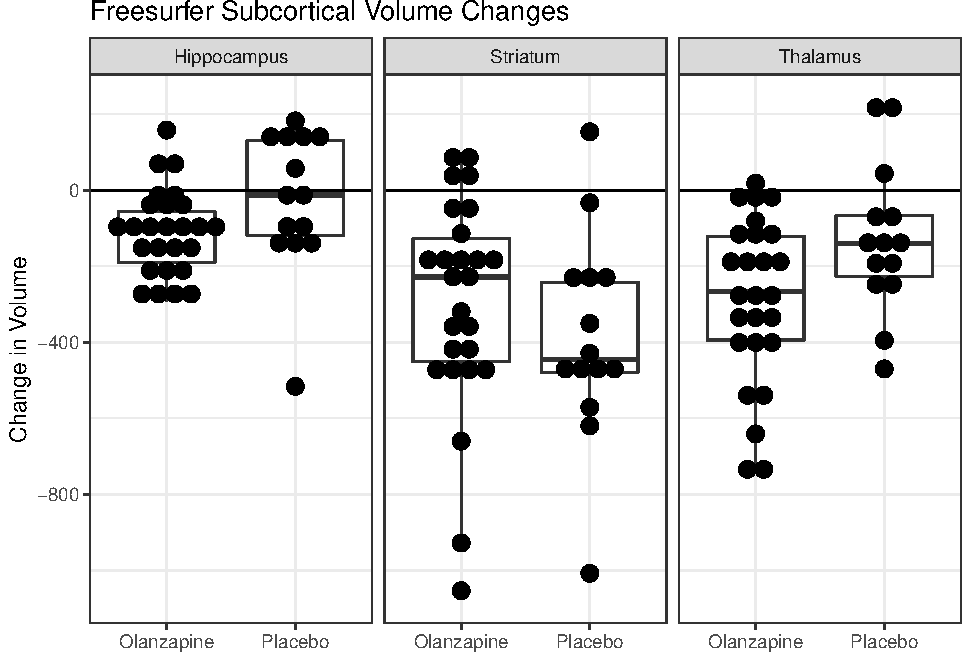
\includegraphics{10_STOPPD_freesurfer_subcortical_files/figure-latex/10-boxplot-ROIs-1.pdf}
\#\#\# Running RCT Linear Models

\paragraph{Thalamus}\label{thalamus}

\begin{Shaded}
\begin{Highlighting}[]
\CommentTok{#run linear model without covariates}
\NormalTok{  fit_rct <-}\StringTok{ }\KeywordTok{lm}\NormalTok{(Thalamus_change }\OperatorTok{~}\StringTok{ }\NormalTok{RandomArm, }\DataTypeTok{data=}\NormalTok{ RCT_SubCort)}
  \KeywordTok{summary}\NormalTok{(fit_rct)}
\end{Highlighting}
\end{Shaded}

\begin{verbatim}
## 
## Call:
## lm(formula = Thalamus_change ~ RandomArm, data = RCT_SubCort)
## 
## Residuals:
##     Min      1Q  Median      3Q     Max 
## -454.67 -105.09    3.09  155.71  366.04 
## 
## Coefficients:
##                  Estimate Std. Error t value Pr(>|t|)    
## (Intercept)       -286.13      41.25  -6.937    3e-08 ***
## RandomArmPlacebo   157.29      69.73   2.256   0.0299 *  
## ---
## Signif. codes:  0 '***' 0.001 '**' 0.01 '*' 0.05 '.' 0.1 ' ' 1
## 
## Residual standard error: 210.3 on 38 degrees of freedom
## Multiple R-squared:  0.1181, Adjusted R-squared:  0.09489 
## F-statistic: 5.089 on 1 and 38 DF,  p-value: 0.02992
\end{verbatim}

\begin{Shaded}
\begin{Highlighting}[]
\CommentTok{#run linear model with covariates of sex and age}
\NormalTok{  fit_rct <-}\StringTok{ }\KeywordTok{lm}\NormalTok{(Thalamus_change }\OperatorTok{~}\StringTok{ }\NormalTok{RandomArm }\OperatorTok{+}\StringTok{ }\NormalTok{sex }\OperatorTok{+}\StringTok{ }\NormalTok{age, }\DataTypeTok{data=}\NormalTok{ RCT_SubCort)}
  \KeywordTok{summary}\NormalTok{(fit_rct)}
\end{Highlighting}
\end{Shaded}

\begin{verbatim}
## 
## Call:
## lm(formula = Thalamus_change ~ RandomArm + sex + age, data = RCT_SubCort)
## 
## Residuals:
##     Min      1Q  Median      3Q     Max 
## -484.06 -102.67   17.14  139.25  326.59 
## 
## Coefficients:
##                  Estimate Std. Error t value Pr(>|t|)  
## (Intercept)      -188.053    134.129  -1.402   0.1695  
## RandomArmPlacebo  169.144     72.061   2.347   0.0245 *
## sexM               30.398     69.369   0.438   0.6639  
## age                -2.146      2.488  -0.863   0.3940  
## ---
## Signif. codes:  0 '***' 0.001 '**' 0.01 '*' 0.05 '.' 0.1 ' ' 1
## 
## Residual standard error: 213.7 on 36 degrees of freedom
## Multiple R-squared:  0.1377, Adjusted R-squared:  0.06582 
## F-statistic: 1.916 on 3 and 36 DF,  p-value: 0.1444
\end{verbatim}

\begin{Shaded}
\begin{Highlighting}[]
\CommentTok{#run linear model with covariates of sex and age}
\NormalTok{  fit_rct <-}\StringTok{ }\KeywordTok{lm}\NormalTok{(Thalamus_change }\OperatorTok{~}\StringTok{ }\NormalTok{RandomArm }\OperatorTok{+}\StringTok{ }\NormalTok{sex }\OperatorTok{+}\StringTok{ }\NormalTok{age }\OperatorTok{+}\StringTok{ }\NormalTok{site, }\DataTypeTok{data=}\NormalTok{ RCT_SubCort)}
  \KeywordTok{summary}\NormalTok{(fit_rct)}
\end{Highlighting}
\end{Shaded}

\begin{verbatim}
## 
## Call:
## lm(formula = Thalamus_change ~ RandomArm + sex + age + site, 
##     data = RCT_SubCort)
## 
## Residuals:
##     Min      1Q  Median      3Q     Max 
## -396.26 -147.24   65.82  121.84  294.44 
## 
## Coefficients:
##                  Estimate Std. Error t value Pr(>|t|)  
## (Intercept)      -302.140    144.384  -2.093   0.0442 *
## RandomArmPlacebo  145.518     70.598   2.061   0.0472 *
## sexM                7.308     67.727   0.108   0.9147  
## age                -1.325      2.636  -0.503   0.6186  
## siteMAS           171.904     90.034   1.909   0.0649 .
## siteNKI           179.824     86.043   2.090   0.0444 *
## sitePMC            90.282    105.706   0.854   0.3992  
## ---
## Signif. codes:  0 '***' 0.001 '**' 0.01 '*' 0.05 '.' 0.1 ' ' 1
## 
## Residual standard error: 205.3 on 33 degrees of freedom
## Multiple R-squared:   0.27,  Adjusted R-squared:  0.1373 
## F-statistic: 2.035 on 6 and 33 DF,  p-value: 0.08872
\end{verbatim}

\paragraph{Striatum}\label{striatum}

\begin{Shaded}
\begin{Highlighting}[]
\CommentTok{#run linear model without covariates}
\NormalTok{  fit_rct <-}\StringTok{ }\KeywordTok{lm}\NormalTok{(Striatum_change }\OperatorTok{~}\StringTok{ }\NormalTok{RandomArm, }\DataTypeTok{data=}\NormalTok{ RCT_SubCort)}
  \KeywordTok{print}\NormalTok{(fit_rct)}
\end{Highlighting}
\end{Shaded}

\begin{verbatim}
## 
## Call:
## lm(formula = Striatum_change ~ RandomArm, data = RCT_SubCort)
## 
## Coefficients:
##      (Intercept)  RandomArmPlacebo  
##          -296.60            -91.83
\end{verbatim}

\begin{Shaded}
\begin{Highlighting}[]
  \KeywordTok{summary}\NormalTok{(fit_rct)}
\end{Highlighting}
\end{Shaded}

\begin{verbatim}
## 
## Call:
## lm(formula = Striatum_change ~ RandomArm, data = RCT_SubCort)
## 
## Residuals:
##     Min      1Q  Median      3Q     Max 
## -756.70 -141.60    8.11  153.80  542.53 
## 
## Coefficients:
##                  Estimate Std. Error t value Pr(>|t|)    
## (Intercept)       -296.60      55.23  -5.370 4.15e-06 ***
## RandomArmPlacebo   -91.83      93.35  -0.984    0.331    
## ---
## Signif. codes:  0 '***' 0.001 '**' 0.01 '*' 0.05 '.' 0.1 ' ' 1
## 
## Residual standard error: 281.6 on 38 degrees of freedom
## Multiple R-squared:  0.02483,    Adjusted R-squared:  -0.0008284 
## F-statistic: 0.9677 on 1 and 38 DF,  p-value: 0.3315
\end{verbatim}

\begin{Shaded}
\begin{Highlighting}[]
\CommentTok{#run linear model with covariates of sex and age}
\NormalTok{  fit_rct <-}\StringTok{ }\KeywordTok{lm}\NormalTok{(Striatum_change }\OperatorTok{~}\StringTok{ }\NormalTok{RandomArm }\OperatorTok{+}\StringTok{ }\NormalTok{sex }\OperatorTok{+}\StringTok{ }\NormalTok{age, }\DataTypeTok{data=}\NormalTok{ RCT_SubCort)}
  \KeywordTok{print}\NormalTok{(fit_rct)}
\end{Highlighting}
\end{Shaded}

\begin{verbatim}
## 
## Call:
## lm(formula = Striatum_change ~ RandomArm + sex + age, data = RCT_SubCort)
## 
## Coefficients:
##      (Intercept)  RandomArmPlacebo              sexM               age  
##         -169.875           -80.518           -12.233            -2.318
\end{verbatim}

\begin{Shaded}
\begin{Highlighting}[]
  \KeywordTok{summary}\NormalTok{(fit_rct)}
\end{Highlighting}
\end{Shaded}

\begin{verbatim}
## 
## Call:
## lm(formula = Striatum_change ~ RandomArm + sex + age, data = RCT_SubCort)
## 
## Residuals:
##     Min      1Q  Median      3Q     Max 
## -772.16 -141.82    9.74  154.93  552.85 
## 
## Coefficients:
##                  Estimate Std. Error t value Pr(>|t|)
## (Intercept)      -169.875    180.214  -0.943    0.352
## RandomArmPlacebo  -80.518     96.821  -0.832    0.411
## sexM              -12.233     93.203  -0.131    0.896
## age                -2.318      3.343  -0.693    0.492
## 
## Residual standard error: 287.1 on 36 degrees of freedom
## Multiple R-squared:  0.0397, Adjusted R-squared:  -0.04032 
## F-statistic: 0.4961 on 3 and 36 DF,  p-value: 0.6873
\end{verbatim}

\begin{Shaded}
\begin{Highlighting}[]
\CommentTok{#run linear model with covariates of sex and age}
\NormalTok{  fit_rct <-}\StringTok{ }\KeywordTok{lm}\NormalTok{(Striatum_change }\OperatorTok{~}\StringTok{ }\NormalTok{RandomArm }\OperatorTok{+}\StringTok{ }\NormalTok{sex }\OperatorTok{+}\StringTok{ }\NormalTok{age }\OperatorTok{+}\StringTok{ }\NormalTok{site, }\DataTypeTok{data=}\NormalTok{ RCT_SubCort)}
  \KeywordTok{print}\NormalTok{(fit_rct)}
\end{Highlighting}
\end{Shaded}

\begin{verbatim}
## 
## Call:
## lm(formula = Striatum_change ~ RandomArm + sex + age + site, 
##     data = RCT_SubCort)
## 
## Coefficients:
##      (Intercept)  RandomArmPlacebo              sexM               age  
##         -147.226           -69.518           -25.309            -3.412  
##          siteMAS           siteNKI           sitePMC  
##          -21.034            84.805           157.298
\end{verbatim}

\begin{Shaded}
\begin{Highlighting}[]
  \KeywordTok{summary}\NormalTok{(fit_rct)}
\end{Highlighting}
\end{Shaded}

\begin{verbatim}
## 
## Call:
## lm(formula = Striatum_change ~ RandomArm + sex + age + site, 
##     data = RCT_SubCort)
## 
## Residuals:
##     Min      1Q  Median      3Q     Max 
## -742.29 -116.85   26.69  199.56  431.93 
## 
## Coefficients:
##                  Estimate Std. Error t value Pr(>|t|)
## (Intercept)      -147.226    205.644  -0.716    0.479
## RandomArmPlacebo  -69.518    100.552  -0.691    0.494
## sexM              -25.309     96.463  -0.262    0.795
## age                -3.412      3.755  -0.909    0.370
## siteMAS           -21.034    128.235  -0.164    0.871
## siteNKI            84.805    122.550   0.692    0.494
## sitePMC           157.298    150.555   1.045    0.304
## 
## Residual standard error: 292.5 on 33 degrees of freedom
## Multiple R-squared:  0.08654,    Adjusted R-squared:  -0.07955 
## F-statistic: 0.521 on 6 and 33 DF,  p-value: 0.7881
\end{verbatim}

\paragraph{Hippocampus}\label{hippocampus}

\begin{Shaded}
\begin{Highlighting}[]
\CommentTok{#run linear model without covariates}
\NormalTok{  fit_rct <-}\StringTok{ }\KeywordTok{lm}\NormalTok{(Hippocampus_change }\OperatorTok{~}\StringTok{ }\NormalTok{RandomArm, }\DataTypeTok{data=}\NormalTok{ RCT_SubCort)}
  \KeywordTok{summary}\NormalTok{(fit_rct)}
\end{Highlighting}
\end{Shaded}

\begin{verbatim}
## 
## Call:
## lm(formula = Hippocampus_change ~ RandomArm, data = RCT_SubCort)
## 
## Residuals:
##     Min      1Q  Median      3Q     Max 
## -490.91  -89.61    7.16   94.86  270.16 
## 
## Coefficients:
##                  Estimate Std. Error t value Pr(>|t|)    
## (Intercept)       -111.36      27.95  -3.984 0.000296 ***
## RandomArmPlacebo    86.58      47.25   1.832 0.074752 .  
## ---
## Signif. codes:  0 '***' 0.001 '**' 0.01 '*' 0.05 '.' 0.1 ' ' 1
## 
## Residual standard error: 142.5 on 38 degrees of freedom
## Multiple R-squared:  0.08118,    Adjusted R-squared:  0.057 
## F-statistic: 3.357 on 1 and 38 DF,  p-value: 0.07475
\end{verbatim}

\begin{Shaded}
\begin{Highlighting}[]
\CommentTok{#run linear model with covariates of sex and age}
\NormalTok{  fit_rct <-}\StringTok{ }\KeywordTok{lm}\NormalTok{(Hippocampus_change }\OperatorTok{~}\StringTok{ }\NormalTok{RandomArm }\OperatorTok{+}\StringTok{ }\NormalTok{sex }\OperatorTok{+}\StringTok{ }\NormalTok{age, }\DataTypeTok{data=}\NormalTok{ RCT_SubCort)}
  \KeywordTok{summary}\NormalTok{(fit_rct)}
\end{Highlighting}
\end{Shaded}

\begin{verbatim}
## 
## Call:
## lm(formula = Hippocampus_change ~ RandomArm + sex + age, data = RCT_SubCort)
## 
## Residuals:
##     Min      1Q  Median      3Q     Max 
## -498.44  -90.15   -0.46   84.67  257.79 
## 
## Coefficients:
##                  Estimate Std. Error t value Pr(>|t|)  
## (Intercept)         5.198     89.606   0.058   0.9541  
## RandomArmPlacebo   97.320     48.141   2.022   0.0507 .
## sexM               -6.910     46.342  -0.149   0.8823  
## age                -2.171      1.662  -1.306   0.1998  
## ---
## Signif. codes:  0 '***' 0.001 '**' 0.01 '*' 0.05 '.' 0.1 ' ' 1
## 
## Residual standard error: 142.8 on 36 degrees of freedom
## Multiple R-squared:  0.1268, Adjusted R-squared:  0.05408 
## F-statistic: 1.743 on 3 and 36 DF,  p-value: 0.1756
\end{verbatim}

\begin{Shaded}
\begin{Highlighting}[]
\CommentTok{#run linear model with covariates of sex and age}
\NormalTok{  fit_rct <-}\StringTok{ }\KeywordTok{lm}\NormalTok{(Hippocampus_change }\OperatorTok{~}\StringTok{ }\NormalTok{RandomArm }\OperatorTok{+}\StringTok{ }\NormalTok{sex }\OperatorTok{+}\StringTok{ }\NormalTok{age }\OperatorTok{+}\StringTok{ }\NormalTok{site, }\DataTypeTok{data=}\NormalTok{ RCT_SubCort)}
  \KeywordTok{summary}\NormalTok{(fit_rct)}
\end{Highlighting}
\end{Shaded}

\begin{verbatim}
## 
## Call:
## lm(formula = Hippocampus_change ~ RandomArm + sex + age + site, 
##     data = RCT_SubCort)
## 
## Residuals:
##     Min      1Q  Median      3Q     Max 
## -491.31  -98.13    3.17   97.16  258.53 
## 
## Coefficients:
##                  Estimate Std. Error t value Pr(>|t|)  
## (Intercept)        32.179    103.540   0.311   0.7579  
## RandomArmPlacebo   97.302     50.627   1.922   0.0633 .
## sexM              -10.971     48.568  -0.226   0.8227  
## age                -2.748      1.891  -1.454   0.1555  
## siteMAS            22.156     64.565   0.343   0.7337  
## siteNKI           -24.291     61.703  -0.394   0.6964  
## sitePMC            47.155     75.803   0.622   0.5382  
## ---
## Signif. codes:  0 '***' 0.001 '**' 0.01 '*' 0.05 '.' 0.1 ' ' 1
## 
## Residual standard error: 147.3 on 33 degrees of freedom
## Multiple R-squared:  0.1483, Adjusted R-squared:  -0.006514 
## F-statistic: 0.9579 on 6 and 33 DF,  p-value: 0.4684
\end{verbatim}

\begin{center}\rule{0.5\linewidth}{\linethickness}\end{center}

\subsection{RCT \& Relapse (with time as
factor)}\label{rct-relapse-with-time-as-factor-4}

\subsubsection{Thalamus}\label{thalamus-1}

\begin{Shaded}
\begin{Highlighting}[]
\CommentTok{#restructure data for RCT & Relapse participants (N=72)}
\NormalTok{  RCTRelapse_Thalamus <-}\StringTok{ }\NormalTok{ana_df }\OperatorTok
\StringTok{    }\KeywordTok{gather}\NormalTok{(oldcolname, volume, Thalamus_}\DecValTok{01}\NormalTok{, Thalamus_}\DecValTok{02}\NormalTok{) }\OperatorTok
\StringTok{    }\KeywordTok{mutate}\NormalTok{(}\DataTypeTok{model_days =} \KeywordTok{if_else}\NormalTok{(oldcolname }\OperatorTok{==}\StringTok{ "Thalamus_01"}\NormalTok{, }\DecValTok{1}\NormalTok{, dateDiff))}

\NormalTok{RCTRelapse_Thalamus }\OperatorTok\StringTok{ }\KeywordTok{filter}\NormalTok{(model_days }\OperatorTok{==}\StringTok{ }\DecValTok{1}\NormalTok{) }\OperatorTok\StringTok{ }\KeywordTok{count}\NormalTok{(randomization) }\OperatorTok\StringTok{ }\NormalTok{knitr}\OperatorTok{::}\KeywordTok{kable}\NormalTok{() }
\end{Highlighting}
\end{Shaded}

\begin{tabular}{l|r}
\hline
randomization & n\\
\hline
O & 38\\
\hline
P & 34\\
\hline
\end{tabular}

\begin{Shaded}
\begin{Highlighting}[]
\CommentTok{#plot all data, including outlier (participant 210030)}
\NormalTok{  RCTRelapse_Thalamus }\OperatorTok
\StringTok{   }\KeywordTok{ggplot}\NormalTok{(}\KeywordTok{aes}\NormalTok{(}\DataTypeTok{x=}\NormalTok{model_days, }\DataTypeTok{y=}\NormalTok{volume, }\DataTypeTok{colour=}\NormalTok{RandomArm)) }\OperatorTok{+}\StringTok{ }
\StringTok{   }\KeywordTok{geom_point}\NormalTok{() }\OperatorTok{+}\StringTok{ }
\StringTok{   }\KeywordTok{geom_line}\NormalTok{(}\KeywordTok{aes}\NormalTok{(}\DataTypeTok{group=}\NormalTok{STUDYID), }\DataTypeTok{alpha =} \FloatTok{0.5}\NormalTok{) }\OperatorTok{+}\StringTok{ }
\StringTok{   }\KeywordTok{geom_smooth}\NormalTok{(}\DataTypeTok{method=}\StringTok{"lm"}\NormalTok{, }\DataTypeTok{formula=}\NormalTok{y}\OperatorTok{~}\KeywordTok{poly}\NormalTok{(x,}\DecValTok{1}\NormalTok{)) }\OperatorTok{+}
\StringTok{   }\KeywordTok{ggtitle}\NormalTok{(}\StringTok{"Volume of Thalamus over time"}\NormalTok{) }\OperatorTok{+}
\StringTok{   }\KeywordTok{labs}\NormalTok{(}\DataTypeTok{x =} \StringTok{"Days between MRIs"}\NormalTok{, }\DataTypeTok{y =} \StringTok{"Volume"}\NormalTok{, }\DataTypeTok{colour =} \OtherTok{NULL}\NormalTok{) }\OperatorTok{+}
\StringTok{   }\KeywordTok{theme_minimal}\NormalTok{()}
\end{Highlighting}
\end{Shaded}

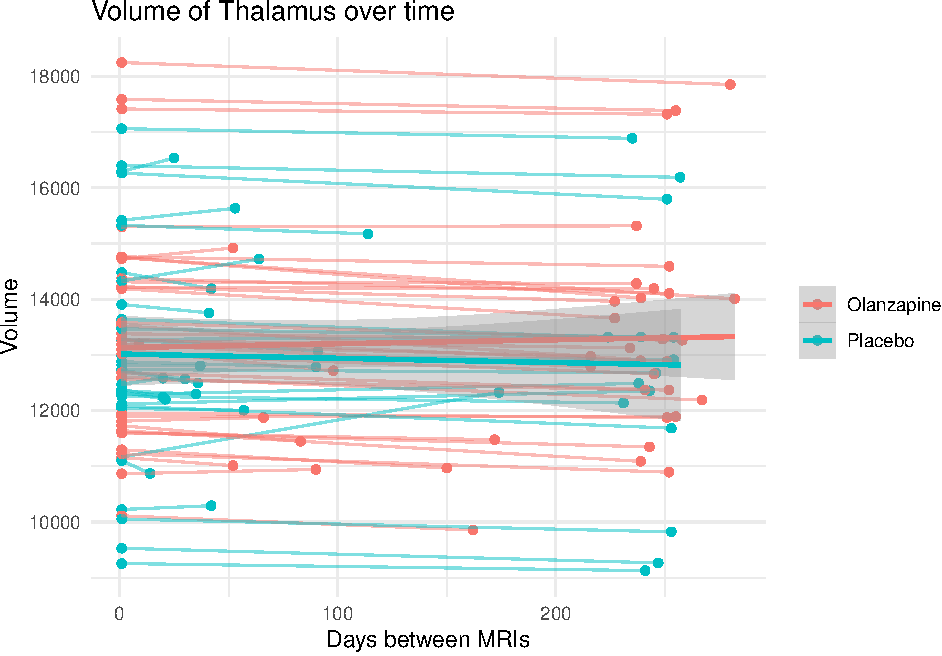
\includegraphics{10_STOPPD_freesurfer_subcortical_files/figure-latex/RCTRelapse_Thalamus_plot-1.pdf}

\begin{Shaded}
\begin{Highlighting}[]
\CommentTok{#run mixed linear model, with covariates}
\NormalTok{  fit_all <-}\StringTok{ }\KeywordTok{lmer}\NormalTok{(volume }\OperatorTok{~}\StringTok{ }\NormalTok{RandomArm}\OperatorTok{*}\NormalTok{model_days }\OperatorTok{+}\StringTok{ }\NormalTok{sex }\OperatorTok{+}\StringTok{ }\NormalTok{age }\OperatorTok{+}\StringTok{ }\NormalTok{(}\DecValTok{1}\OperatorTok{|}\NormalTok{STUDYID), }\DataTypeTok{data=}\NormalTok{ RCTRelapse_Thalamus)}
  \KeywordTok{print}\NormalTok{(fit_all)}
\end{Highlighting}
\end{Shaded}

\begin{verbatim}
## Linear mixed model fit by REML ['lmerModLmerTest']
## Formula: volume ~ RandomArm * model_days + sex + age + (1 | STUDYID)
##    Data: RCTRelapse_Thalamus
## REML criterion at convergence: 2193.44
## Random effects:
##  Groups   Name        Std.Dev.
##  STUDYID  (Intercept) 1396.1  
##  Residual              171.2  
## Number of obs: 144, groups:  STUDYID, 72
## Fixed Effects:
##                 (Intercept)             RandomArmPlacebo  
##                  15637.4008                    -181.4066  
##                  model_days                         sexM  
##                     -1.1851                    1898.4711  
##                         age  RandomArmPlacebo:model_days  
##                    -58.6352                       0.8093
\end{verbatim}

\begin{Shaded}
\begin{Highlighting}[]
  \KeywordTok{summary}\NormalTok{(fit_all)}
\end{Highlighting}
\end{Shaded}

\begin{verbatim}
## Linear mixed model fit by REML. t-tests use Satterthwaite's method [
## lmerModLmerTest]
## Formula: volume ~ RandomArm * model_days + sex + age + (1 | STUDYID)
##    Data: RCTRelapse_Thalamus
## 
## REML criterion at convergence: 2193.4
## 
## Scaled residuals: 
##     Min      1Q  Median      3Q     Max 
## -3.6119 -0.4282  0.0145  0.3924  3.5470 
## 
## Random effects:
##  Groups   Name        Variance Std.Dev.
##  STUDYID  (Intercept) 1949229  1396.1  
##  Residual               29305   171.2  
## Number of obs: 144, groups:  STUDYID, 72
## 
## Fixed effects:
##                               Estimate Std. Error         df t value
## (Intercept)                 15637.4008   645.0482    68.1290  24.242
## RandomArmPlacebo             -181.4066   332.4480    68.7735  -0.546
## model_days                     -1.1851     0.1804    70.1127  -6.570
## sexM                         1898.4711   332.6682    67.9899   5.707
## age                           -58.6352    10.8628    67.9907  -5.398
## RandomArmPlacebo:model_days     0.8093     0.3046    70.2726   2.657
##                             Pr(>|t|)    
## (Intercept)                  < 2e-16 ***
## RandomArmPlacebo             0.58706    
## model_days                  7.46e-09 ***
## sexM                        2.75e-07 ***
## age                         9.26e-07 ***
## RandomArmPlacebo:model_days  0.00976 ** 
## ---
## Signif. codes:  0 '***' 0.001 '**' 0.01 '*' 0.05 '.' 0.1 ' ' 1
## 
## Correlation of Fixed Effects:
##             (Intr) RndmAP mdl_dy sexM   age   
## RndmArmPlcb -0.201                            
## model_days  -0.032  0.056                     
## sexM        -0.172  0.037  0.000              
## age         -0.903 -0.054  0.003 -0.079       
## RndmArmPl:_  0.018 -0.074 -0.592  0.002 -0.001
\end{verbatim}

\begin{Shaded}
\begin{Highlighting}[]
\CommentTok{#run mixed linear model, with covariates}
\NormalTok{  fit_all <-}\StringTok{ }\KeywordTok{lmer}\NormalTok{(volume }\OperatorTok{~}\StringTok{ }\NormalTok{RandomArm}\OperatorTok{*}\NormalTok{model_days }\OperatorTok{+}\StringTok{ }\NormalTok{sex }\OperatorTok{+}\StringTok{ }\NormalTok{age }\OperatorTok{+}\StringTok{ }\NormalTok{site }\OperatorTok{+}\StringTok{ }\NormalTok{(}\DecValTok{1}\OperatorTok{|}\NormalTok{STUDYID), }\DataTypeTok{data=}\NormalTok{ RCTRelapse_Thalamus)}
  \KeywordTok{print}\NormalTok{(fit_all)}
\end{Highlighting}
\end{Shaded}

\begin{verbatim}
## Linear mixed model fit by REML ['lmerModLmerTest']
## Formula: 
## volume ~ RandomArm * model_days + sex + age + site + (1 | STUDYID)
##    Data: RCTRelapse_Thalamus
## REML criterion at convergence: 2140.5
## Random effects:
##  Groups   Name        Std.Dev.
##  STUDYID  (Intercept) 1313.0  
##  Residual              171.2  
## Number of obs: 144, groups:  STUDYID, 72
## Fixed Effects:
##                 (Intercept)             RandomArmPlacebo  
##                  15877.4970                    -149.6319  
##                  model_days                         sexM  
##                     -1.1878                    1844.5154  
##                         age                      siteMAS  
##                    -61.8649                    -822.5404  
##                     siteNKI                      sitePMC  
##                    821.9333                      37.9774  
## RandomArmPlacebo:model_days  
##                      0.8111
\end{verbatim}

\begin{Shaded}
\begin{Highlighting}[]
  \KeywordTok{summary}\NormalTok{(fit_all)}
\end{Highlighting}
\end{Shaded}

\begin{verbatim}
## Linear mixed model fit by REML. t-tests use Satterthwaite's method [
## lmerModLmerTest]
## Formula: 
## volume ~ RandomArm * model_days + sex + age + site + (1 | STUDYID)
##    Data: RCTRelapse_Thalamus
## 
## REML criterion at convergence: 2140.5
## 
## Scaled residuals: 
##     Min      1Q  Median      3Q     Max 
## -3.5816 -0.4404  0.0083  0.3873  3.5784 
## 
## Random effects:
##  Groups   Name        Variance Std.Dev.
##  STUDYID  (Intercept) 1724006  1313.0  
##  Residual               29304   171.2  
## Number of obs: 144, groups:  STUDYID, 72
## 
## Fixed effects:
##                               Estimate Std. Error         df t value
## (Intercept)                 15877.4970   637.1250    65.1359  24.921
## RandomArmPlacebo             -149.6319   317.2828    65.8206  -0.472
## model_days                     -1.1878     0.1804    70.1251  -6.586
## sexM                         1844.5154   317.2625    64.9936   5.814
## age                           -61.8649    10.2955    64.9952  -6.009
## siteMAS                      -822.5404   402.5790    64.9957  -2.043
## siteNKI                       821.9333   446.1341    64.9957   1.842
## sitePMC                        37.9774   459.0477    64.9931   0.083
## RandomArmPlacebo:model_days     0.8111     0.3046    70.3103   2.663
##                             Pr(>|t|)    
## (Intercept)                  < 2e-16 ***
## RandomArmPlacebo              0.6388    
## model_days                  7.00e-09 ***
## sexM                        2.02e-07 ***
## age                         9.35e-08 ***
## siteMAS                       0.0451 *  
## siteNKI                       0.0700 .  
## sitePMC                       0.9343    
## RandomArmPlacebo:model_days   0.0096 ** 
## ---
## Signif. codes:  0 '***' 0.001 '**' 0.01 '*' 0.05 '.' 0.1 ' ' 1
## 
## Correlation of Fixed Effects:
##             (Intr) RndmAP mdl_dy sexM   age    sitMAS sitNKI sitPMC
## RndmArmPlcb -0.140                                                 
## model_days  -0.033  0.059                                          
## sexM        -0.130  0.055  0.001                                   
## age         -0.882 -0.066  0.004 -0.076                            
## siteMAS     -0.292 -0.147  0.004 -0.066  0.108                     
## siteNKI     -0.175 -0.119 -0.004 -0.119  0.010  0.357              
## sitePMC     -0.153 -0.089  0.000 -0.144 -0.009  0.343  0.319       
## RndmArmPl:_  0.018 -0.078 -0.592  0.001 -0.001  0.000  0.004  0.001
\end{verbatim}

\subsubsection{Striatum}\label{striatum-1}

\begin{Shaded}
\begin{Highlighting}[]
\CommentTok{#restructure data for RCT & Relapse participants (N=72)}
\NormalTok{  RCTRelapse_Striatum <-}\StringTok{ }\NormalTok{ana_df }\OperatorTok
\StringTok{    }\KeywordTok{gather}\NormalTok{(oldcolname, volume, Striatum_}\DecValTok{01}\NormalTok{, Striatum_}\DecValTok{02}\NormalTok{) }\OperatorTok
\StringTok{    }\KeywordTok{mutate}\NormalTok{(}\DataTypeTok{model_days =} \KeywordTok{if_else}\NormalTok{(oldcolname }\OperatorTok{==}\StringTok{ "Striatum_01"}\NormalTok{, }\DecValTok{1}\NormalTok{, dateDiff))}

\NormalTok{RCTRelapse_Striatum }\OperatorTok\StringTok{ }\KeywordTok{filter}\NormalTok{(model_days }\OperatorTok{==}\StringTok{ }\DecValTok{1}\NormalTok{) }\OperatorTok\StringTok{ }\KeywordTok{count}\NormalTok{(randomization) }\OperatorTok\StringTok{ }\NormalTok{knitr}\OperatorTok{::}\KeywordTok{kable}\NormalTok{() }
\end{Highlighting}
\end{Shaded}

\begin{tabular}{l|r}
\hline
randomization & n\\
\hline
O & 38\\
\hline
P & 34\\
\hline
\end{tabular}

\begin{Shaded}
\begin{Highlighting}[]
\CommentTok{#plot all data, including outlier (participant 210030)}
\NormalTok{  RCTRelapse_Striatum }\OperatorTok
\StringTok{   }\KeywordTok{ggplot}\NormalTok{(}\KeywordTok{aes}\NormalTok{(}\DataTypeTok{x=}\NormalTok{model_days, }\DataTypeTok{y=}\NormalTok{volume, }\DataTypeTok{colour=}\NormalTok{RandomArm)) }\OperatorTok{+}\StringTok{ }
\StringTok{   }\KeywordTok{geom_point}\NormalTok{() }\OperatorTok{+}\StringTok{ }
\StringTok{   }\KeywordTok{geom_line}\NormalTok{(}\KeywordTok{aes}\NormalTok{(}\DataTypeTok{group=}\NormalTok{STUDYID), }\DataTypeTok{alpha =} \FloatTok{0.5}\NormalTok{) }\OperatorTok{+}\StringTok{ }
\StringTok{   }\KeywordTok{geom_smooth}\NormalTok{(}\DataTypeTok{method=}\StringTok{"lm"}\NormalTok{, }\DataTypeTok{formula=}\NormalTok{y}\OperatorTok{~}\KeywordTok{poly}\NormalTok{(x,}\DecValTok{1}\NormalTok{)) }\OperatorTok{+}
\StringTok{   }\KeywordTok{ggtitle}\NormalTok{(}\StringTok{"Volume of Striatum over time"}\NormalTok{) }\OperatorTok{+}
\StringTok{   }\KeywordTok{labs}\NormalTok{(}\DataTypeTok{x =} \StringTok{"Days between MRIs"}\NormalTok{, }\DataTypeTok{y =} \StringTok{"Volume"}\NormalTok{, }\DataTypeTok{colour =} \OtherTok{NULL}\NormalTok{) }\OperatorTok{+}
\StringTok{   }\KeywordTok{theme_minimal}\NormalTok{()}
\end{Highlighting}
\end{Shaded}

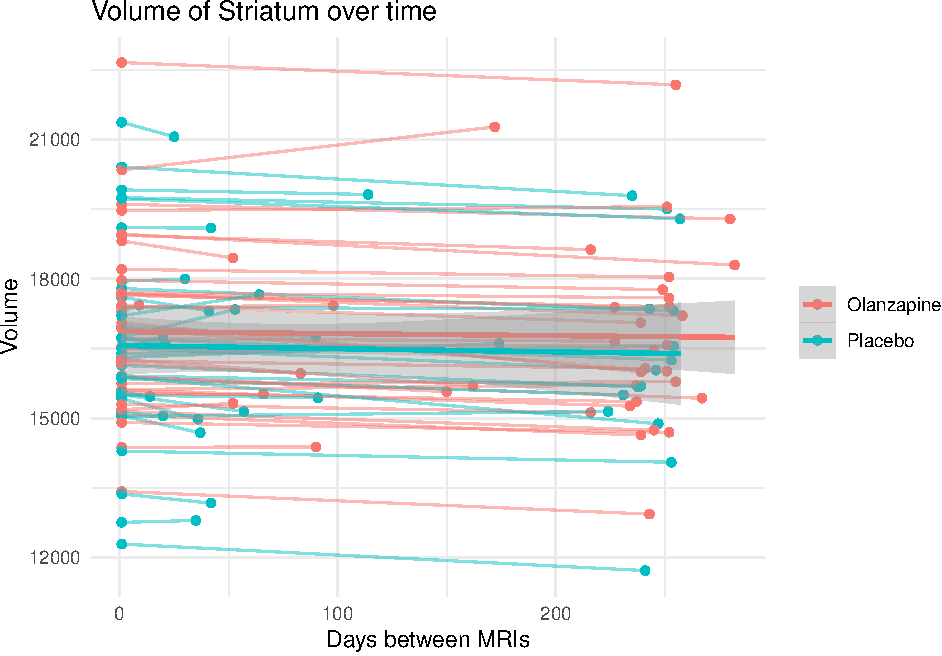
\includegraphics{10_STOPPD_freesurfer_subcortical_files/figure-latex/RCTRelapse_Striatum_plot-1.pdf}

\begin{Shaded}
\begin{Highlighting}[]
\CommentTok{#run mixed linear model, with covariates}
\NormalTok{  fit_all <-}\StringTok{ }\KeywordTok{lmer}\NormalTok{(volume }\OperatorTok{~}\StringTok{ }\NormalTok{RandomArm}\OperatorTok{*}\NormalTok{model_days }\OperatorTok{+}\StringTok{ }\NormalTok{sex }\OperatorTok{+}\StringTok{ }\NormalTok{age }\OperatorTok{+}\StringTok{ }\NormalTok{(}\DecValTok{1}\OperatorTok{|}\NormalTok{STUDYID), }\DataTypeTok{data=}\NormalTok{ RCTRelapse_Striatum)}
  \KeywordTok{print}\NormalTok{(fit_all)}
\end{Highlighting}
\end{Shaded}

\begin{verbatim}
## Linear mixed model fit by REML ['lmerModLmerTest']
## Formula: volume ~ RandomArm * model_days + sex + age + (1 | STUDYID)
##    Data: RCTRelapse_Striatum
## REML criterion at convergence: 2250.495
## Random effects:
##  Groups   Name        Std.Dev.
##  STUDYID  (Intercept) 1674.5  
##  Residual              215.6  
## Number of obs: 144, groups:  STUDYID, 72
## Fixed Effects:
##                 (Intercept)             RandomArmPlacebo  
##                  18786.7886                    -199.5106  
##                  model_days                         sexM  
##                     -1.1427                    1603.1890  
##                         age  RandomArmPlacebo:model_days  
##                    -47.6384                      -0.1886
\end{verbatim}

\begin{Shaded}
\begin{Highlighting}[]
  \KeywordTok{summary}\NormalTok{(fit_all)}
\end{Highlighting}
\end{Shaded}

\begin{verbatim}
## Linear mixed model fit by REML. t-tests use Satterthwaite's method [
## lmerModLmerTest]
## Formula: volume ~ RandomArm * model_days + sex + age + (1 | STUDYID)
##    Data: RCTRelapse_Striatum
## 
## REML criterion at convergence: 2250.5
## 
## Scaled residuals: 
##      Min       1Q   Median       3Q      Max 
## -2.37595 -0.36241  0.03762  0.33458  2.82797 
## 
## Random effects:
##  Groups   Name        Variance Std.Dev.
##  STUDYID  (Intercept) 2804106  1674.5  
##  Residual               46470   215.6  
## Number of obs: 144, groups:  STUDYID, 72
## 
## Fixed effects:
##                               Estimate Std. Error         df t value
## (Intercept)                 18786.7886   774.0095    68.1517  24.272
## RandomArmPlacebo             -199.5106   399.0078    68.8613  -0.500
## model_days                     -1.1427     0.2271    70.1337  -5.031
## sexM                         1603.1890   399.1561    67.9984   4.016
## age                           -47.6384    13.0339    67.9994  -3.655
## RandomArmPlacebo:model_days    -0.1886     0.3836    70.3099  -0.492
##                             Pr(>|t|)    
## (Intercept)                  < 2e-16 ***
## RandomArmPlacebo            0.618657    
## model_days                  3.61e-06 ***
## sexM                        0.000150 ***
## age                         0.000502 ***
## RandomArmPlacebo:model_days 0.624440    
## ---
## Signif. codes:  0 '***' 0.001 '**' 0.01 '*' 0.05 '.' 0.1 ' ' 1
## 
## Correlation of Fixed Effects:
##             (Intr) RndmAP mdl_dy sexM   age   
## RndmArmPlcb -0.202                            
## model_days  -0.034  0.059                     
## sexM        -0.172  0.036  0.000              
## age         -0.903 -0.054  0.003 -0.079       
## RndmArmPl:_  0.019 -0.078 -0.592  0.002 -0.001
\end{verbatim}

\begin{Shaded}
\begin{Highlighting}[]
\CommentTok{#run mixed linear model, with covariates}
\NormalTok{  fit_all <-}\StringTok{ }\KeywordTok{lmer}\NormalTok{(volume }\OperatorTok{~}\StringTok{ }\NormalTok{RandomArm}\OperatorTok{*}\NormalTok{model_days }\OperatorTok{+}\StringTok{ }\NormalTok{sex }\OperatorTok{+}\StringTok{ }\NormalTok{age }\OperatorTok{+}\StringTok{ }\NormalTok{site }\OperatorTok{+}\StringTok{ }\NormalTok{(}\DecValTok{1}\OperatorTok{|}\NormalTok{STUDYID), }\DataTypeTok{data=}\NormalTok{ RCTRelapse_Striatum)}
  \KeywordTok{print}\NormalTok{(fit_all)}
\end{Highlighting}
\end{Shaded}

\begin{verbatim}
## Linear mixed model fit by REML ['lmerModLmerTest']
## Formula: 
## volume ~ RandomArm * model_days + sex + age + site + (1 | STUDYID)
##    Data: RCTRelapse_Striatum
## REML criterion at convergence: 2204.864
## Random effects:
##  Groups   Name        Std.Dev.
##  STUDYID  (Intercept) 1680.8  
##  Residual              215.6  
## Number of obs: 144, groups:  STUDYID, 72
## Fixed Effects:
##                 (Intercept)             RandomArmPlacebo  
##                  19124.4744                    -100.8250  
##                  model_days                         sexM  
##                     -1.1423                    1673.9180  
##                         age                      siteMAS  
##                    -48.9143                    -595.3613  
##                     siteNKI                      sitePMC  
##                   -807.5124                    -307.2624  
## RandomArmPlacebo:model_days  
##                     -0.1903
\end{verbatim}

\begin{Shaded}
\begin{Highlighting}[]
  \KeywordTok{summary}\NormalTok{(fit_all)}
\end{Highlighting}
\end{Shaded}

\begin{verbatim}
## Linear mixed model fit by REML. t-tests use Satterthwaite's method [
## lmerModLmerTest]
## Formula: 
## volume ~ RandomArm * model_days + sex + age + site + (1 | STUDYID)
##    Data: RCTRelapse_Striatum
## 
## REML criterion at convergence: 2204.9
## 
## Scaled residuals: 
##      Min       1Q   Median       3Q      Max 
## -2.38638 -0.35547  0.03791  0.32934  2.81721 
## 
## Random effects:
##  Groups   Name        Variance Std.Dev.
##  STUDYID  (Intercept) 2825222  1680.8  
##  Residual               46470   215.6  
## Number of obs: 144, groups:  STUDYID, 72
## 
## Fixed effects:
##                               Estimate Std. Error         df t value
## (Intercept)                 19124.4744   815.4829    65.1363  23.452
## RandomArmPlacebo             -100.8250   406.0694    65.7992  -0.248
## model_days                     -1.1423     0.2271    70.1259  -5.029
## sexM                         1673.9180   406.0846    64.9986   4.122
## age                           -48.9143    13.1779    65.0002  -3.712
## siteMAS                      -595.3613   515.2865    65.0006  -1.155
## siteNKI                      -807.5124   571.0354    65.0006  -1.414
## sitePMC                      -307.2624   587.5646    64.9981  -0.523
## RandomArmPlacebo:model_days    -0.1903     0.3836    70.3052  -0.496
##                             Pr(>|t|)    
## (Intercept)                  < 2e-16 ***
## RandomArmPlacebo            0.804680    
## model_days                  3.63e-06 ***
## sexM                        0.000109 ***
## age                         0.000429 ***
## siteMAS                     0.252157    
## siteNKI                     0.162099    
## sitePMC                     0.602793    
## RandomArmPlacebo:model_days 0.621329    
## ---
## Signif. codes:  0 '***' 0.001 '**' 0.01 '*' 0.05 '.' 0.1 ' ' 1
## 
## Correlation of Fixed Effects:
##             (Intr) RndmAP mdl_dy sexM   age    sitMAS sitNKI sitPMC
## RndmArmPlcb -0.140                                                 
## model_days  -0.033  0.058                                          
## sexM        -0.130  0.055  0.001                                   
## age         -0.882 -0.066  0.004 -0.076                            
## siteMAS     -0.292 -0.147  0.004 -0.066  0.108                     
## siteNKI     -0.175 -0.119 -0.004 -0.119  0.010  0.357              
## sitePMC     -0.153 -0.089  0.000 -0.144 -0.009  0.343  0.319       
## RndmArmPl:_  0.017 -0.077 -0.592  0.001 -0.001  0.000  0.004  0.001
\end{verbatim}

\subsubsection{Hippocampus}\label{hippocampus-1}

\begin{Shaded}
\begin{Highlighting}[]
\CommentTok{#restructure data for RCT & Relapse participants (N=72)}
\NormalTok{  RCTRelapse_Hippocampus <-}\StringTok{ }\NormalTok{ana_df }\OperatorTok
\StringTok{    }\KeywordTok{gather}\NormalTok{(oldcolname, volume, Hippocampus_}\DecValTok{01}\NormalTok{, Hippocampus_}\DecValTok{02}\NormalTok{) }\OperatorTok
\StringTok{    }\KeywordTok{mutate}\NormalTok{(}\DataTypeTok{model_days =} \KeywordTok{if_else}\NormalTok{(oldcolname }\OperatorTok{==}\StringTok{ "Hippocampus_01"}\NormalTok{, }\DecValTok{1}\NormalTok{, dateDiff))}

\NormalTok{RCTRelapse_Hippocampus }\OperatorTok\StringTok{ }\KeywordTok{filter}\NormalTok{(model_days }\OperatorTok{==}\StringTok{ }\DecValTok{1}\NormalTok{) }\OperatorTok\StringTok{ }\KeywordTok{count}\NormalTok{(randomization) }\OperatorTok\StringTok{ }\NormalTok{knitr}\OperatorTok{::}\KeywordTok{kable}\NormalTok{() }
\end{Highlighting}
\end{Shaded}

\begin{tabular}{l|r}
\hline
randomization & n\\
\hline
O & 38\\
\hline
P & 34\\
\hline
\end{tabular}

\begin{Shaded}
\begin{Highlighting}[]
\CommentTok{#plot all data, including outlier (participant 210030)}
\NormalTok{  RCTRelapse_Hippocampus }\OperatorTok
\StringTok{   }\KeywordTok{ggplot}\NormalTok{(}\KeywordTok{aes}\NormalTok{(}\DataTypeTok{x=}\NormalTok{model_days, }\DataTypeTok{y=}\NormalTok{volume, }\DataTypeTok{colour=}\NormalTok{RandomArm)) }\OperatorTok{+}\StringTok{ }
\StringTok{   }\KeywordTok{geom_point}\NormalTok{() }\OperatorTok{+}\StringTok{ }
\StringTok{   }\KeywordTok{geom_line}\NormalTok{(}\KeywordTok{aes}\NormalTok{(}\DataTypeTok{group=}\NormalTok{STUDYID), }\DataTypeTok{alpha =} \FloatTok{0.5}\NormalTok{) }\OperatorTok{+}\StringTok{ }
\StringTok{   }\KeywordTok{geom_smooth}\NormalTok{(}\DataTypeTok{method=}\StringTok{"lm"}\NormalTok{, }\DataTypeTok{formula=}\NormalTok{y}\OperatorTok{~}\KeywordTok{poly}\NormalTok{(x,}\DecValTok{1}\NormalTok{)) }\OperatorTok{+}
\StringTok{   }\KeywordTok{ggtitle}\NormalTok{(}\StringTok{"Volume of Hippocampus over time"}\NormalTok{) }\OperatorTok{+}
\StringTok{   }\KeywordTok{labs}\NormalTok{(}\DataTypeTok{x =} \StringTok{"Days between MRIs"}\NormalTok{, }\DataTypeTok{y =} \StringTok{"Volume"}\NormalTok{, }\DataTypeTok{colour =} \OtherTok{NULL}\NormalTok{) }\OperatorTok{+}
\StringTok{   }\KeywordTok{theme_minimal}\NormalTok{()}
\end{Highlighting}
\end{Shaded}

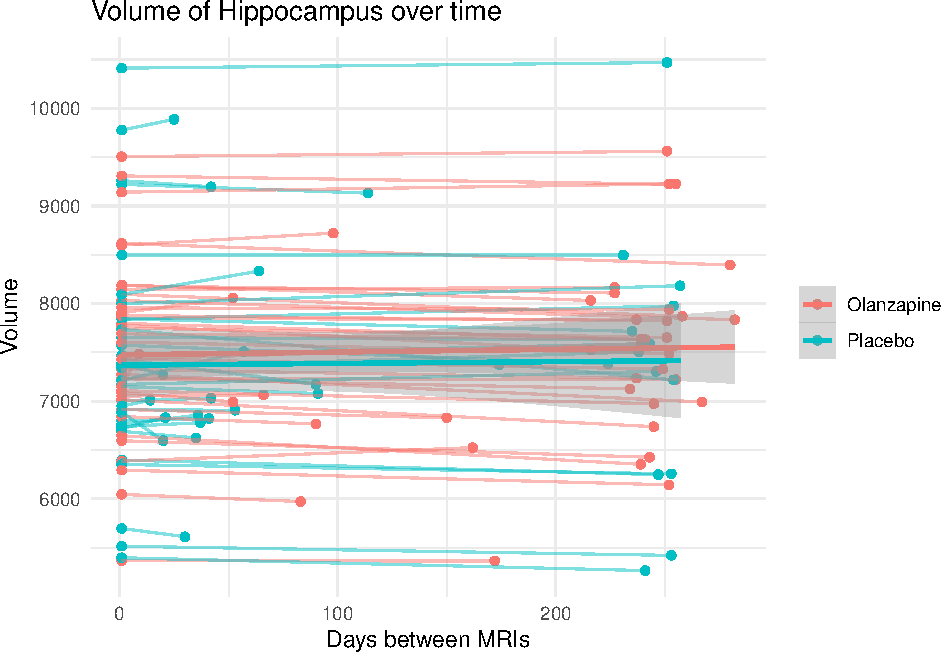
\includegraphics{10_STOPPD_freesurfer_subcortical_files/figure-latex/RCTRelapse_Hippocampus_plot-1.pdf}

\begin{Shaded}
\begin{Highlighting}[]
\CommentTok{#run mixed linear model, with covariates}
\NormalTok{  fit_all <-}\StringTok{ }\KeywordTok{lmer}\NormalTok{(volume }\OperatorTok{~}\StringTok{ }\NormalTok{RandomArm}\OperatorTok{*}\NormalTok{model_days }\OperatorTok{+}\StringTok{ }\NormalTok{sex }\OperatorTok{+}\StringTok{ }\NormalTok{age }\OperatorTok{+}\StringTok{ }\NormalTok{(}\DecValTok{1}\OperatorTok{|}\NormalTok{STUDYID), }\DataTypeTok{data=}\NormalTok{ RCTRelapse_Hippocampus)}
  \KeywordTok{print}\NormalTok{(fit_all)}
\end{Highlighting}
\end{Shaded}

\begin{verbatim}
## Linear mixed model fit by REML ['lmerModLmerTest']
## Formula: volume ~ RandomArm * model_days + sex + age + (1 | STUDYID)
##    Data: RCTRelapse_Hippocampus
## REML criterion at convergence: 2049.905
## Random effects:
##  Groups   Name        Std.Dev.
##  STUDYID  (Intercept) 840.5   
##  Residual             100.6   
## Number of obs: 144, groups:  STUDYID, 72
## Fixed Effects:
##                 (Intercept)             RandomArmPlacebo  
##                   8989.3972                     -84.5737  
##                  model_days                         sexM  
##                     -0.4047                     607.4115  
##                         age  RandomArmPlacebo:model_days  
##                    -31.6143                       0.2634
\end{verbatim}

\begin{Shaded}
\begin{Highlighting}[]
  \KeywordTok{summary}\NormalTok{(fit_all)}
\end{Highlighting}
\end{Shaded}

\begin{verbatim}
## Linear mixed model fit by REML. t-tests use Satterthwaite's method [
## lmerModLmerTest]
## Formula: volume ~ RandomArm * model_days + sex + age + (1 | STUDYID)
##    Data: RCTRelapse_Hippocampus
## 
## REML criterion at convergence: 2049.9
## 
## Scaled residuals: 
##      Min       1Q   Median       3Q      Max 
## -2.41294 -0.41410 -0.00566  0.40252  2.36012 
## 
## Random effects:
##  Groups   Name        Variance Std.Dev.
##  STUDYID  (Intercept) 706389   840.5   
##  Residual              10111   100.6   
## Number of obs: 144, groups:  STUDYID, 72
## 
## Fixed effects:
##                              Estimate Std. Error        df t value
## (Intercept)                 8989.3972   388.2347   68.1293  23.155
## RandomArmPlacebo             -84.5737   200.0678   68.7432  -0.423
## model_days                    -0.4047     0.1060   70.1138  -3.820
## sexM                         607.4115   200.2276   67.9968   3.034
## age                          -31.6143     6.5381   67.9975  -4.835
## RandomArmPlacebo:model_days    0.2634     0.1790   70.2661   1.472
##                             Pr(>|t|)    
## (Intercept)                  < 2e-16 ***
## RandomArmPlacebo            0.673815    
## model_days                  0.000285 ***
## sexM                        0.003420 ** 
## age                         7.94e-06 ***
## RandomArmPlacebo:model_days 0.145501    
## ---
## Signif. codes:  0 '***' 0.001 '**' 0.01 '*' 0.05 '.' 0.1 ' ' 1
## 
## Correlation of Fixed Effects:
##             (Intr) RndmAP mdl_dy sexM   age   
## RndmArmPlcb -0.201                            
## model_days  -0.031  0.055                     
## sexM        -0.172  0.037  0.000              
## age         -0.903 -0.054  0.003 -0.079       
## RndmArmPl:_  0.017 -0.073 -0.592  0.002 -0.001
\end{verbatim}

\begin{Shaded}
\begin{Highlighting}[]
\CommentTok{#run mixed linear model, with covariates}
\NormalTok{  fit_all <-}\StringTok{ }\KeywordTok{lmer}\NormalTok{(volume }\OperatorTok{~}\StringTok{ }\NormalTok{RandomArm}\OperatorTok{*}\NormalTok{model_days }\OperatorTok{+}\StringTok{ }\NormalTok{sex }\OperatorTok{+}\StringTok{ }\NormalTok{age }\OperatorTok{+}\StringTok{ }\NormalTok{site }\OperatorTok{+}\StringTok{ }\NormalTok{(}\DecValTok{1}\OperatorTok{|}\NormalTok{STUDYID), }\DataTypeTok{data=}\NormalTok{ RCTRelapse_Hippocampus)}
  \KeywordTok{print}\NormalTok{(fit_all)}
\end{Highlighting}
\end{Shaded}

\begin{verbatim}
## Linear mixed model fit by REML ['lmerModLmerTest']
## Formula: 
## volume ~ RandomArm * model_days + sex + age + site + (1 | STUDYID)
##    Data: RCTRelapse_Hippocampus
## REML criterion at convergence: 2005.898
## Random effects:
##  Groups   Name        Std.Dev.
##  STUDYID  (Intercept) 827.3   
##  Residual             100.6   
## Number of obs: 144, groups:  STUDYID, 72
## Fixed Effects:
##                 (Intercept)             RandomArmPlacebo  
##                   8920.7798                    -106.7365  
##                  model_days                         sexM  
##                     -0.4048                     548.9133  
##                         age                      siteMAS  
##                    -32.1879                      46.0261  
##                     siteNKI                      sitePMC  
##                    116.0375                     631.6705  
## RandomArmPlacebo:model_days  
##                      0.2637
\end{verbatim}

\begin{Shaded}
\begin{Highlighting}[]
  \KeywordTok{summary}\NormalTok{(fit_all)}
\end{Highlighting}
\end{Shaded}

\begin{verbatim}
## Linear mixed model fit by REML. t-tests use Satterthwaite's method [
## lmerModLmerTest]
## Formula: 
## volume ~ RandomArm * model_days + sex + age + site + (1 | STUDYID)
##    Data: RCTRelapse_Hippocampus
## 
## REML criterion at convergence: 2005.9
## 
## Scaled residuals: 
##      Min       1Q   Median       3Q      Max 
## -2.40104 -0.40874 -0.00025  0.39616  2.37266 
## 
## Random effects:
##  Groups   Name        Variance Std.Dev.
##  STUDYID  (Intercept) 684488   827.3   
##  Residual              10111   100.6   
## Number of obs: 144, groups:  STUDYID, 72
## 
## Fixed effects:
##                              Estimate Std. Error        df t value
## (Intercept)                 8920.7798   401.2060   65.1204  22.235
## RandomArmPlacebo            -106.7365   199.7292   65.7164  -0.534
## model_days                    -0.4048     0.1060   70.1110  -3.820
## sexM                         548.9133   199.7986   64.9966   2.747
## age                          -32.1879     6.4837   64.9980  -4.964
## siteMAS                       46.0261   253.5270   64.9984   0.182
## siteNKI                      116.0375   280.9562   64.9984   0.413
## sitePMC                      631.6705   289.0890   64.9961   2.185
## RandomArmPlacebo:model_days    0.2637     0.1790   70.2722   1.474
##                             Pr(>|t|)    
## (Intercept)                  < 2e-16 ***
## RandomArmPlacebo            0.594864    
## model_days                  0.000285 ***
## sexM                        0.007766 ** 
## age                         5.26e-06 ***
## siteMAS                     0.856506    
## siteNKI                     0.680959    
## sitePMC                     0.032497 *  
## RandomArmPlacebo:model_days 0.145021    
## ---
## Signif. codes:  0 '***' 0.001 '**' 0.01 '*' 0.05 '.' 0.1 ' ' 1
## 
## Correlation of Fixed Effects:
##             (Intr) RndmAP mdl_dy sexM   age    sitMAS sitNKI sitPMC
## RndmArmPlcb -0.140                                                 
## model_days  -0.031  0.055                                          
## sexM        -0.130  0.055  0.001                                   
## age         -0.882 -0.066  0.004 -0.076                            
## siteMAS     -0.292 -0.147  0.004 -0.066  0.108                     
## siteNKI     -0.175 -0.119 -0.004 -0.119  0.010  0.357              
## sitePMC     -0.153 -0.089  0.000 -0.144 -0.009  0.343  0.319       
## RndmArmPl:_  0.017 -0.073 -0.592  0.001 -0.001  0.000  0.004  0.001
\end{verbatim}


\end{document}
